% This file demonstrates how to use the IEEEConf LaTeX2e macro package,
% to prepare a manuscript for proceedings on CD of the conference
% FedCSIS
%
\documentclass[conference]{IEEEtran}
%\documentclass[a4paper]{IEEEconf}

\usepackage{balance}
\IEEEoverridecommandlockouts 
\usepackage[dvips]{graphicx}
\usepackage{algorithmic}
\usepackage{algorithm}
\usepackage{listings}
\usepackage[OT4,T1]{fontenc}
\usepackage[cmex10]{amsmath}
\interdisplaylinepenalty=2500
\usepackage{url}
\usepackage{multirow}
\usepackage{caption}
\usepackage{diagbox}

\newtheorem{remark}{Remark}[section]
\newtheorem{example}[remark]{Example}

\title{Local Search, Brute-Force and Recursion for Selection Operator\thanks{This work was not supported by Velbazhd Software LLC and Bulgarian Ministry of Education and Science.}}

\author{\IEEEauthorblockN{Petar Tomov, Iliyan Zankinski, Todor Balabanov \textsuperscript{\tiny{0000-0003-3139-069X}}}
\IEEEauthorblockA{Institute of Information and Communication Technologies \\ Bulgarian Academy of Sciences \\ acad. Georgi Bonchev Str., block 2, 1113 Sofia, Bulgaria \\p.tomov@iit.bas.bg iliyan@hsi.iccs.bas.bg todorb@iinf.bas.bg}}
%
% Bulgarian Academy of Sciences
% Institute of Information and Communication Technologies
% acad. Georgi Bonchev Str., block 2, office 514, 1113 Sofia, Bulgaria
% http://www.iict.bas.bg/
% iict@bas.bg
%

\begin{document}

\maketitle

\begin{abstract}
Genetic algorithms are heuristics inspired by the processes in the biological evolution. They have a main application in the field of global optimization. The optimization process is organized into three common operations - crossover, mutation, and selection. The crossover and the mutation are used for recombination and do produce new individuals to the population. Selection is used for appointing better parents during the reproduction process \cite{matsui-01}. Many different selection operators are well described in the literature. In the group of the most used are: Proportional Selection, Tournament Selection, Rank-Based Selection, Boltzmann Selection, Soft Brood Selection, Disruptive Selection, Nonlinear Ranking Selection, and Competitive Selection. This study proposes an improvement to recursive brute-force selection by the addition of local search on the level of the brute-force. In every level of recursive descent, all local individuals are recombined with each other (brute-force) as many times as there is an improvement (local search). Only the best-found individual after that is sent to the population of the higher level.
\end{abstract}

\section{Introduction}

\IEEEPARstart{I}{n} the field of meta-heuristic global optimization, genetic algorithms are well known and widely applied. Genetic algorithms have stochastic nature because random or pseudo-random numbers are extensively used in common operators like crossover, mutation, and selection. Finding global optimum is rarely possible and in most cases, genetic algorithms give sub-optimal solutions. Because of the stochastic nature found solutions can differ between different runs of the optimization process. At the same time, the possibilities for different runs are great option for parallel or distributed computing. Mechanisms in natural evolution have inspired the ideas involved in genetic algorithms. Meta-heuristics are most useful for optimization problems in multidimensional spaces with a high degree of non-linearity. A point in multidimensional space (for genetic algorithms it is the solutions space) is presented as vector of values. The set of vectors in the solutions space forms a population of individuals in terms of genetic algorithms. The size of the population is very problem dependent and it is estimated empirically by trial and error approach \cite{alander-01}. The target function is applied to each individual of the population. The result of this calculation gives the individual's fitness value. The fitness value gets better with approaching the optimum. Individuals with better fitness have better chances to mate and to form a new generation. The mating process consists of two common operators - crossover and mutation. Crossover contributes to the exploration of the solutions space when mutation contributes to the exploitation of the solutions space. Genetic algorithms are heavily researched in the last few decades, but there are still directions for improvements. Such direction is the selection operator. This research focuses on searching for optimum to set of benchmark functions by the addition of local search \cite{fellows-01} in brute-force procedure when it is applied in recursive descent \cite{gelfand-01}. 

Selecting parents for mating can be done according many different strategies. The most important target of successful mating is to select as better individuals as possible more often with the hope that they will produce even better offspring. Selecting parents at random will lead to a very slow convergence of the optimization process \cite{wang-01}. The proportional selection \cite{back-01} is one of the first improvements in the selection process. The idea behind it is that each individual receives a crossover chance proportional to its fitness value. Tournament selection \cite{miller-01} is another selection strategy in which by competition between a subset of individuals only winners are nominated for mating. Rank selection \cite{grefenstette-01} on the other side uses ranking of individuals in order to determine their chances for mating. Boltzmann selection \cite{goldberg-01} uses simulated annealing. In this strategy, winners are nominated after a predetermined number of Boltzmann experiments. 

There are many hybrid implementations of the above listed selection strategies. This research proposes a local search extension of the brute-force element in the recursive selection proposed by Tomov, Zankinski, and Balabanov \cite{tomov-01}. A hierarchy of sub-generations is generated and the best-fitted individuals are selected with recursive descent. On each level of recursion single brute-force searching is applied and only one individual is promoted to a higher level. The newly proposed modification applies brute-force search as many times as there is an improvement of the findings, which in fact is a local search extension. 

The rest of the paper is organized as follows: After the introductory part proposition for local search extension to recursive brute-force selection operator is presented; Some experiments and results are presented after that; Paper concludes with a summary of the research and with some directions for a further work.

\section{Local Search Proposition}

The selection operator described in \cite{tomov-01} consists of recursive descent and brute-force. There is a predefined depth of recursion levels. On each level of recursion, there is a genetic algorithm sub-population. The size of sub-populations is equal and it is also predefined. All individuals in the leaves of the recursive tree are randomly generated. The brute-force part of the algorithm consists of the fact that each individual mates with each other in the sub-population. Only the best-found individual is promoted to go in the higher sub-population. Each higher sub-population is fulfilled with individuals promoted from the lower levels. The proposed improvement in this selection procedure states that brute-force should be returned as many times as there is an improvement of the best-found individual (Algorithm \ref{algo01}). 

\begin{algorithm}[tbp]
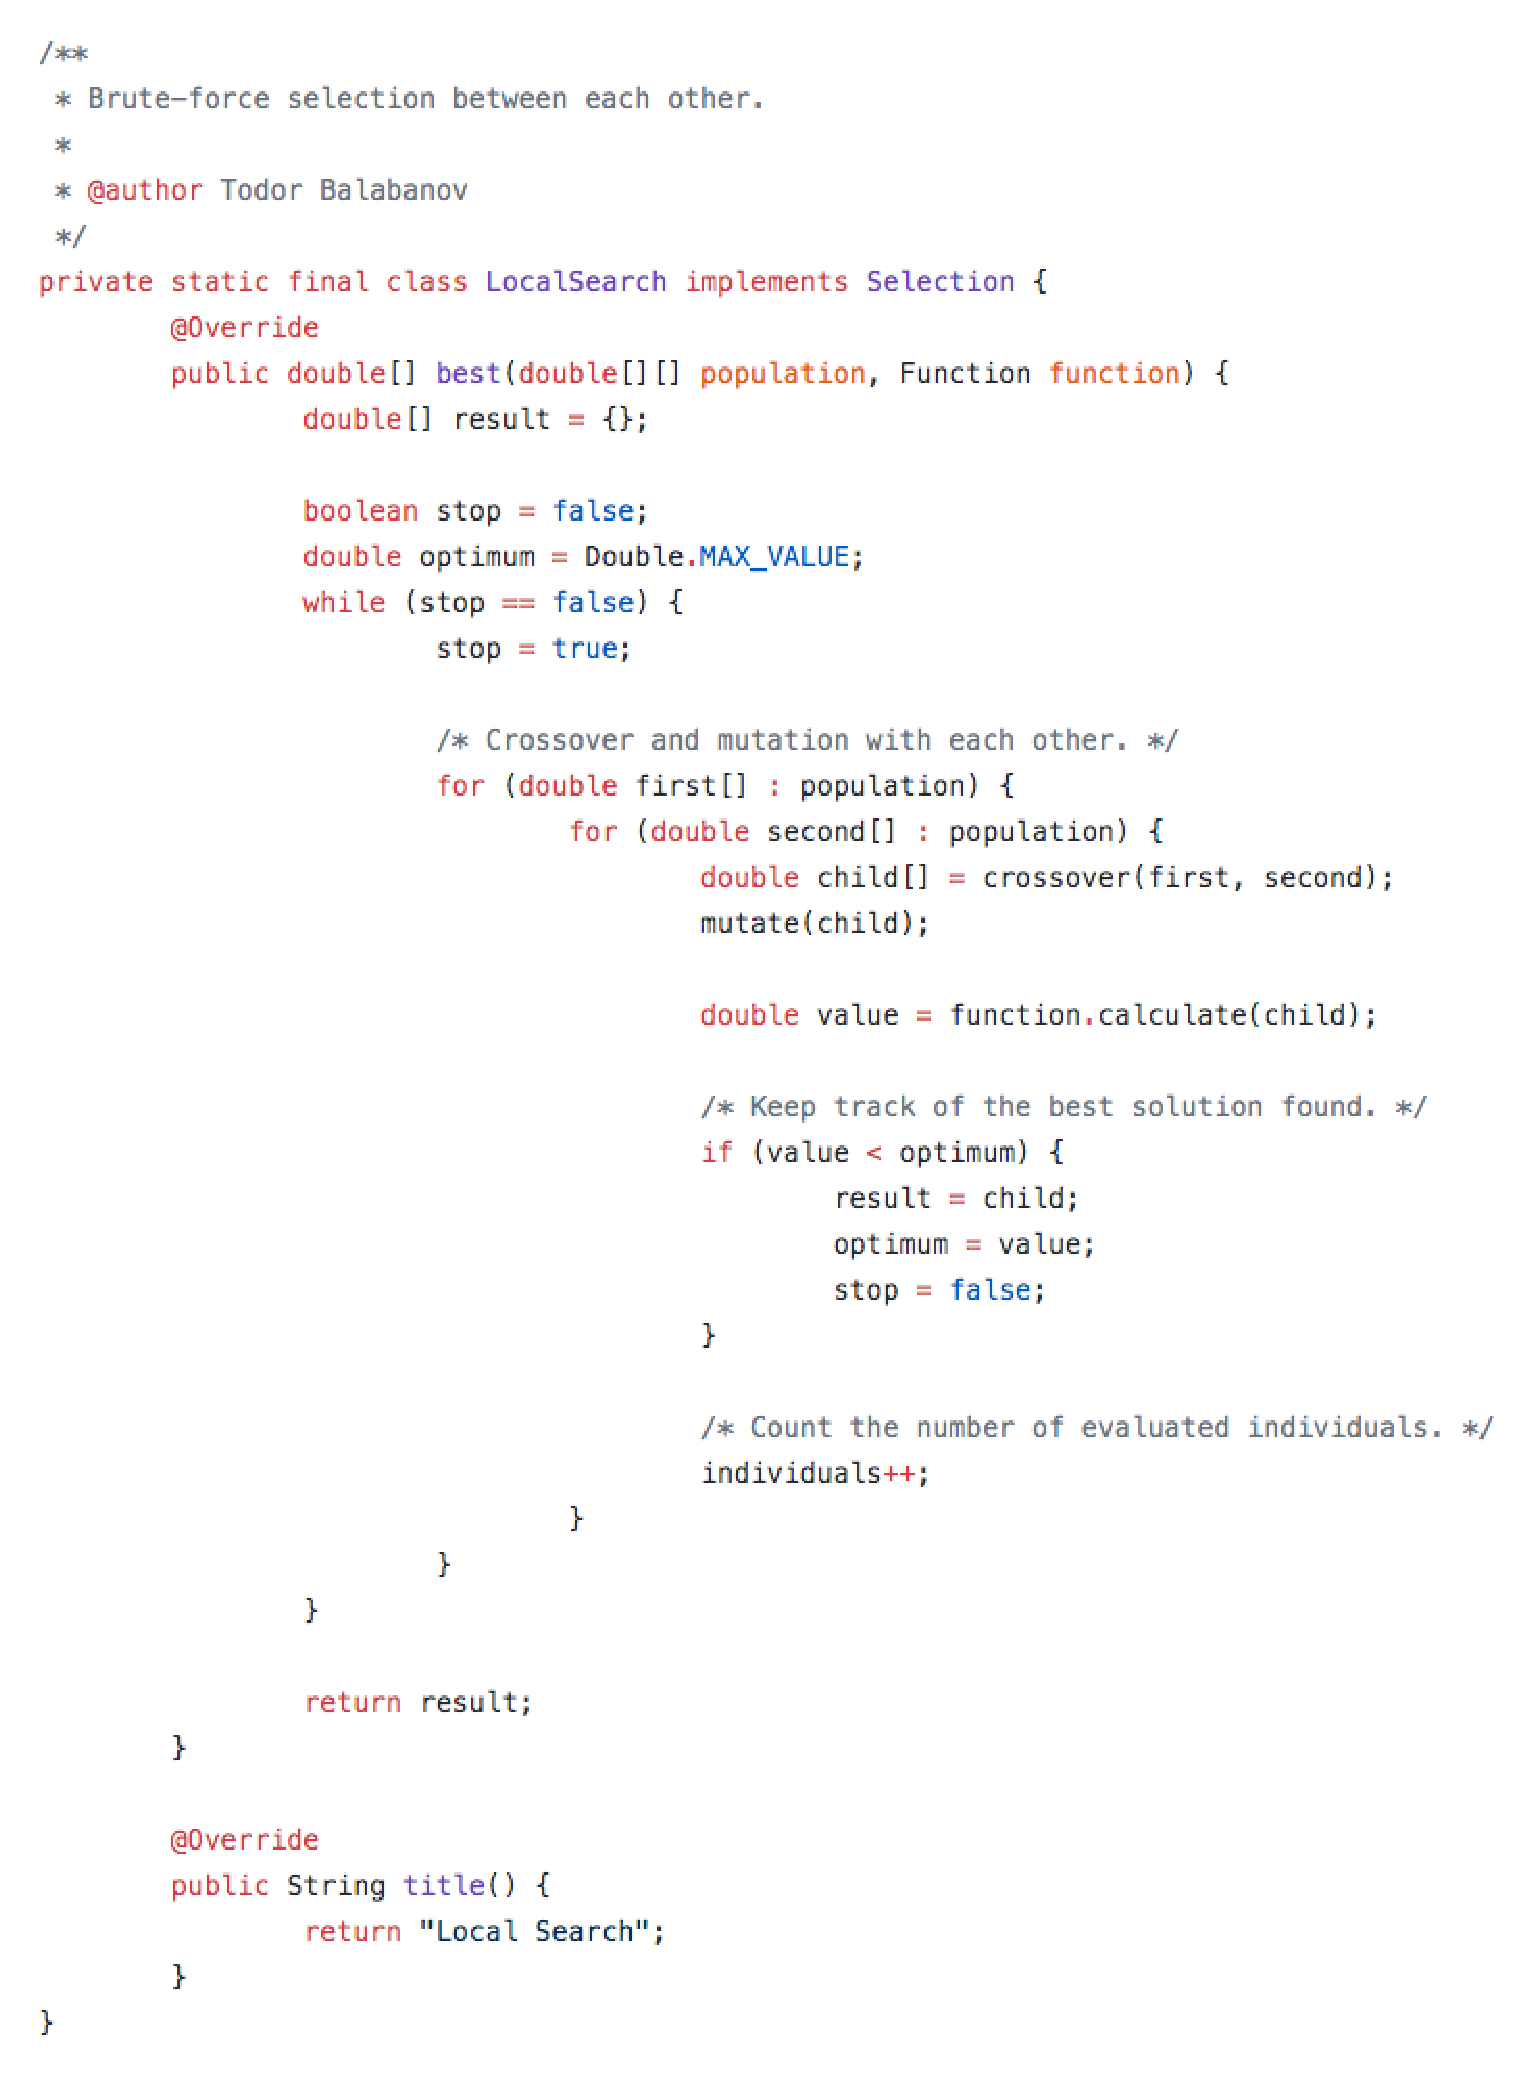
\includegraphics[width=1.0\hsize]{fig01.eps}
\caption{Local search extension.}
\label{algo01}
\end{algorithm}

From one side, such modification dose local search into the surrounding area of the solutions space. On the other side, such modification makes the algorithm with non-deterministic number of individual recombinations. 

\section{Experiments and Results}

All experiments are done in 10000-dimensional solutions space. As benchmark functions are selected five very well known functions: Michalewicz, Ackley, Schwefel, Rastrigin, and Griewank. Algorithms are tested with levels of recursive descent from 2 to 7 and with population size from 2 to 11. Table \ref{tab01} shows the calculation time used in both algorithms for the configuration of recursive descent 7 and population size 11. Table \ref{tab02} shows the total number of individuals evaluation (fitness value calculation) in both algorithms for the configuration of recursive descent 7 and population size 11. The exact numbers achieved in the experiments can be found at this URL address: https://github.com/TodorBalabanov/FedCSIS-Conference-on-Computer-Science-and-Information-Systems-2020/tree/master/Local-Search-Brute-Force-and-Recursion-for-Selection-Operator

\begin{table*}[tbp]
\caption{Calculation time [ms] for recursion level of 7 and population size of 11.}
\centering
\begin{tabular}{|@{\vrule width0ptheight9pt\enspace}l|c|c|c|c|c|c|}
\hline
\hfil\bf \backslashbox{Algorithm}{Funcition}  & \bf Michalewicz & \bf Ackley & \bf Schwefel & \bf Rastrigin & \bf Griewank \\
\hline
\bf Local Search & 1062492546 & 531027435 & 533232986 & 507650704 & 592370933 \\
\hline
\bf Brute-Force & 403141211 & 166733879 & 175069174 & 159862955 & 218428047 \\
\hline
\end{tabular}
\label{tab01}
\end{table*}

\begin{table*}[tbp]
\caption{Number of fitness calculations for recursion level of 7 and population size of 11.}
\centering
\begin{tabular}{|@{\vrule width0ptheight9pt\enspace}l|c|c|c|c|c|c|}
\hline
\hfil\bf \backslashbox{Algorithm}{Funcition}  & \bf Michalewicz & \bf Ackley & \bf Schwefel & \bf Rastrigin & \bf Griewank \\
\hline
\bf Local Search & 641125639 & 641024362 & 640914978 & 641092606 & 640830762 \\
\hline
\bf Brute-Force & 235794757 & 235794757 & 235794757 & 235794757 & 235794757 \\
\hline
\end{tabular}
\label{tab02}
\end{table*}

\begin{table*}[tbp]
\caption{Suboptimal values found for recursion level of 7 and population size of 11.}
\centering
\begin{tabular}{|@{\vrule width0ptheight9pt\enspace}l|c|c|c|c|c|c|}
\hline
\hfil\bf \backslashbox{Algorithm}{Funcition}  & \bf Michalewicz & \bf Ackley & \bf Schwefel & \bf Rastrigin & \bf Griewank \\
\hline
\bf Local Search & -1484.7137949531716 & 21.09334816052046 & 3877924.0971615044 & 170204.87849875208 & 259918.15469527297 \\
\hline
\bf Brute-Force & -1439.2296970724608 & 21.114702255301292 & 3919318.729777085 & 171780.33307271387 & 262621.61053178157 \\
\hline
\end{tabular}
\label{tab03}
\end{table*}

Suboptimal values achieved by both algorithms are presented in Fig. \ref{fig01}-\ref{fig10}. The presented information includes all experimental combinations of recursive descent levels and population sizes. Fig. \ref{fig11}-\ref{fig20} show computational time used. Fig. \ref{fig21}-\ref{fig30} show number of evaluations done during optimization process. Table \ref{tab03} shows suboptimal values found by both algorithms for the configuration of recursive descent 7 and population size 11. Values achieved with the local search extension are closer to the global optimums.

\begin{figure}[tbp]
\centering
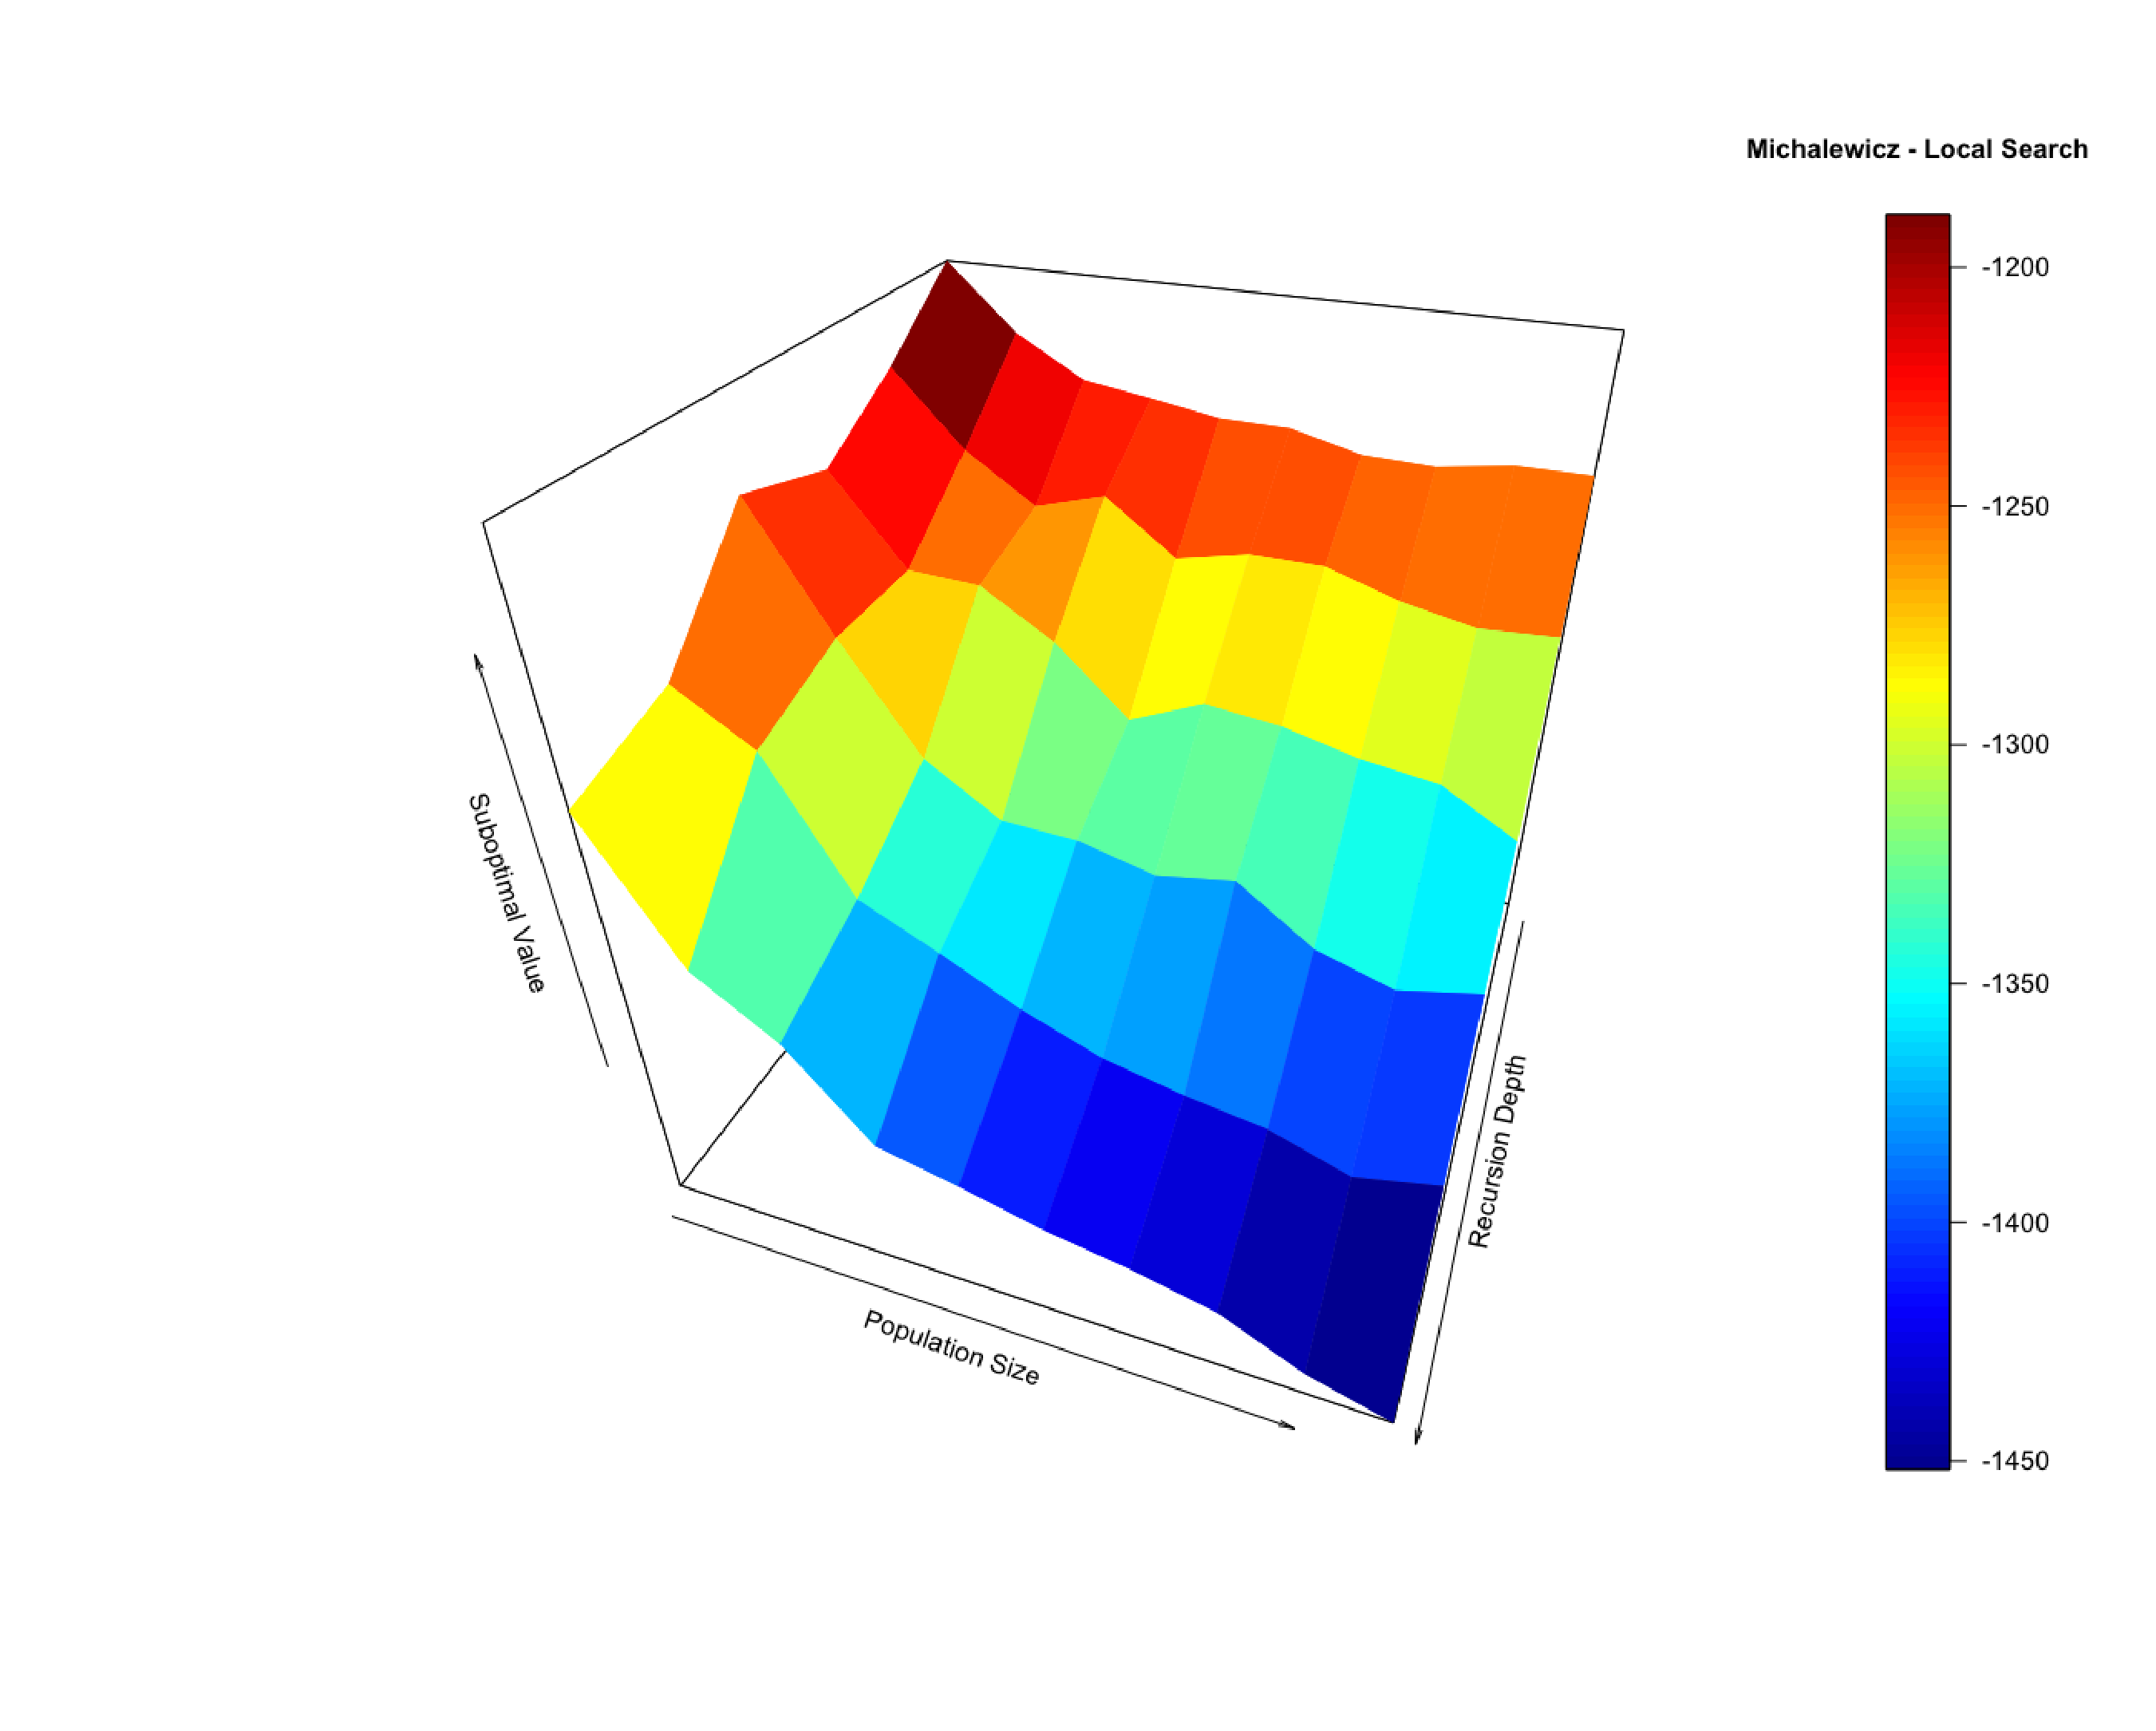
\includegraphics[width=1.0\hsize,height=0.65\hsize]{fig03.eps}
\caption{Michalewicz - Local Search - Suboptimal Values}
\label{fig01}
\end{figure}

\begin{figure}[tbp]
\centering
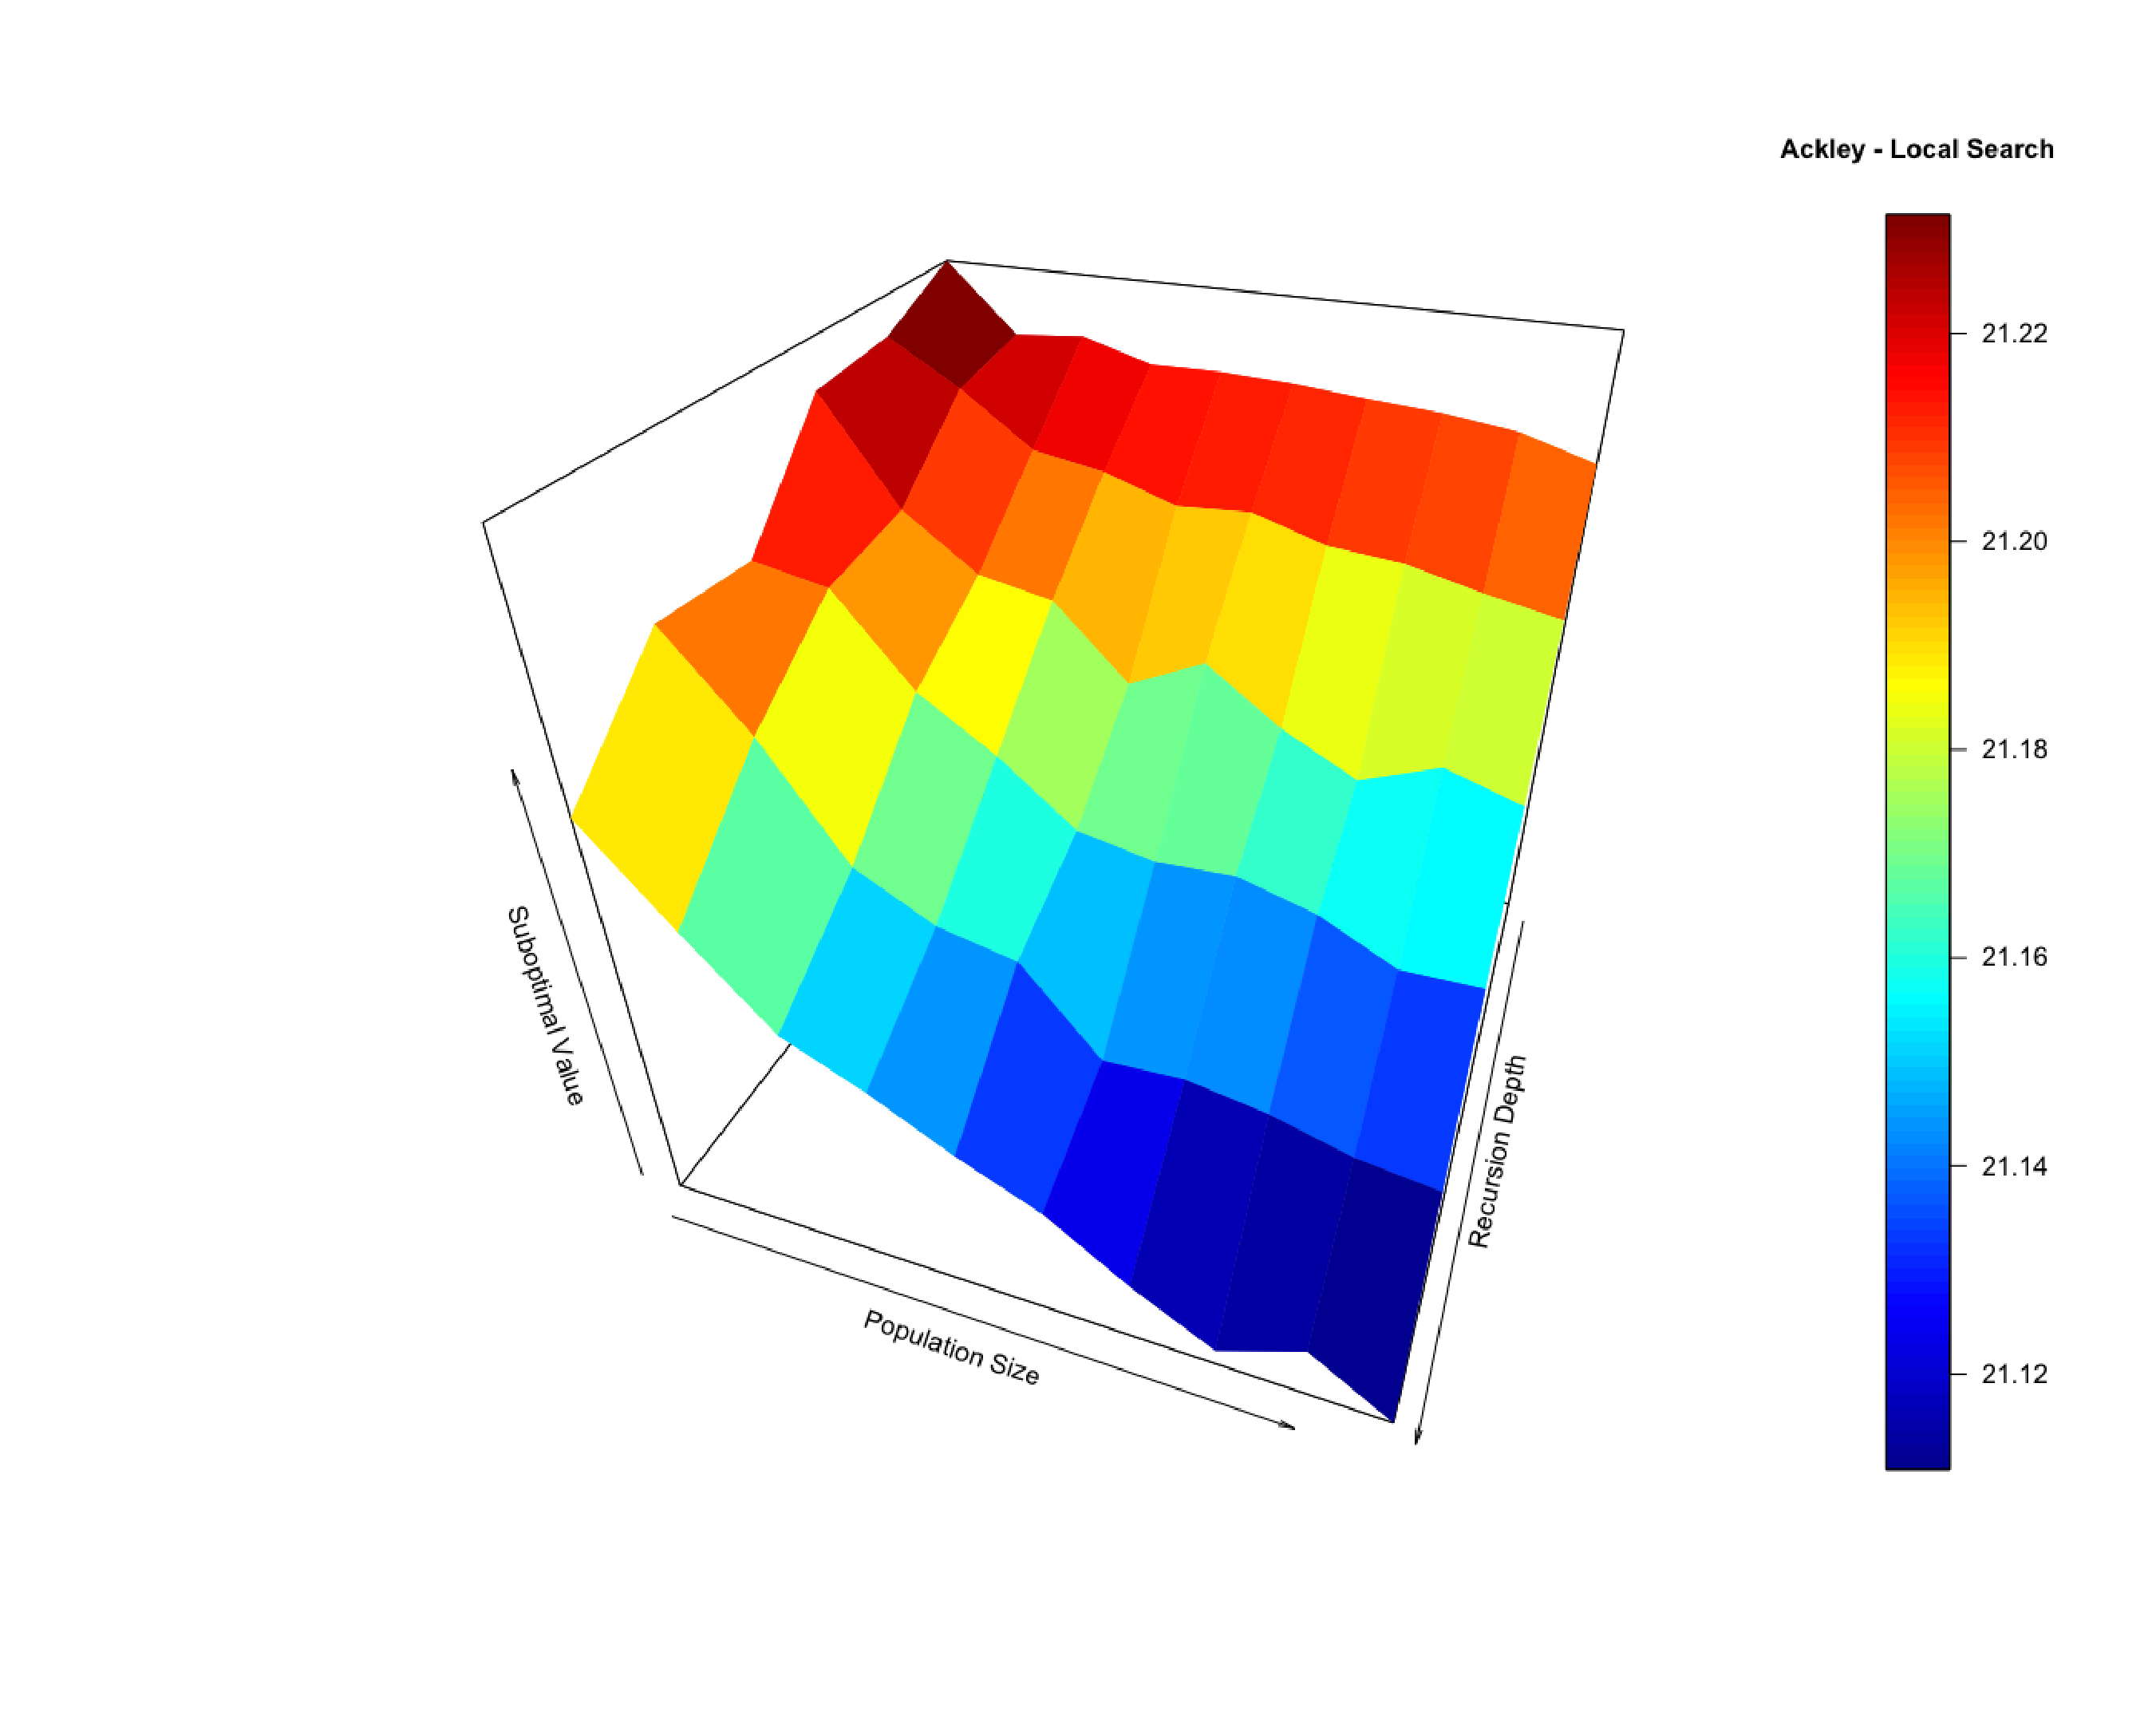
\includegraphics[width=1.0\hsize,height=0.65\hsize]{fig06.eps}
\caption{Ackley - Local Search - Suboptimal Values}
\label{fig02}
\end{figure}

\begin{figure}[tbp]
\centering
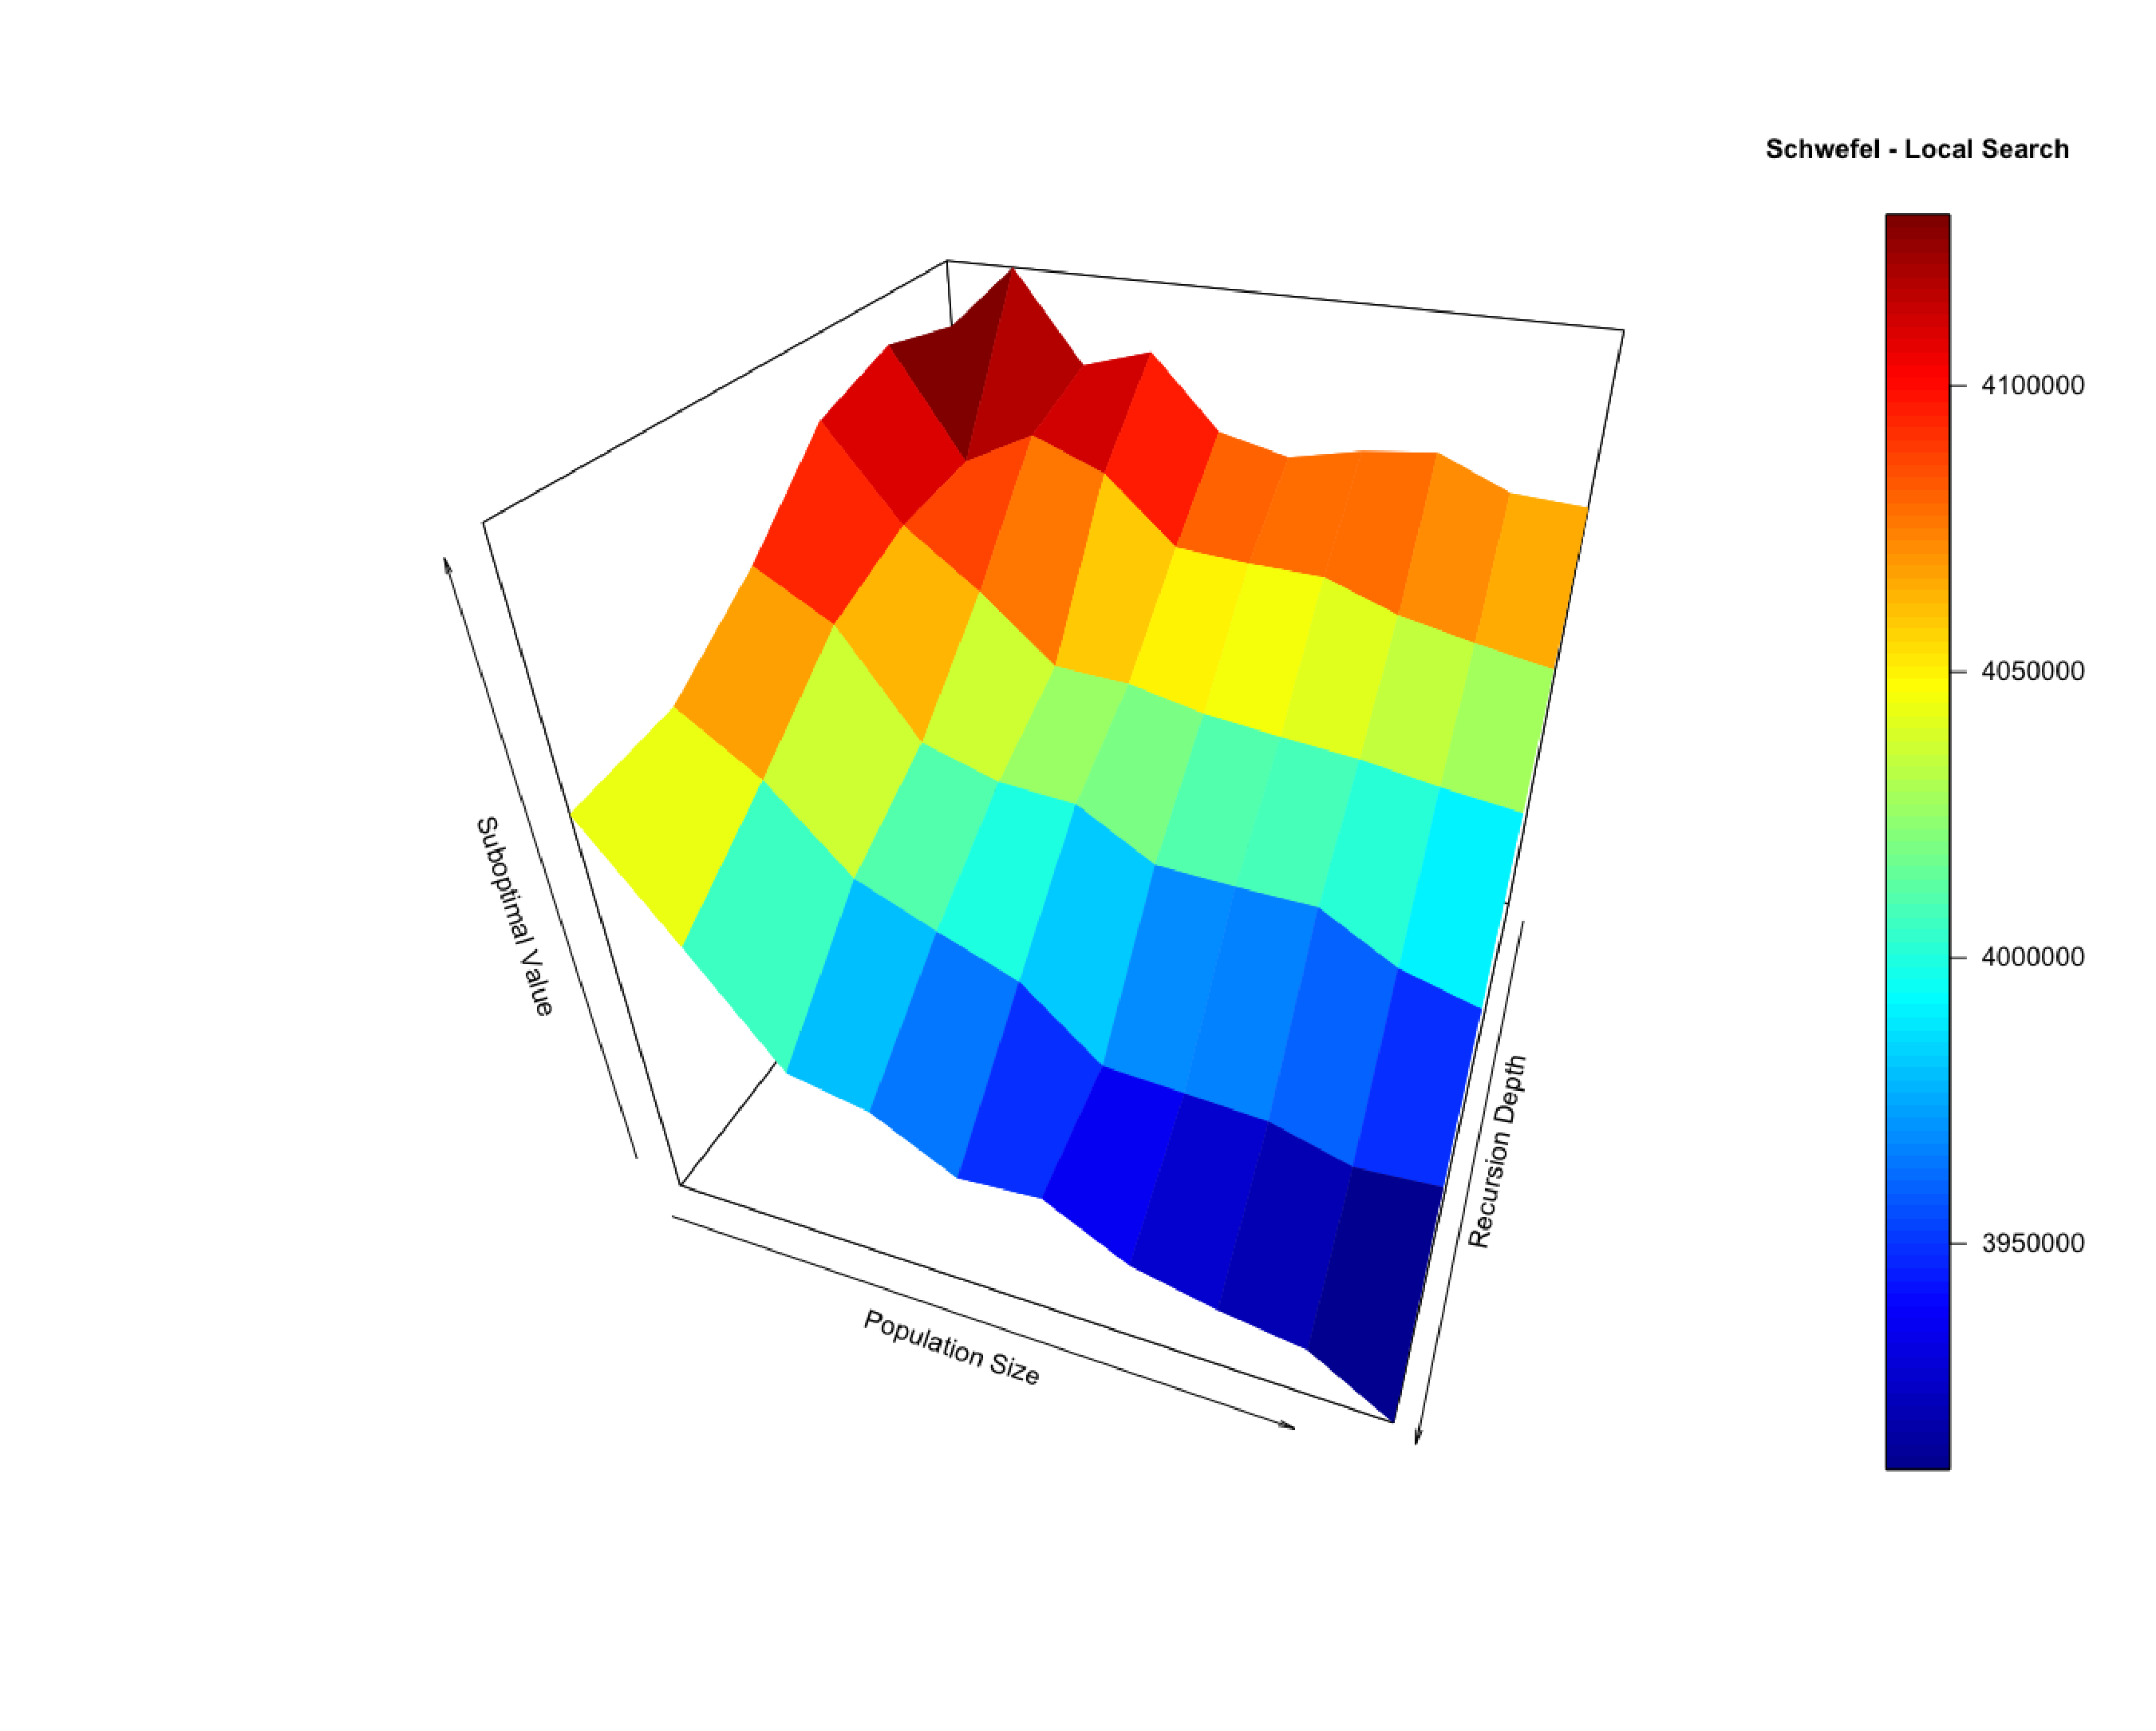
\includegraphics[width=1.0\hsize,height=0.65\hsize]{fig09.eps}
\caption{Schwefel - Local Search - Suboptimal Values}
\label{fig03}
\end{figure}

\begin{figure}[tbp]
\centering
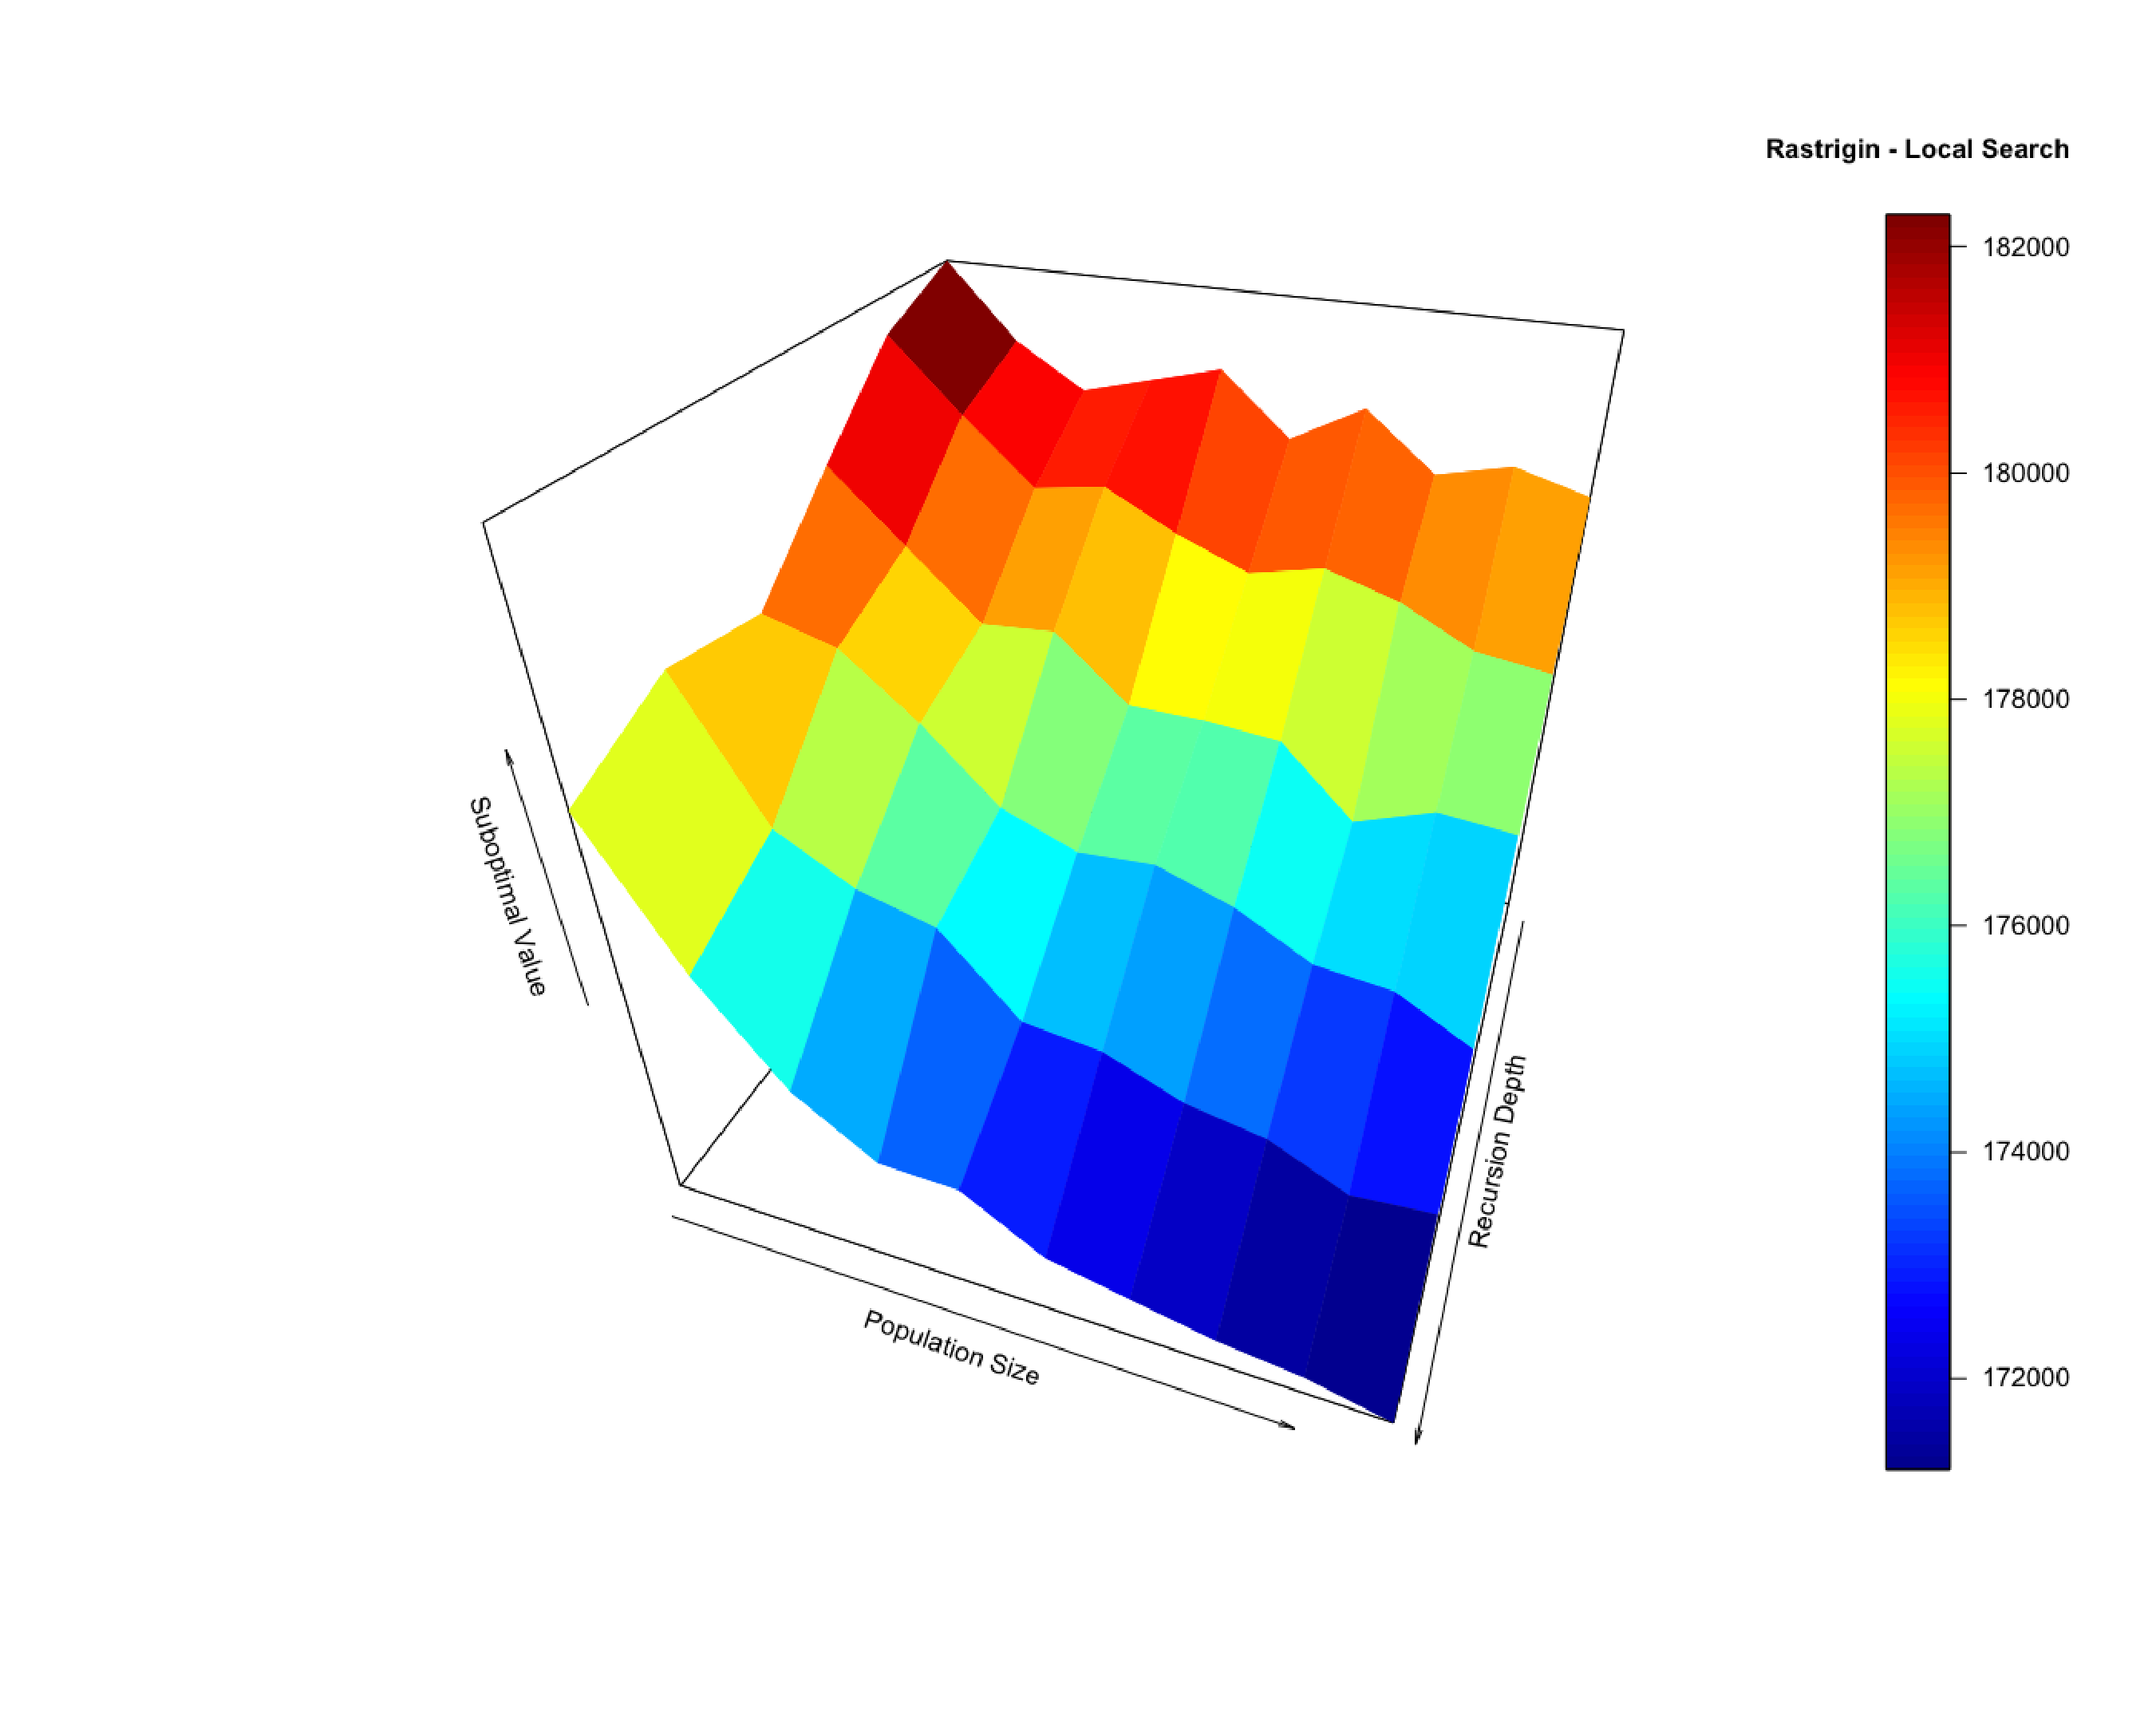
\includegraphics[width=1.0\hsize,height=0.65\hsize]{fig12.eps}
\caption{Rastrigin - Local Search - Suboptimal Values}
\label{fig04}
\end{figure}

\begin{figure}[tbp]
\centering
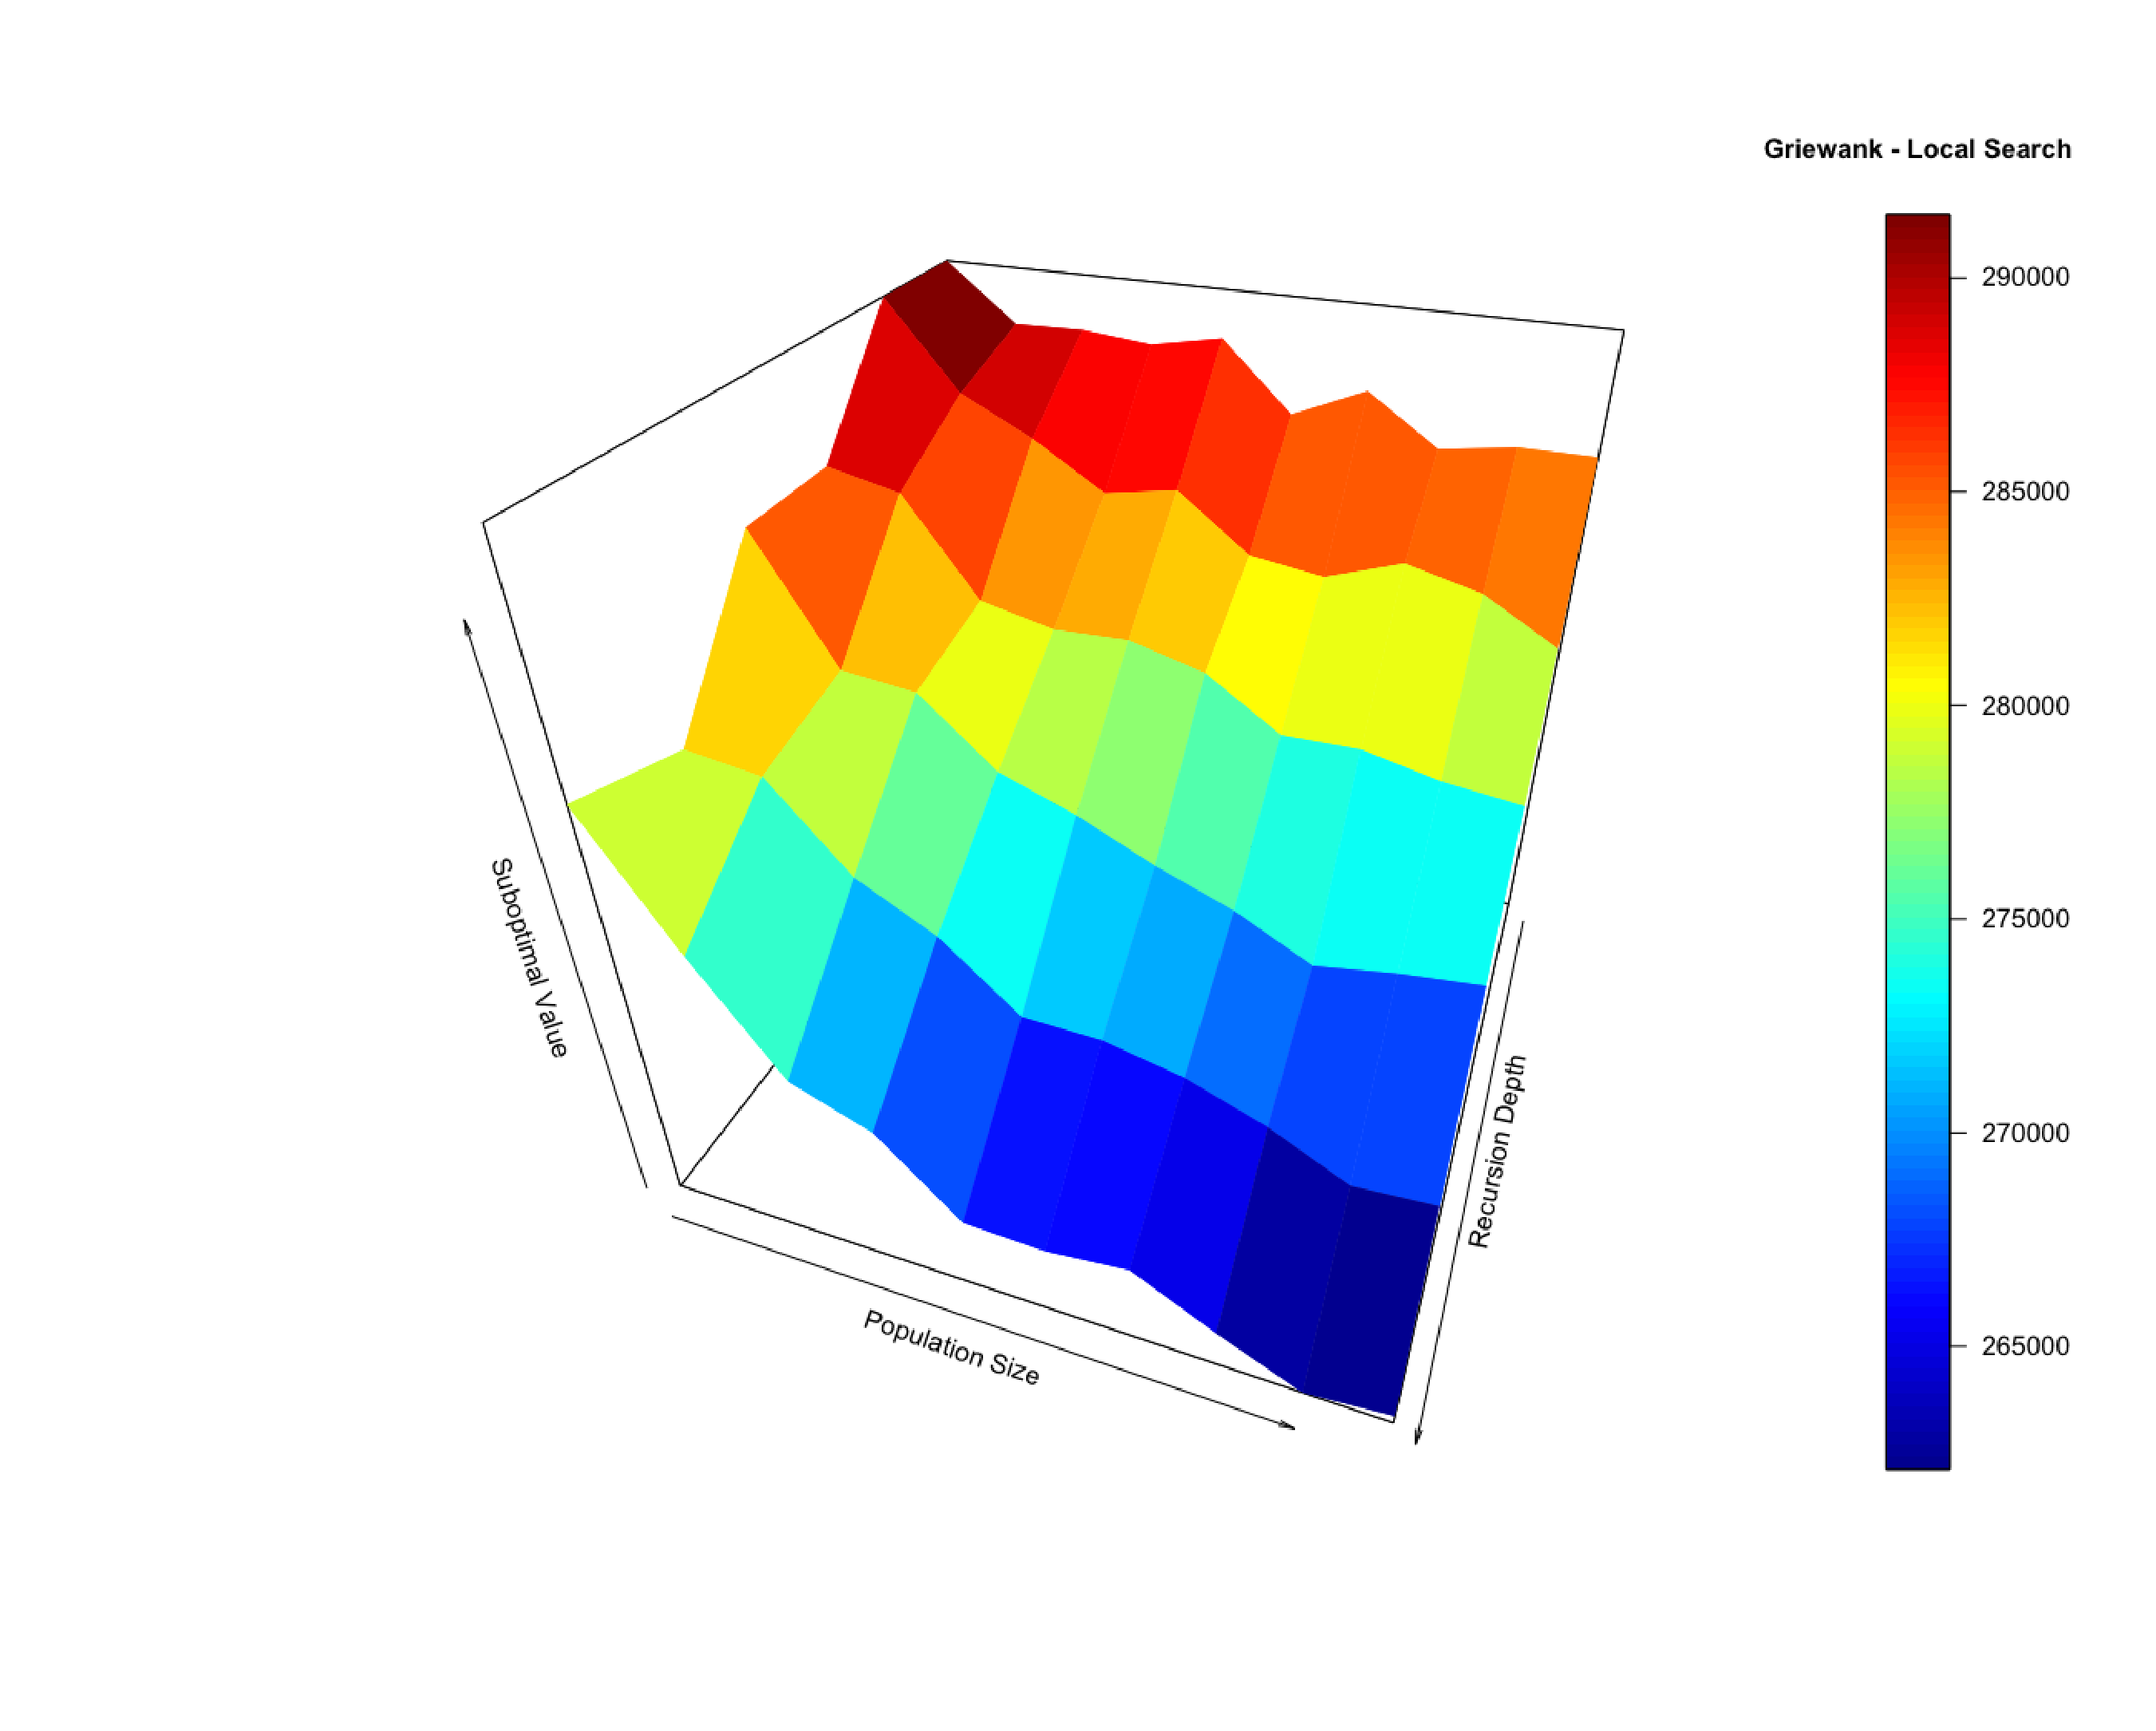
\includegraphics[width=1.0\hsize,height=0.65\hsize]{fig15.eps}
\caption{Griewank - Local Search - Suboptimal Values}
\label{fig05}
\end{figure}

\begin{figure}[tbp]
\centering
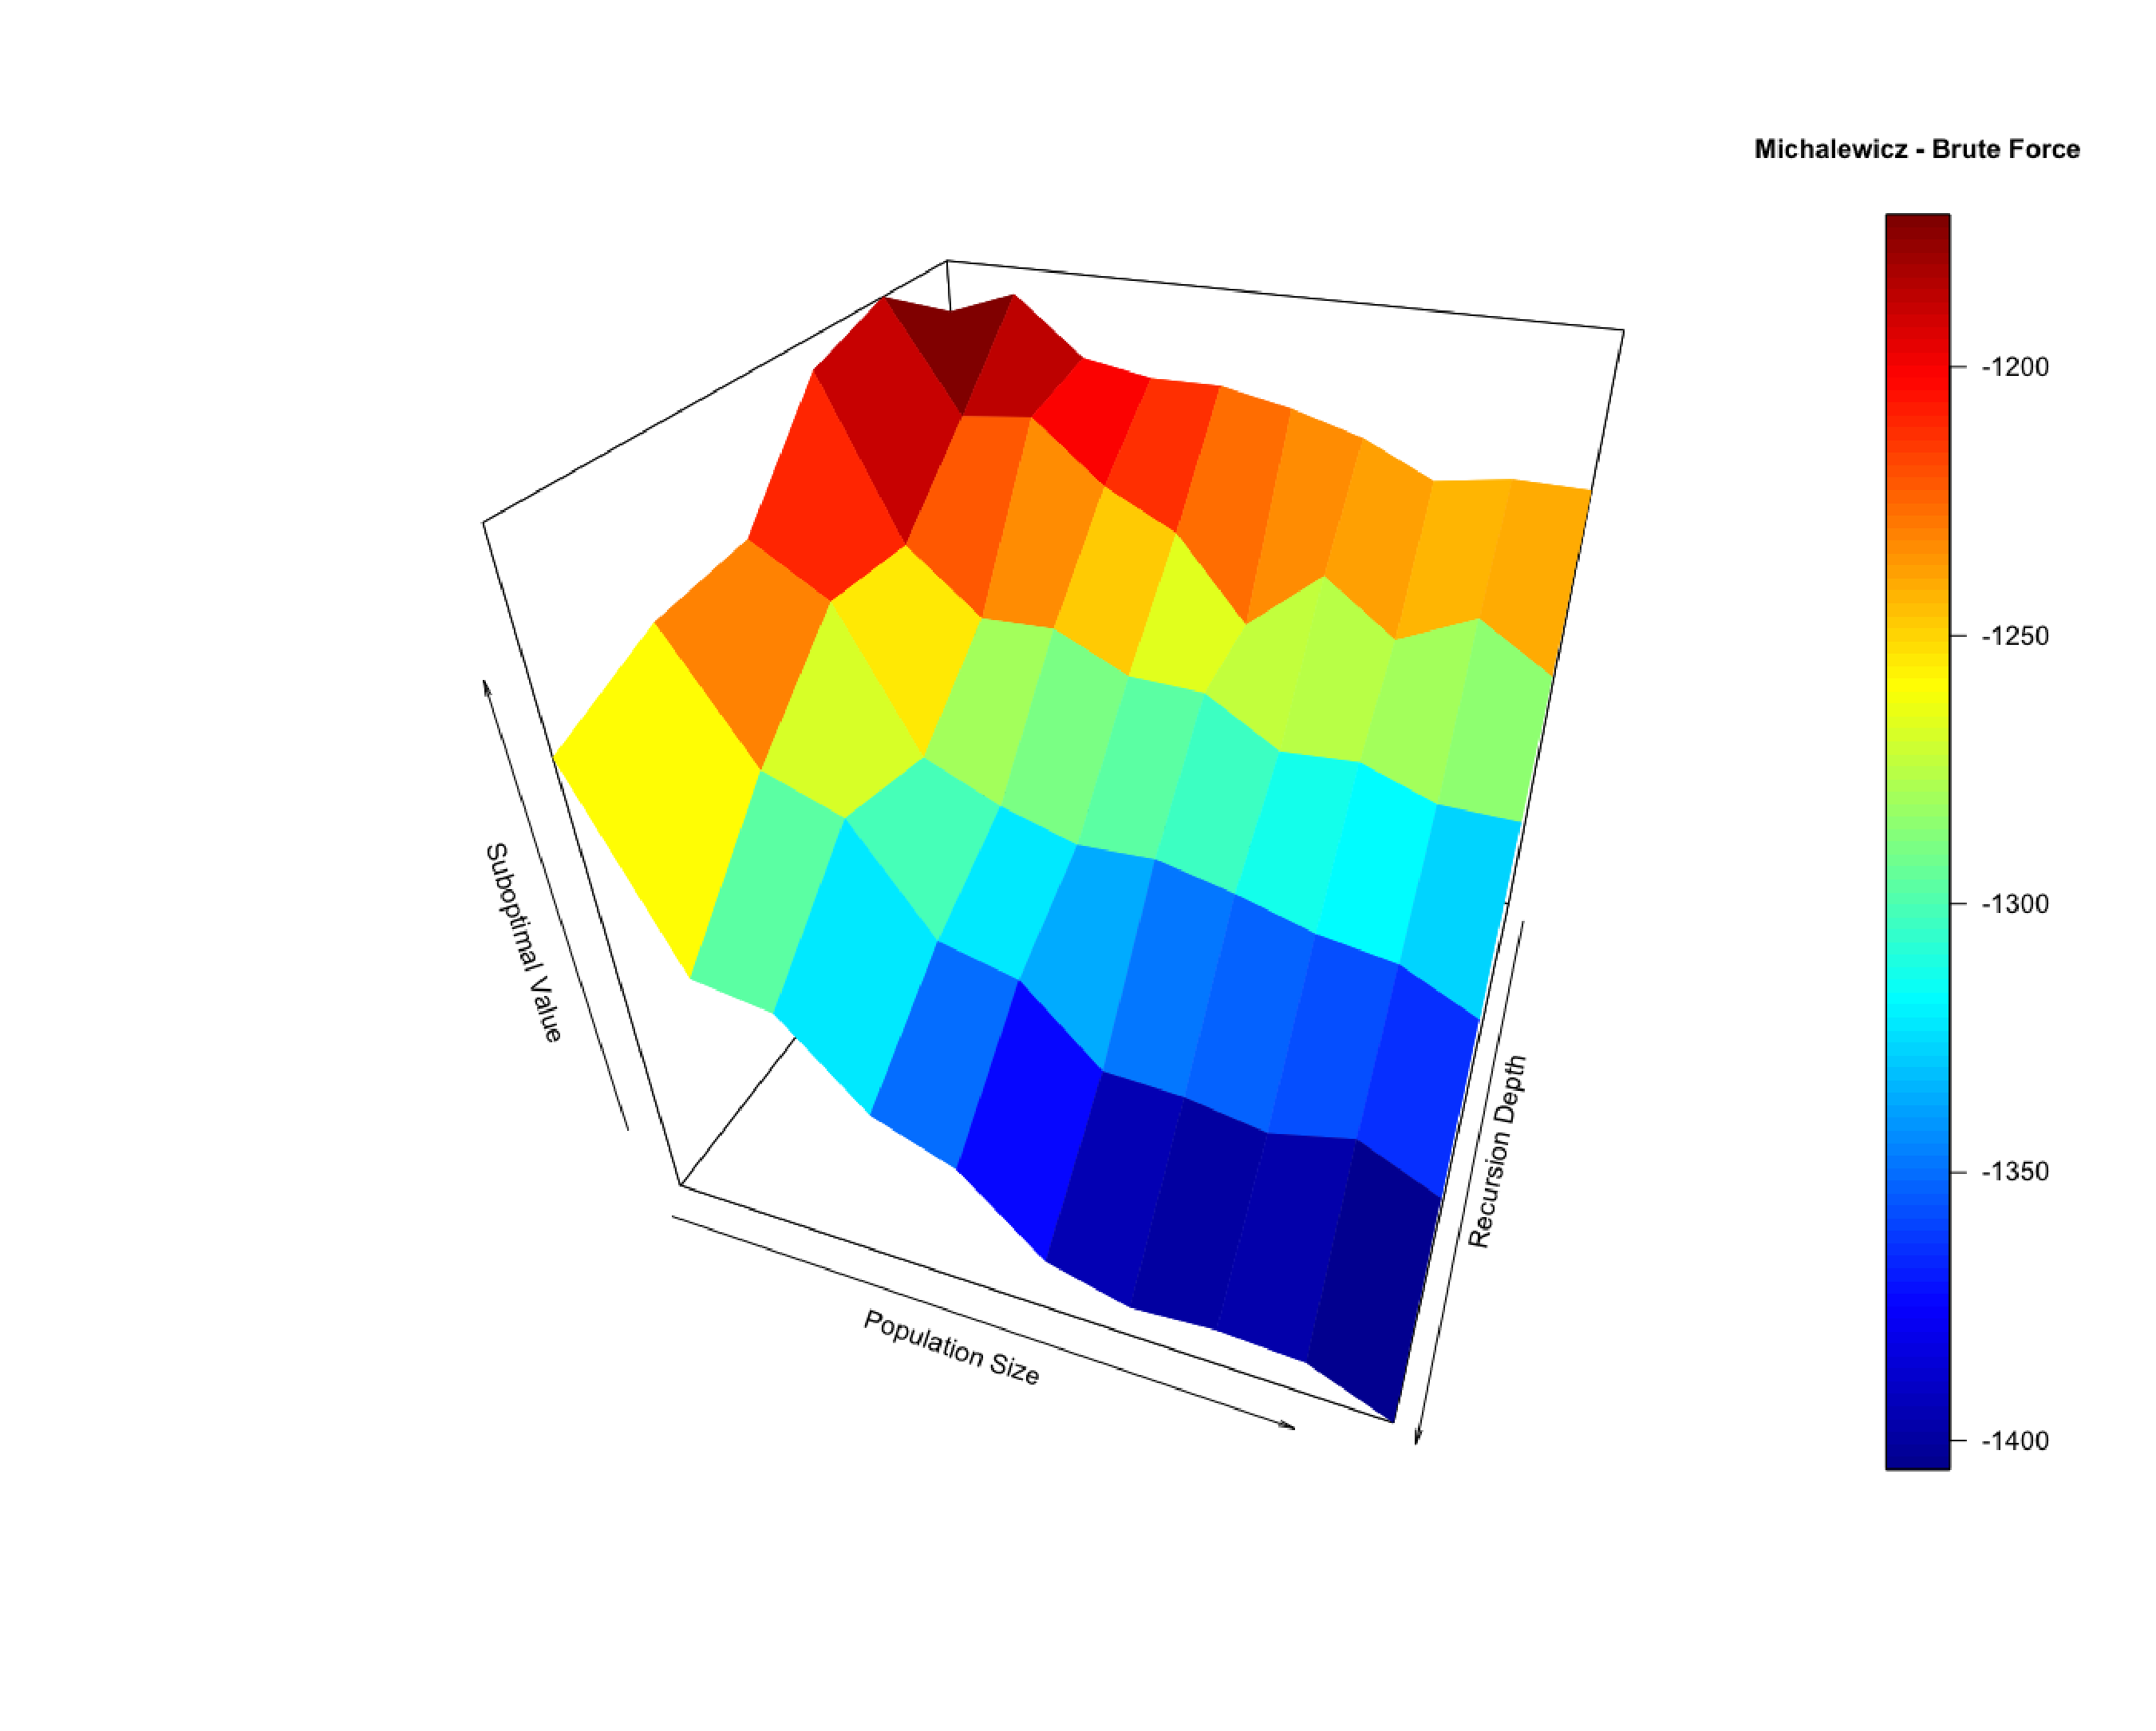
\includegraphics[width=1.0\hsize,height=0.65\hsize]{fig18.eps}
\caption{Michalewicz - Brute Force - Suboptimal Values}
\label{fig06}
\end{figure}

\begin{figure}[tbp]
\centering
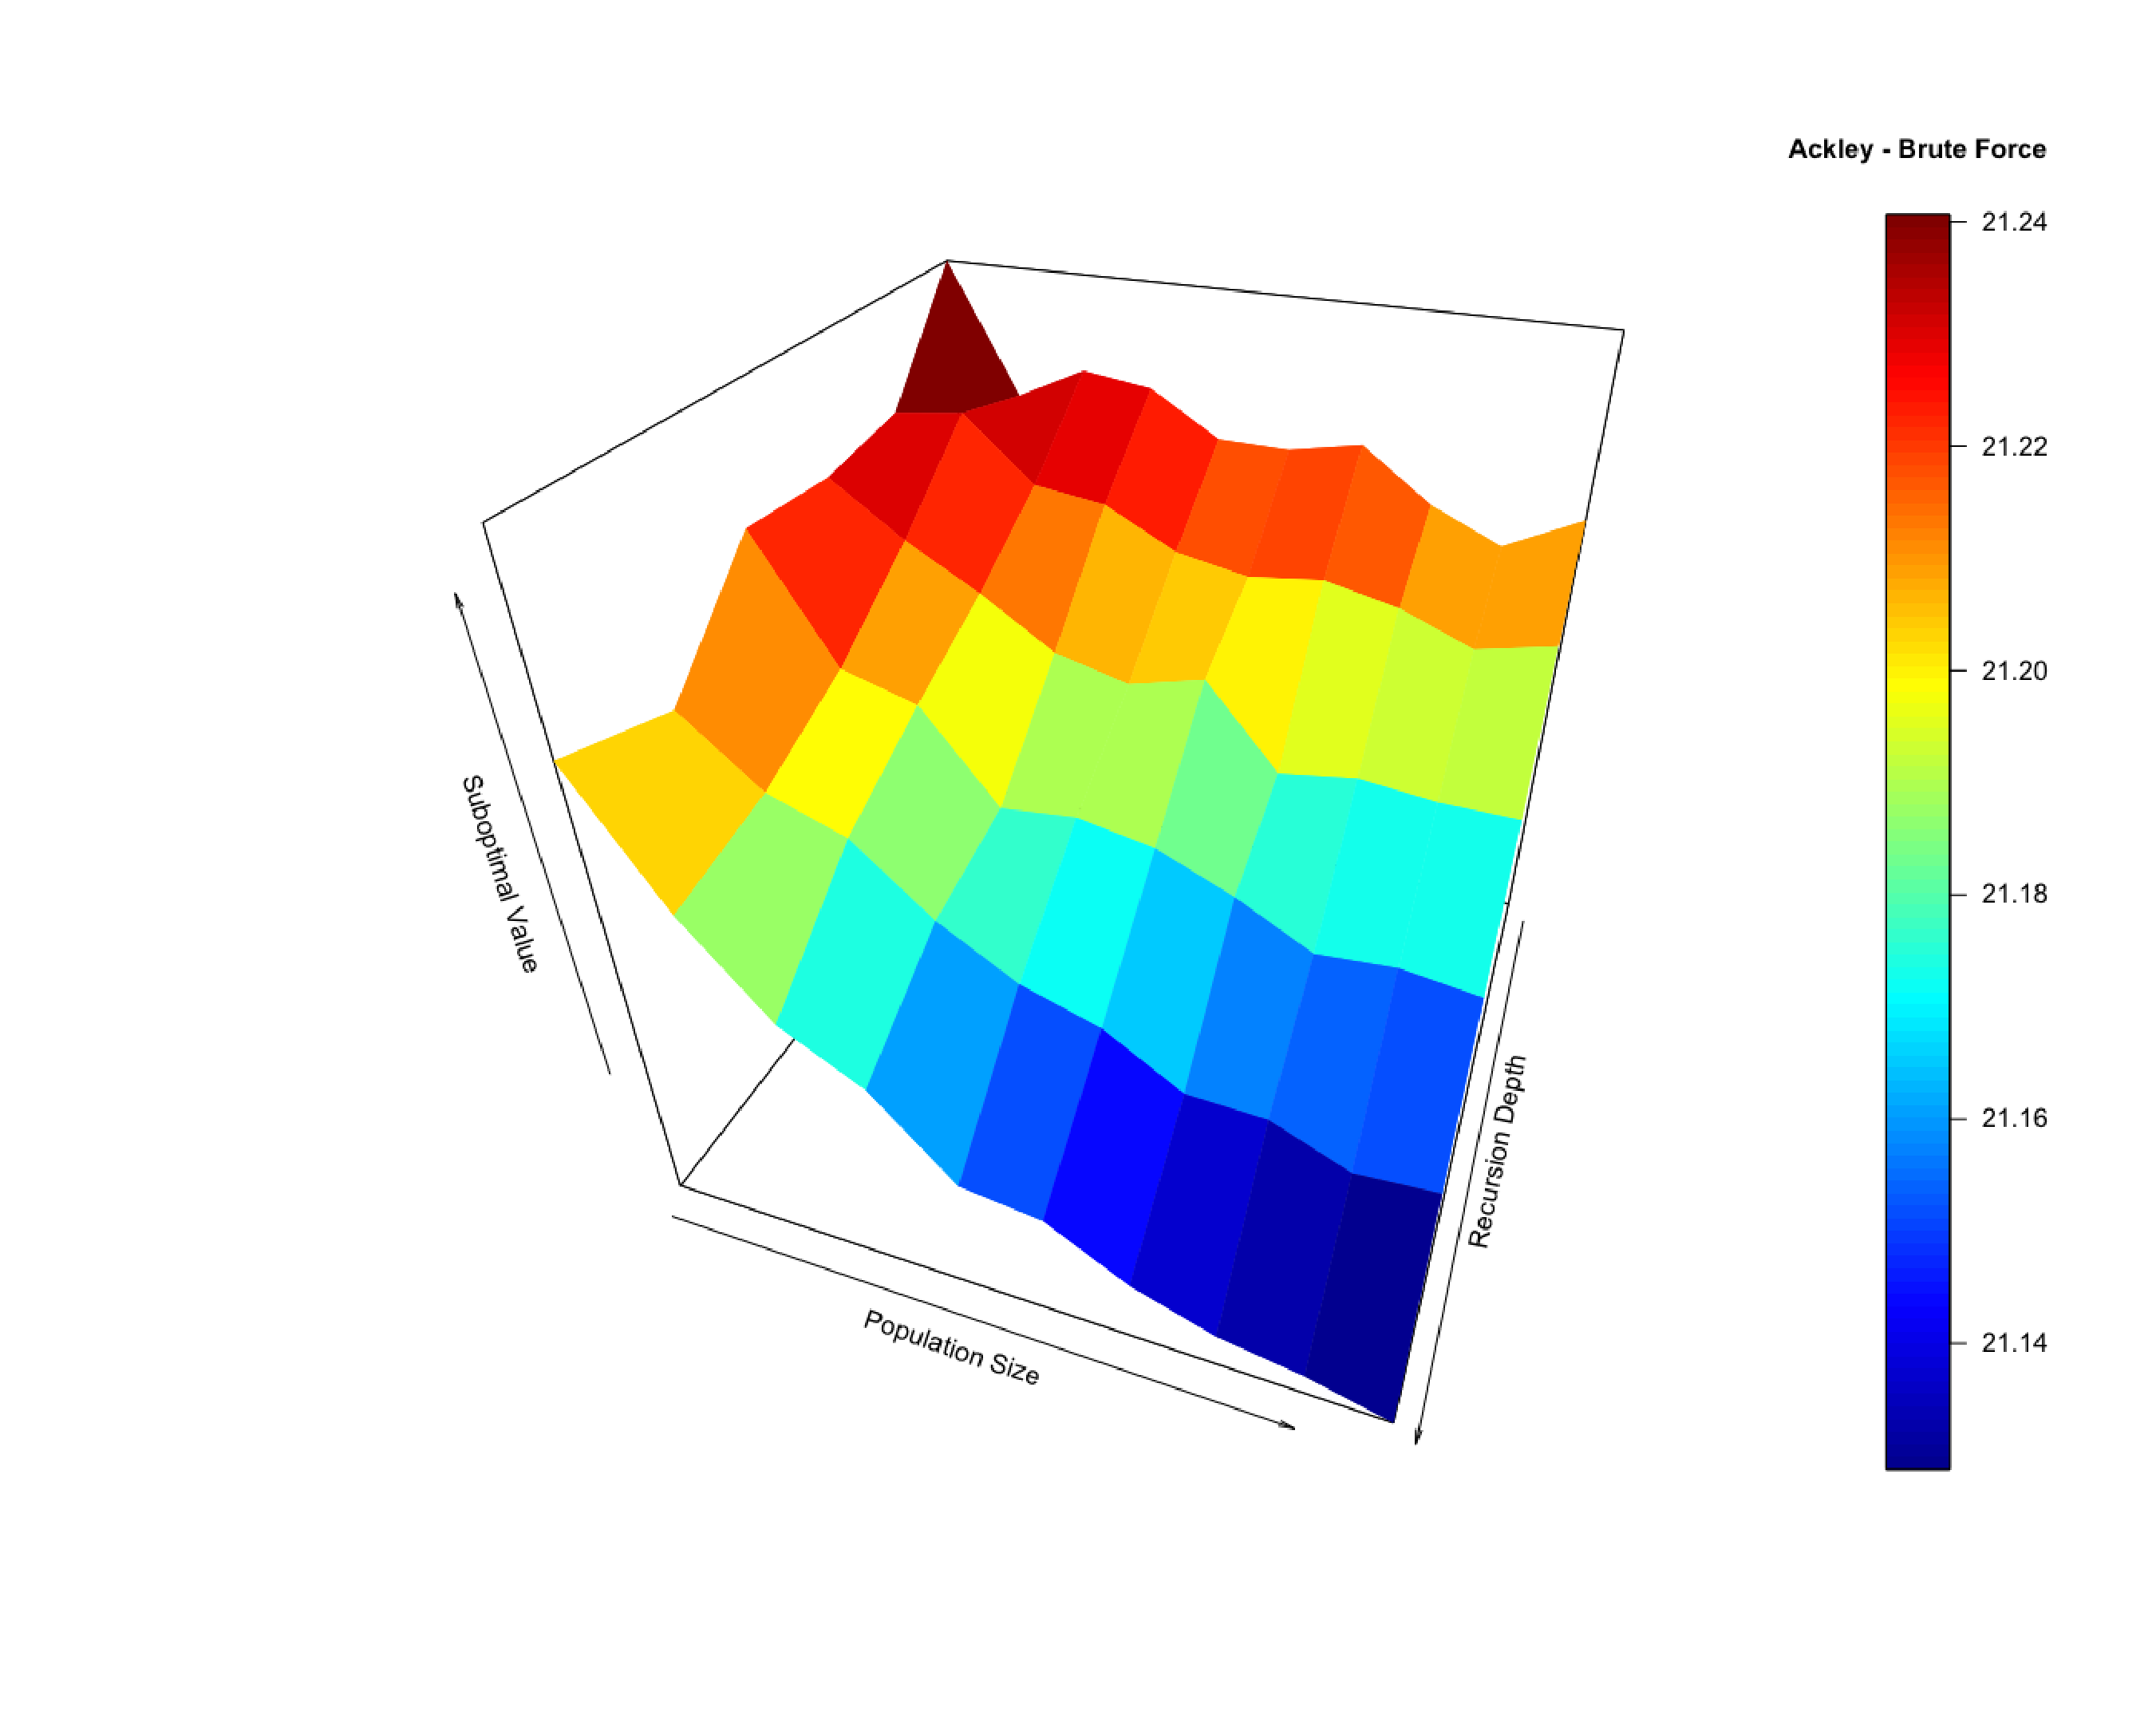
\includegraphics[width=1.0\hsize,height=0.65\hsize]{fig21.eps}
\caption{Ackley - Brute Force - Suboptimal Values}
\label{fig07}
\end{figure}

\begin{figure}[tbp]
\centering
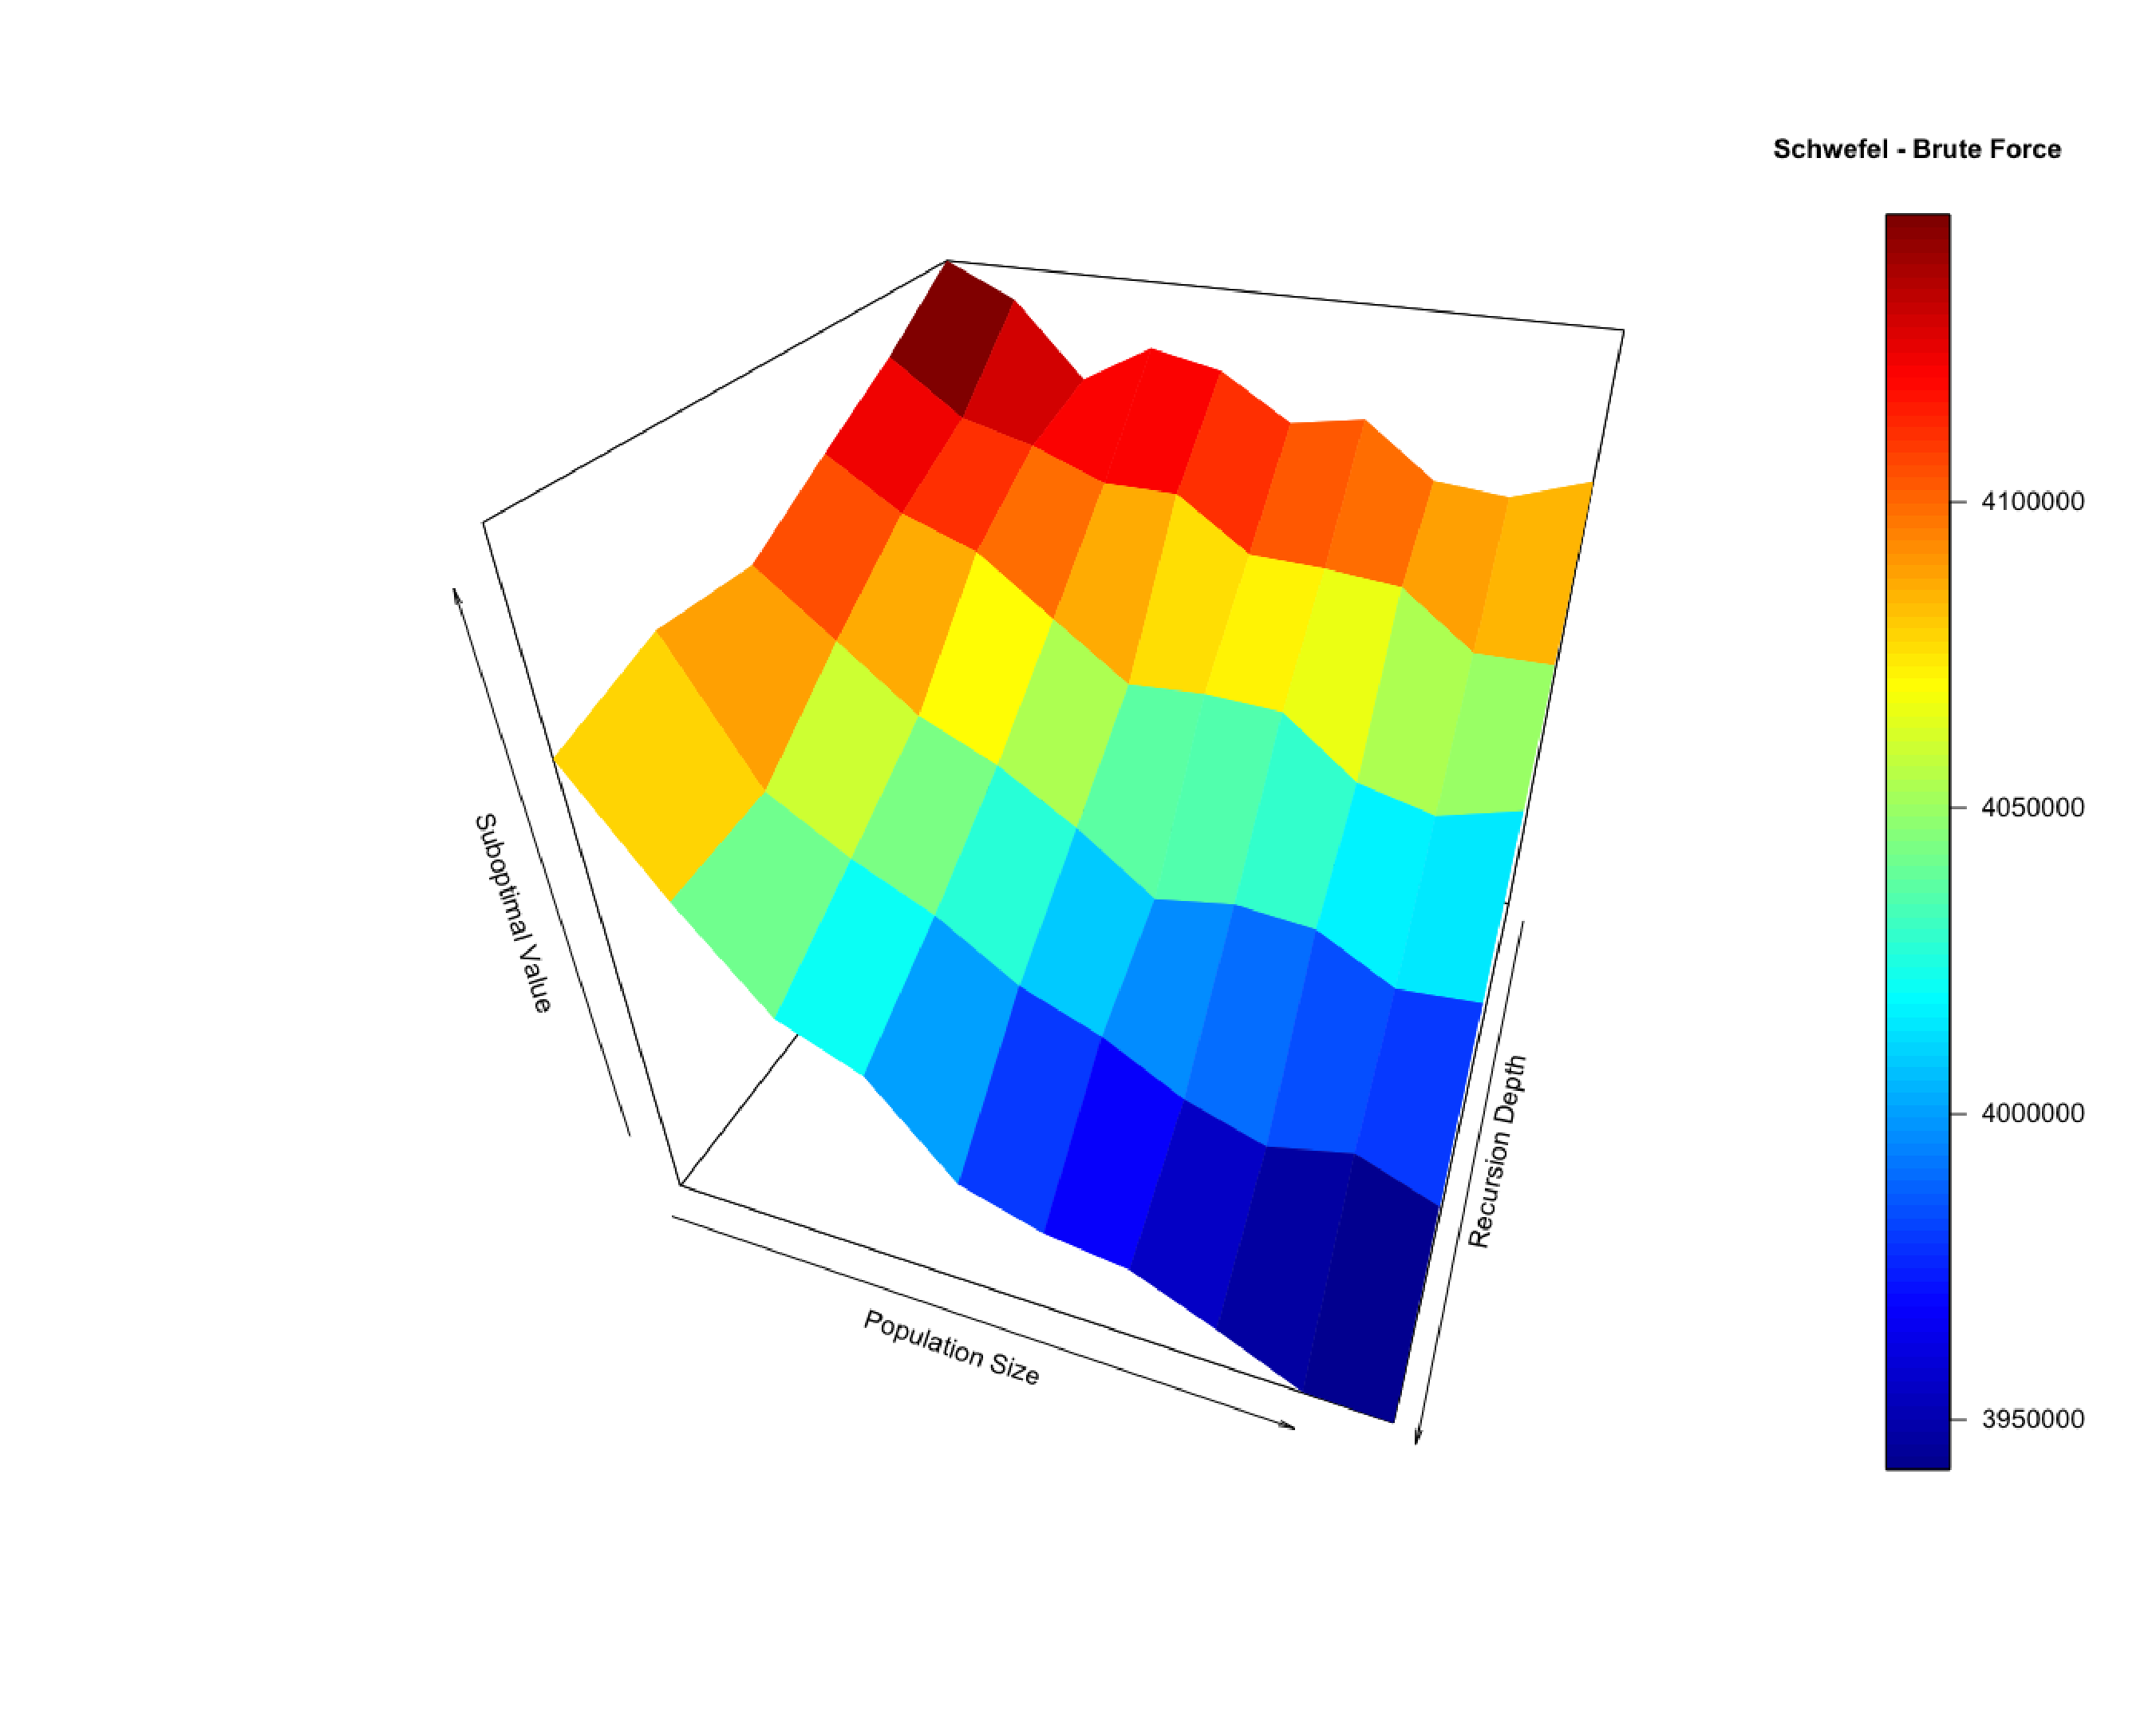
\includegraphics[width=1.0\hsize,height=0.65\hsize]{fig24.eps}
\caption{Schwefel - Brute Force - Suboptimal Values}
\label{fig08}
\end{figure}

\begin{figure}[tbp]
\centering
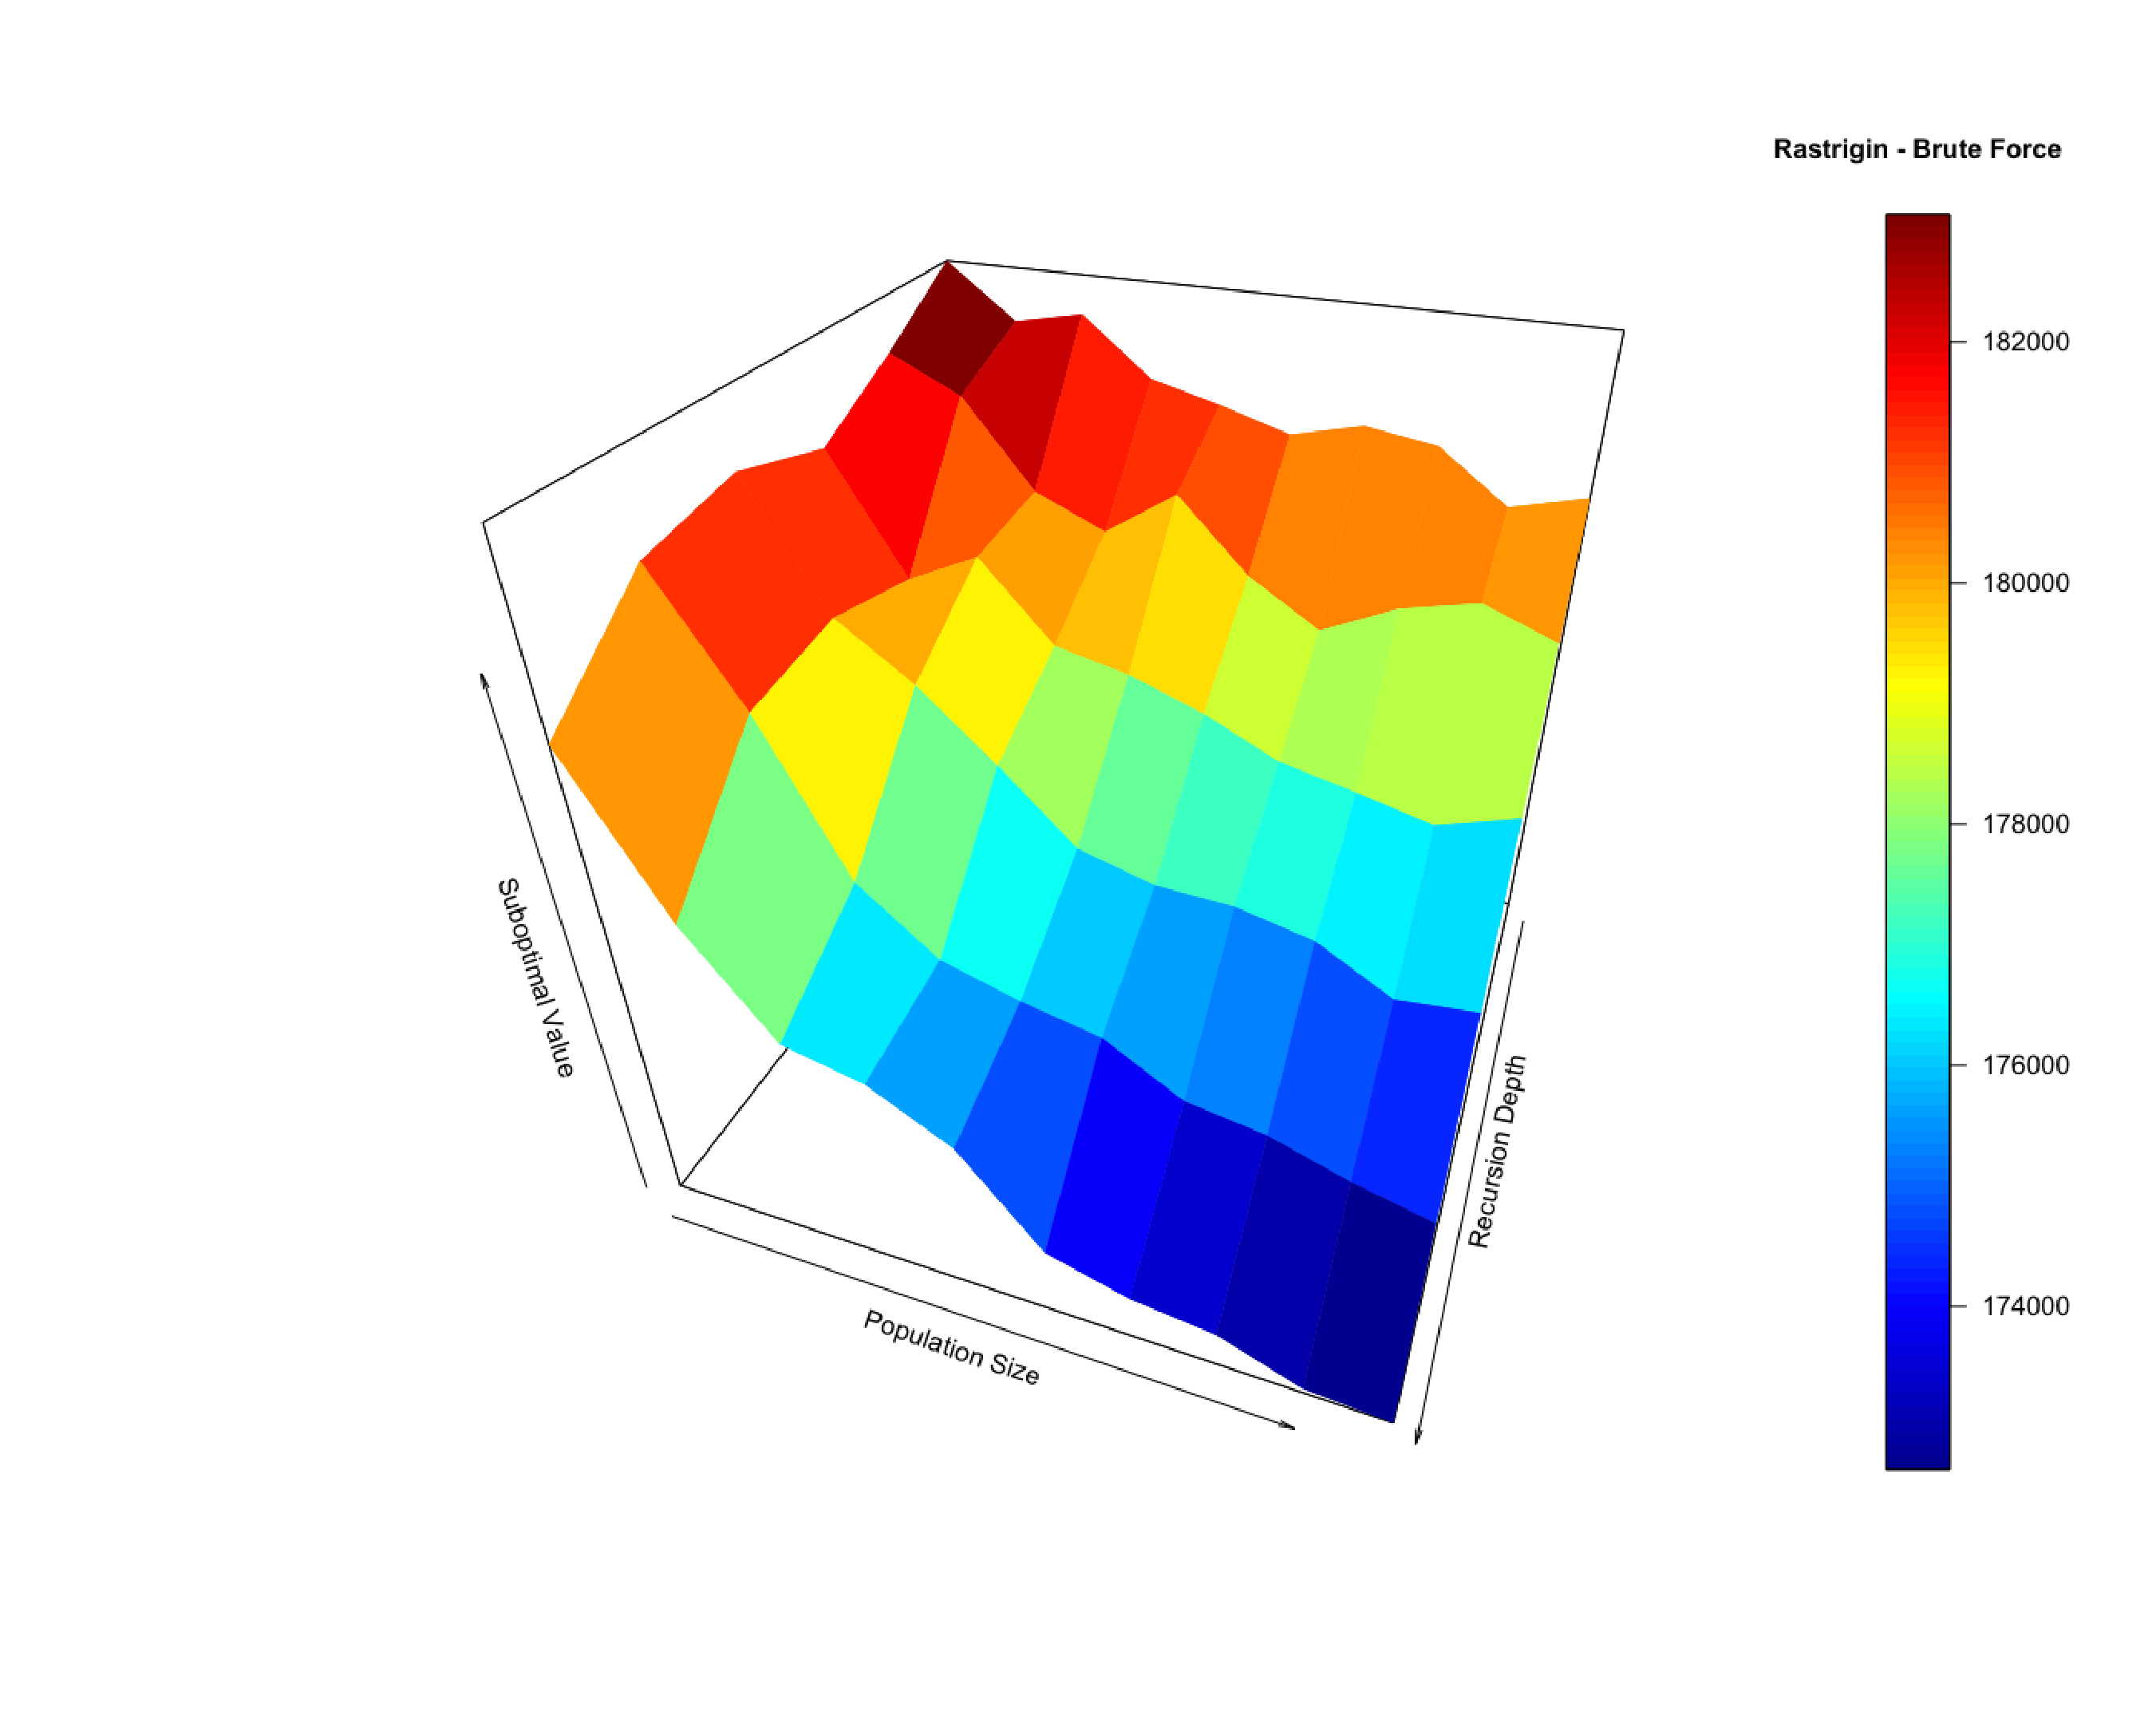
\includegraphics[width=1.0\hsize,height=0.65\hsize]{fig27.eps}
\caption{Rastrigin - Brute Force - Suboptimal Values}
\label{fig09}
\end{figure}

\begin{figure}[tbp]
\centering
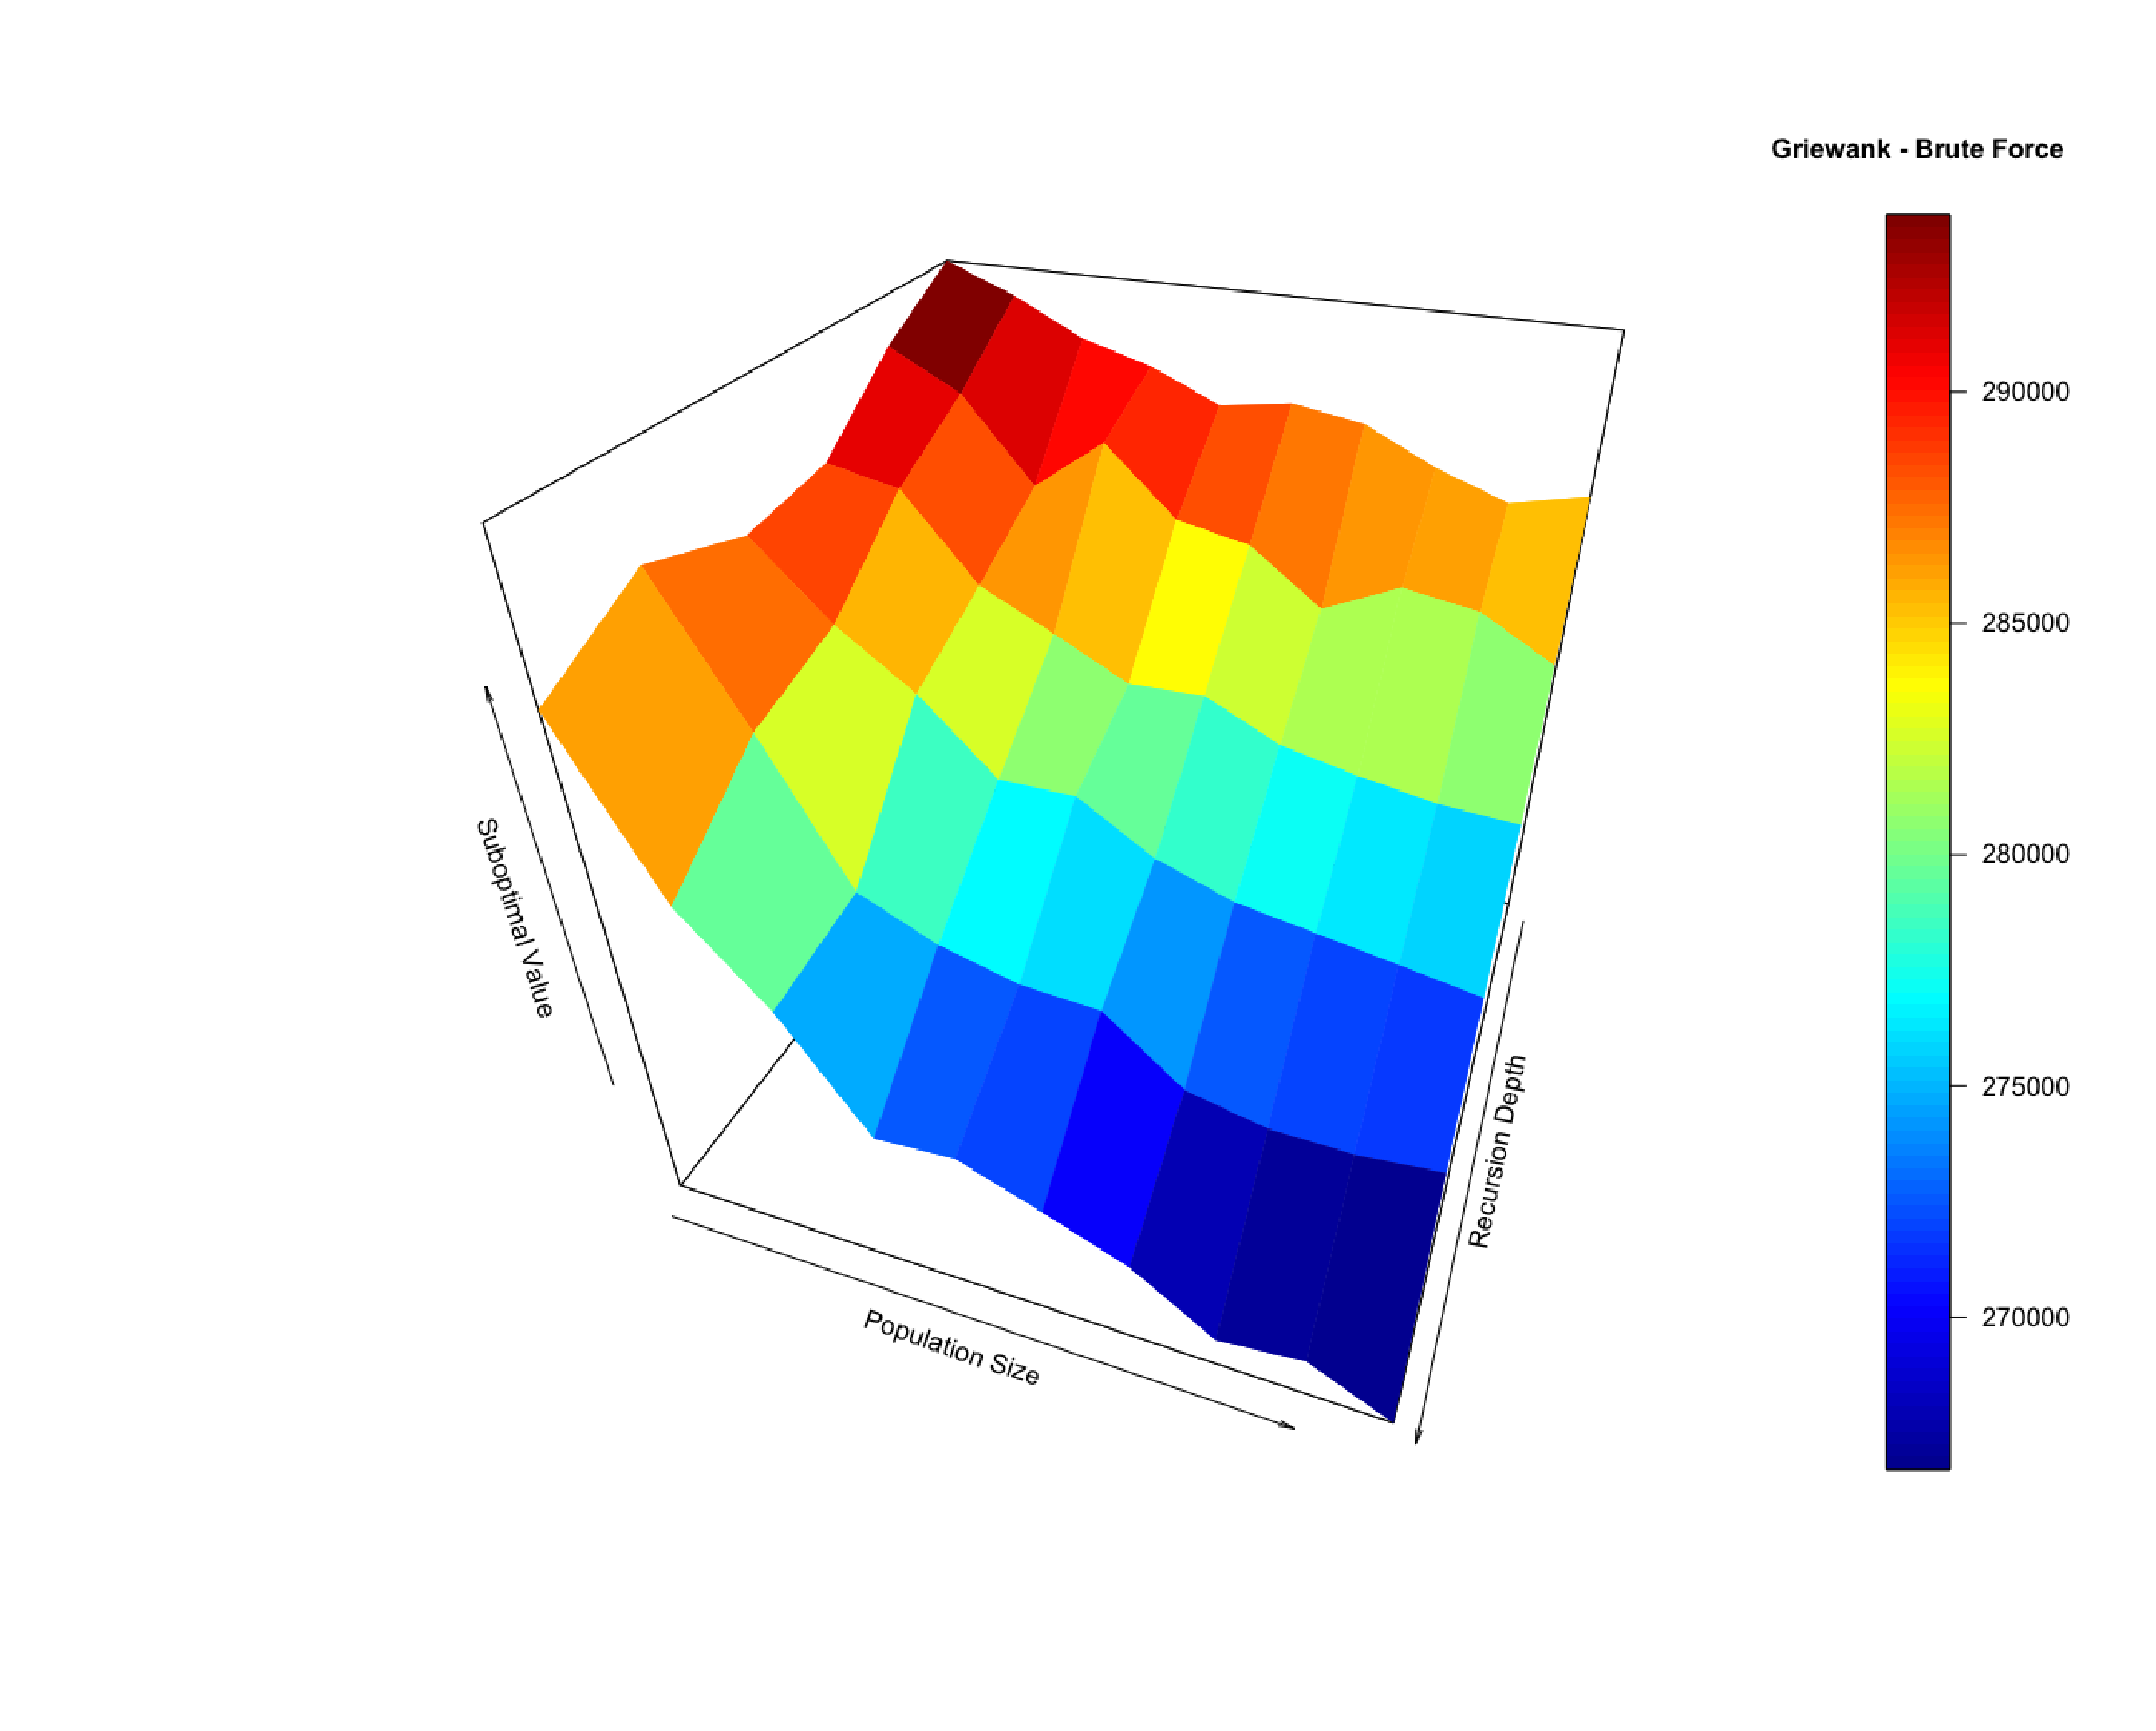
\includegraphics[width=1.0\hsize,height=0.65\hsize]{fig30.eps}
\caption{Griewank - Brute Force - Suboptimal Values}
\label{fig10}
\end{figure}

\begin{figure}[tbp]
\centering
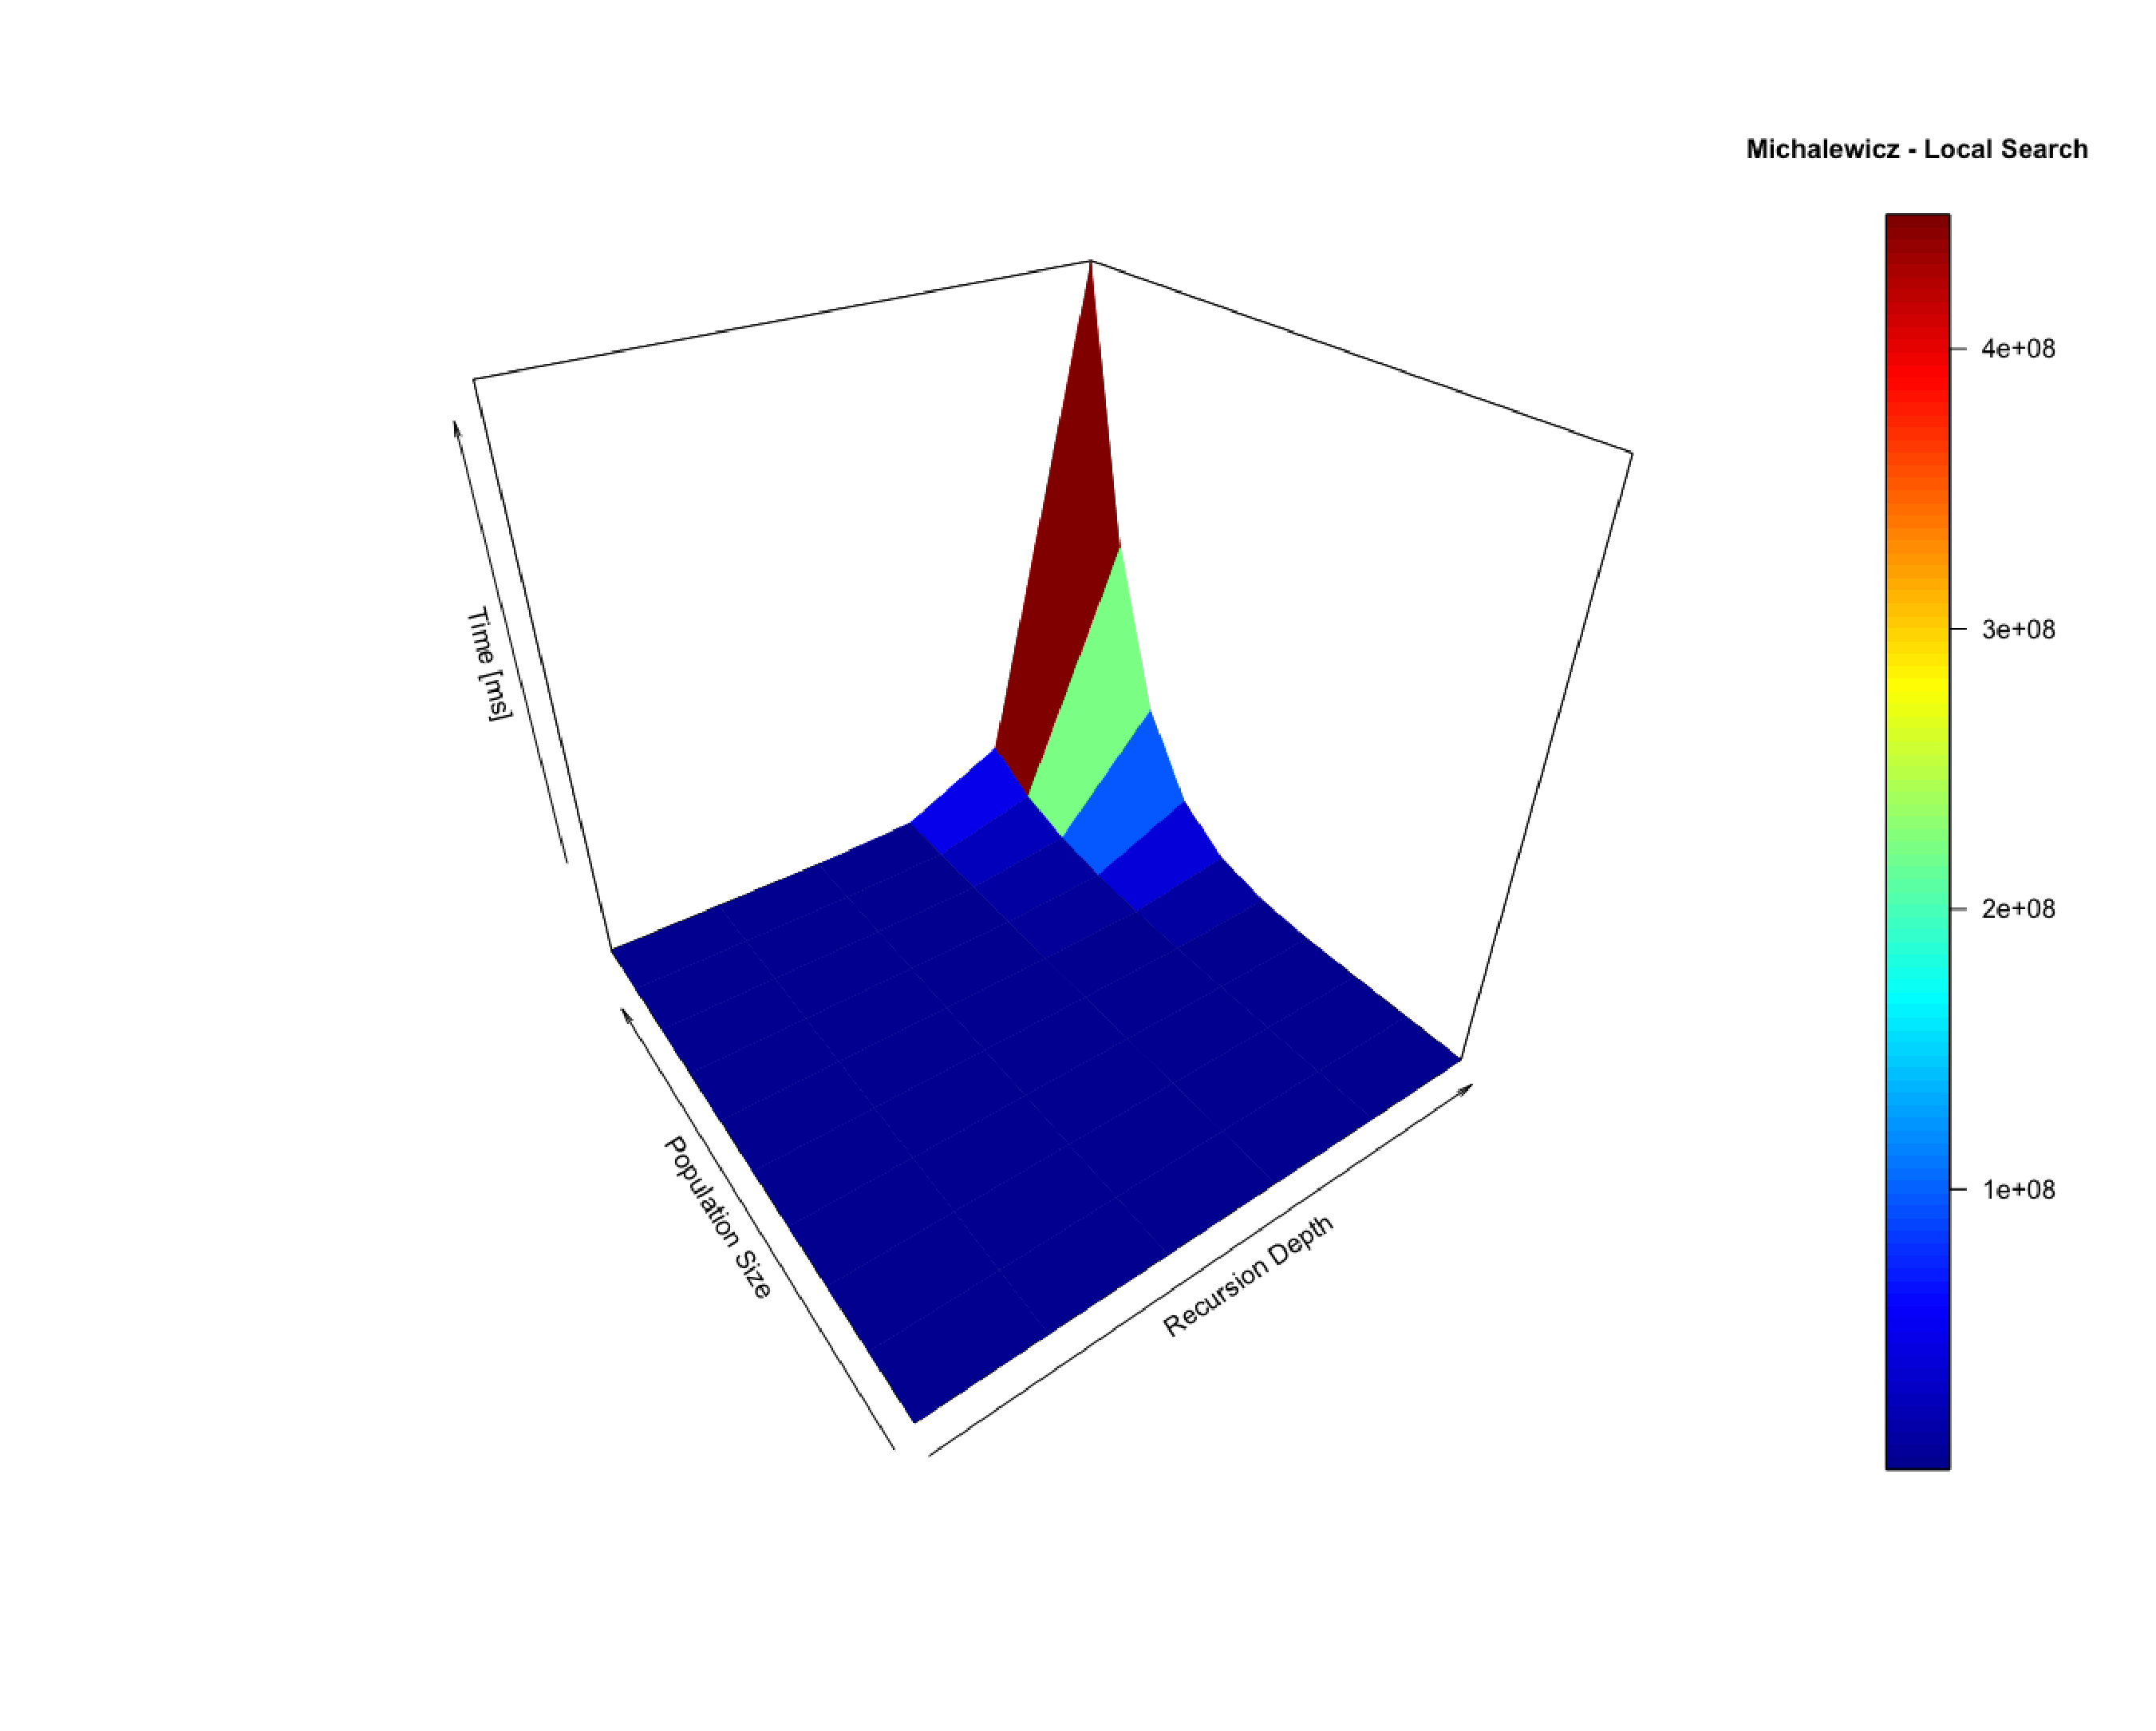
\includegraphics[width=1.0\hsize,height=0.65\hsize]{fig02.eps}
\caption{Michalewicz - Local Search - Time[ms]}
\label{fig11}
\end{figure}

\begin{figure}[tbp]
\centering
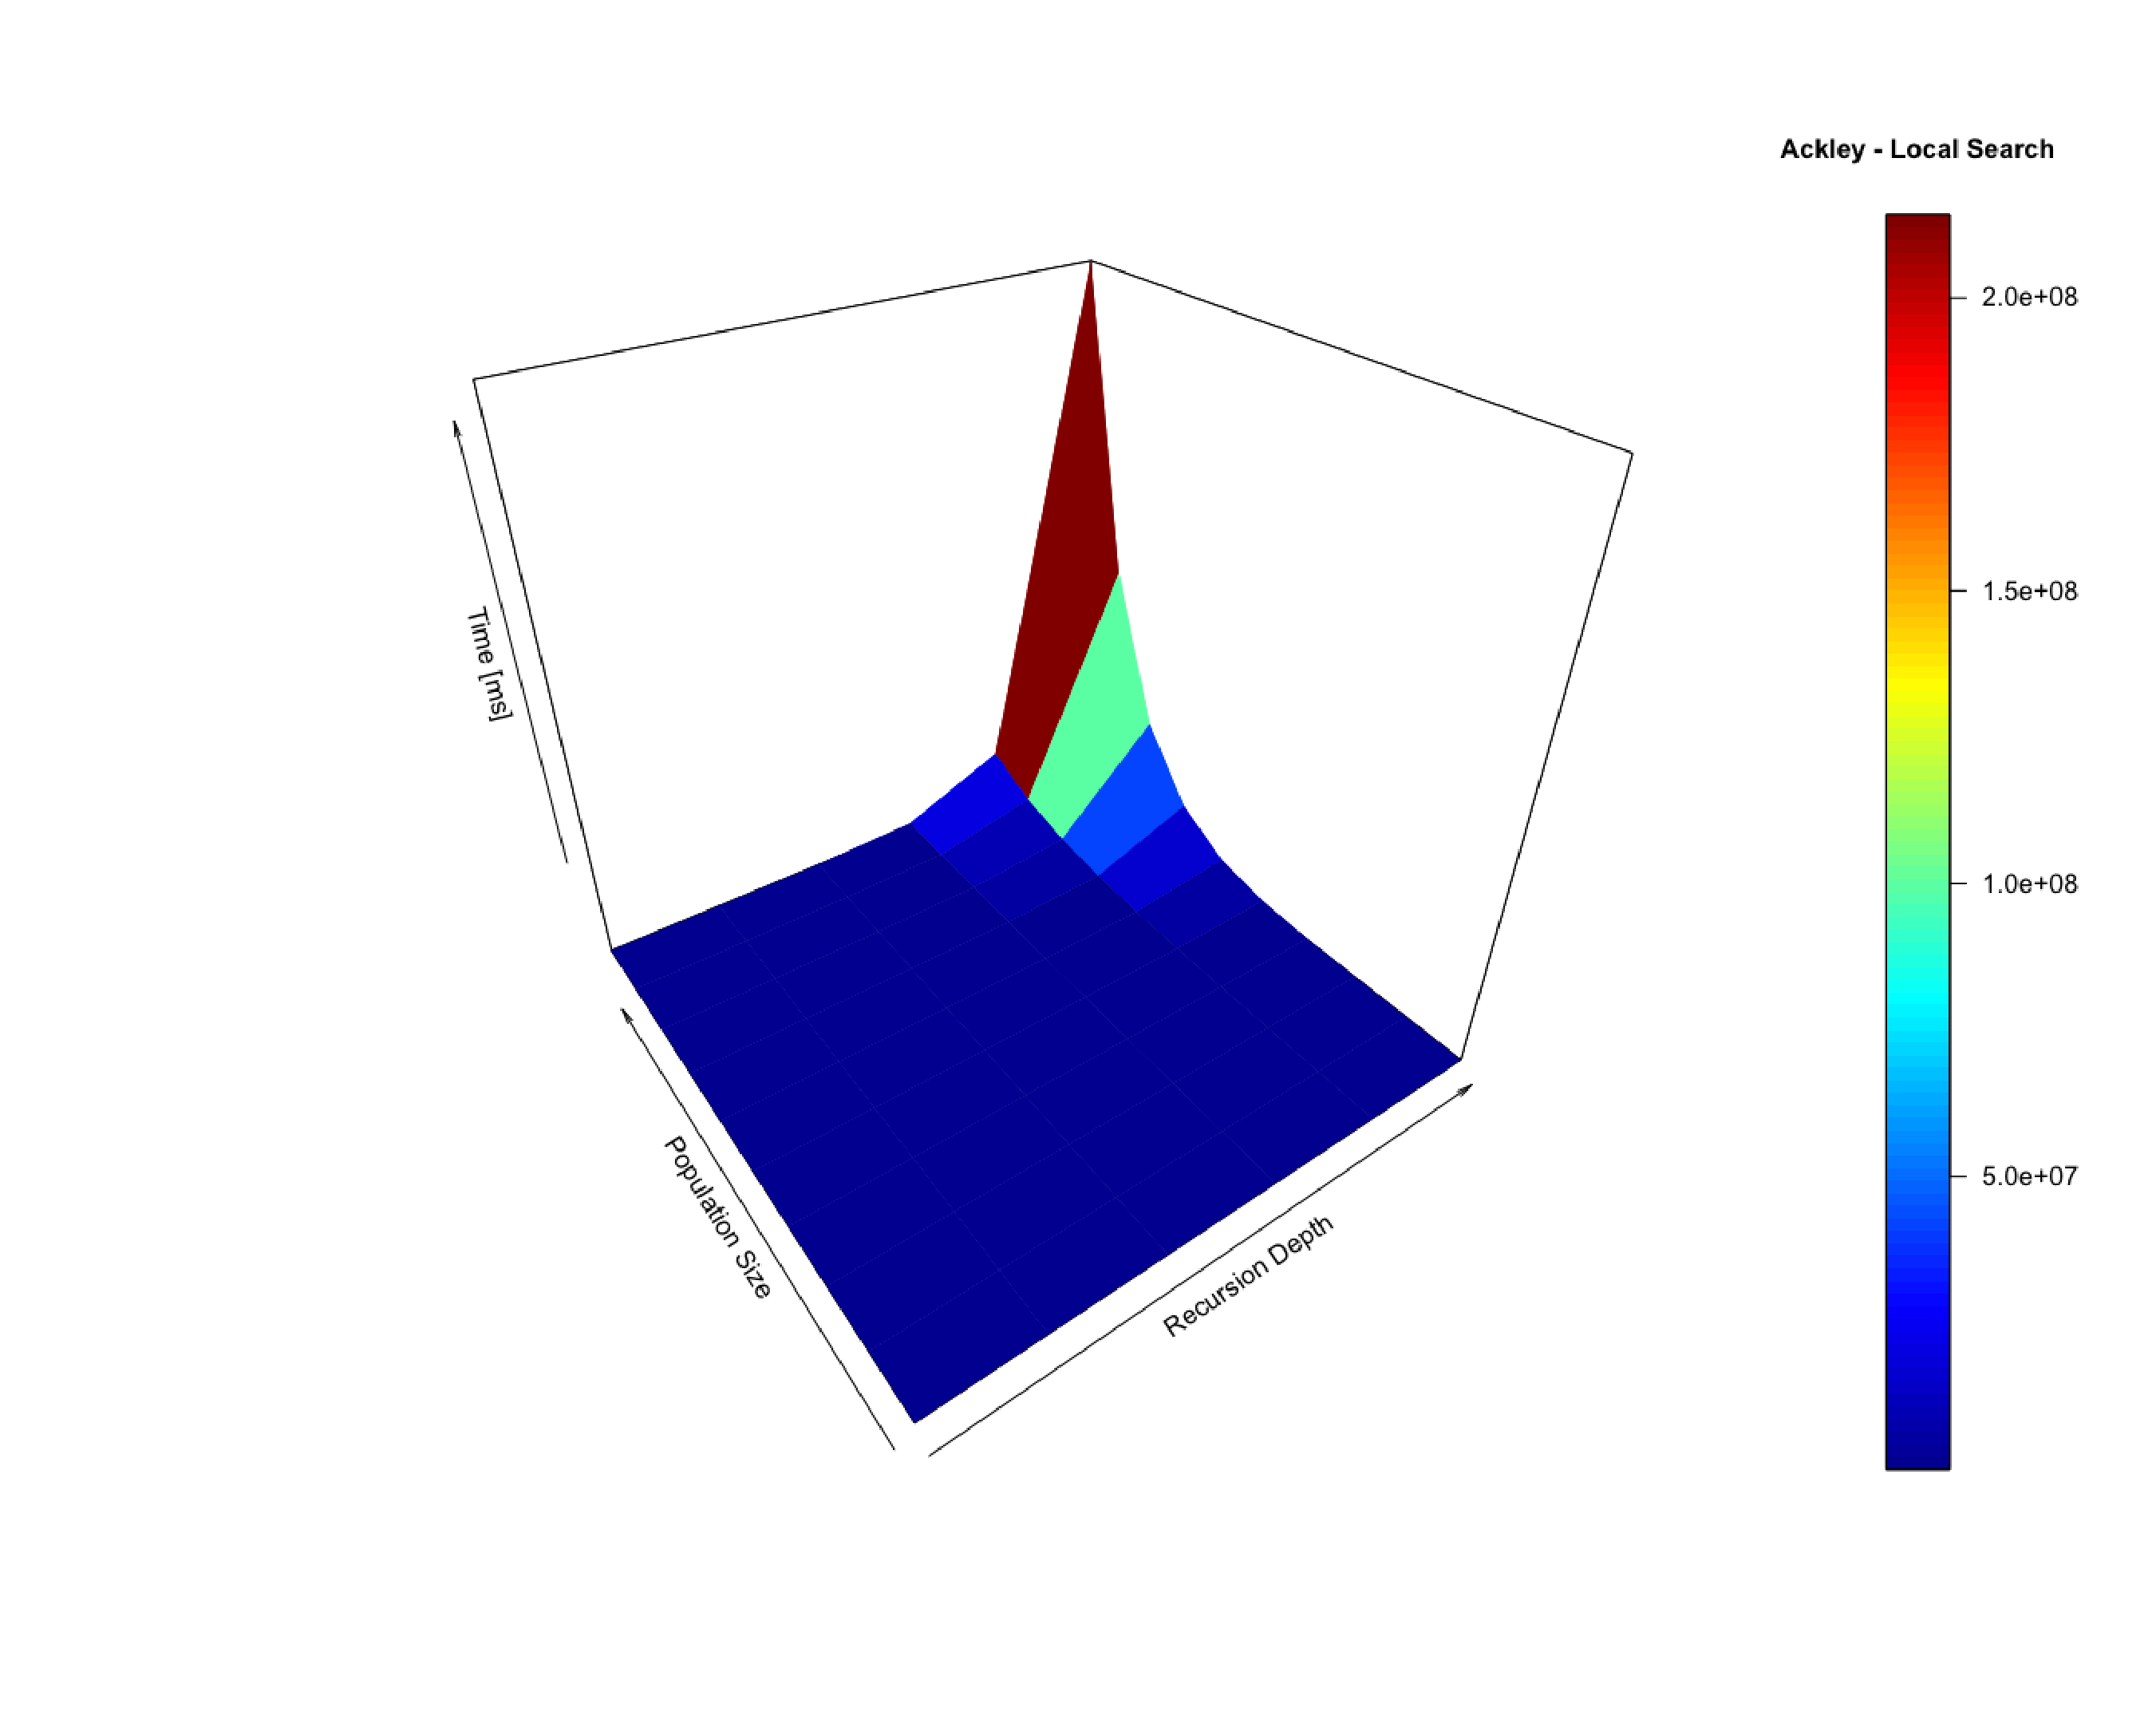
\includegraphics[width=1.0\hsize,height=0.65\hsize]{fig05.eps}
\caption{Ackley - Local Search - Time[ms]}
\label{fig12}
\end{figure}

\begin{figure}[tbp]
\centering
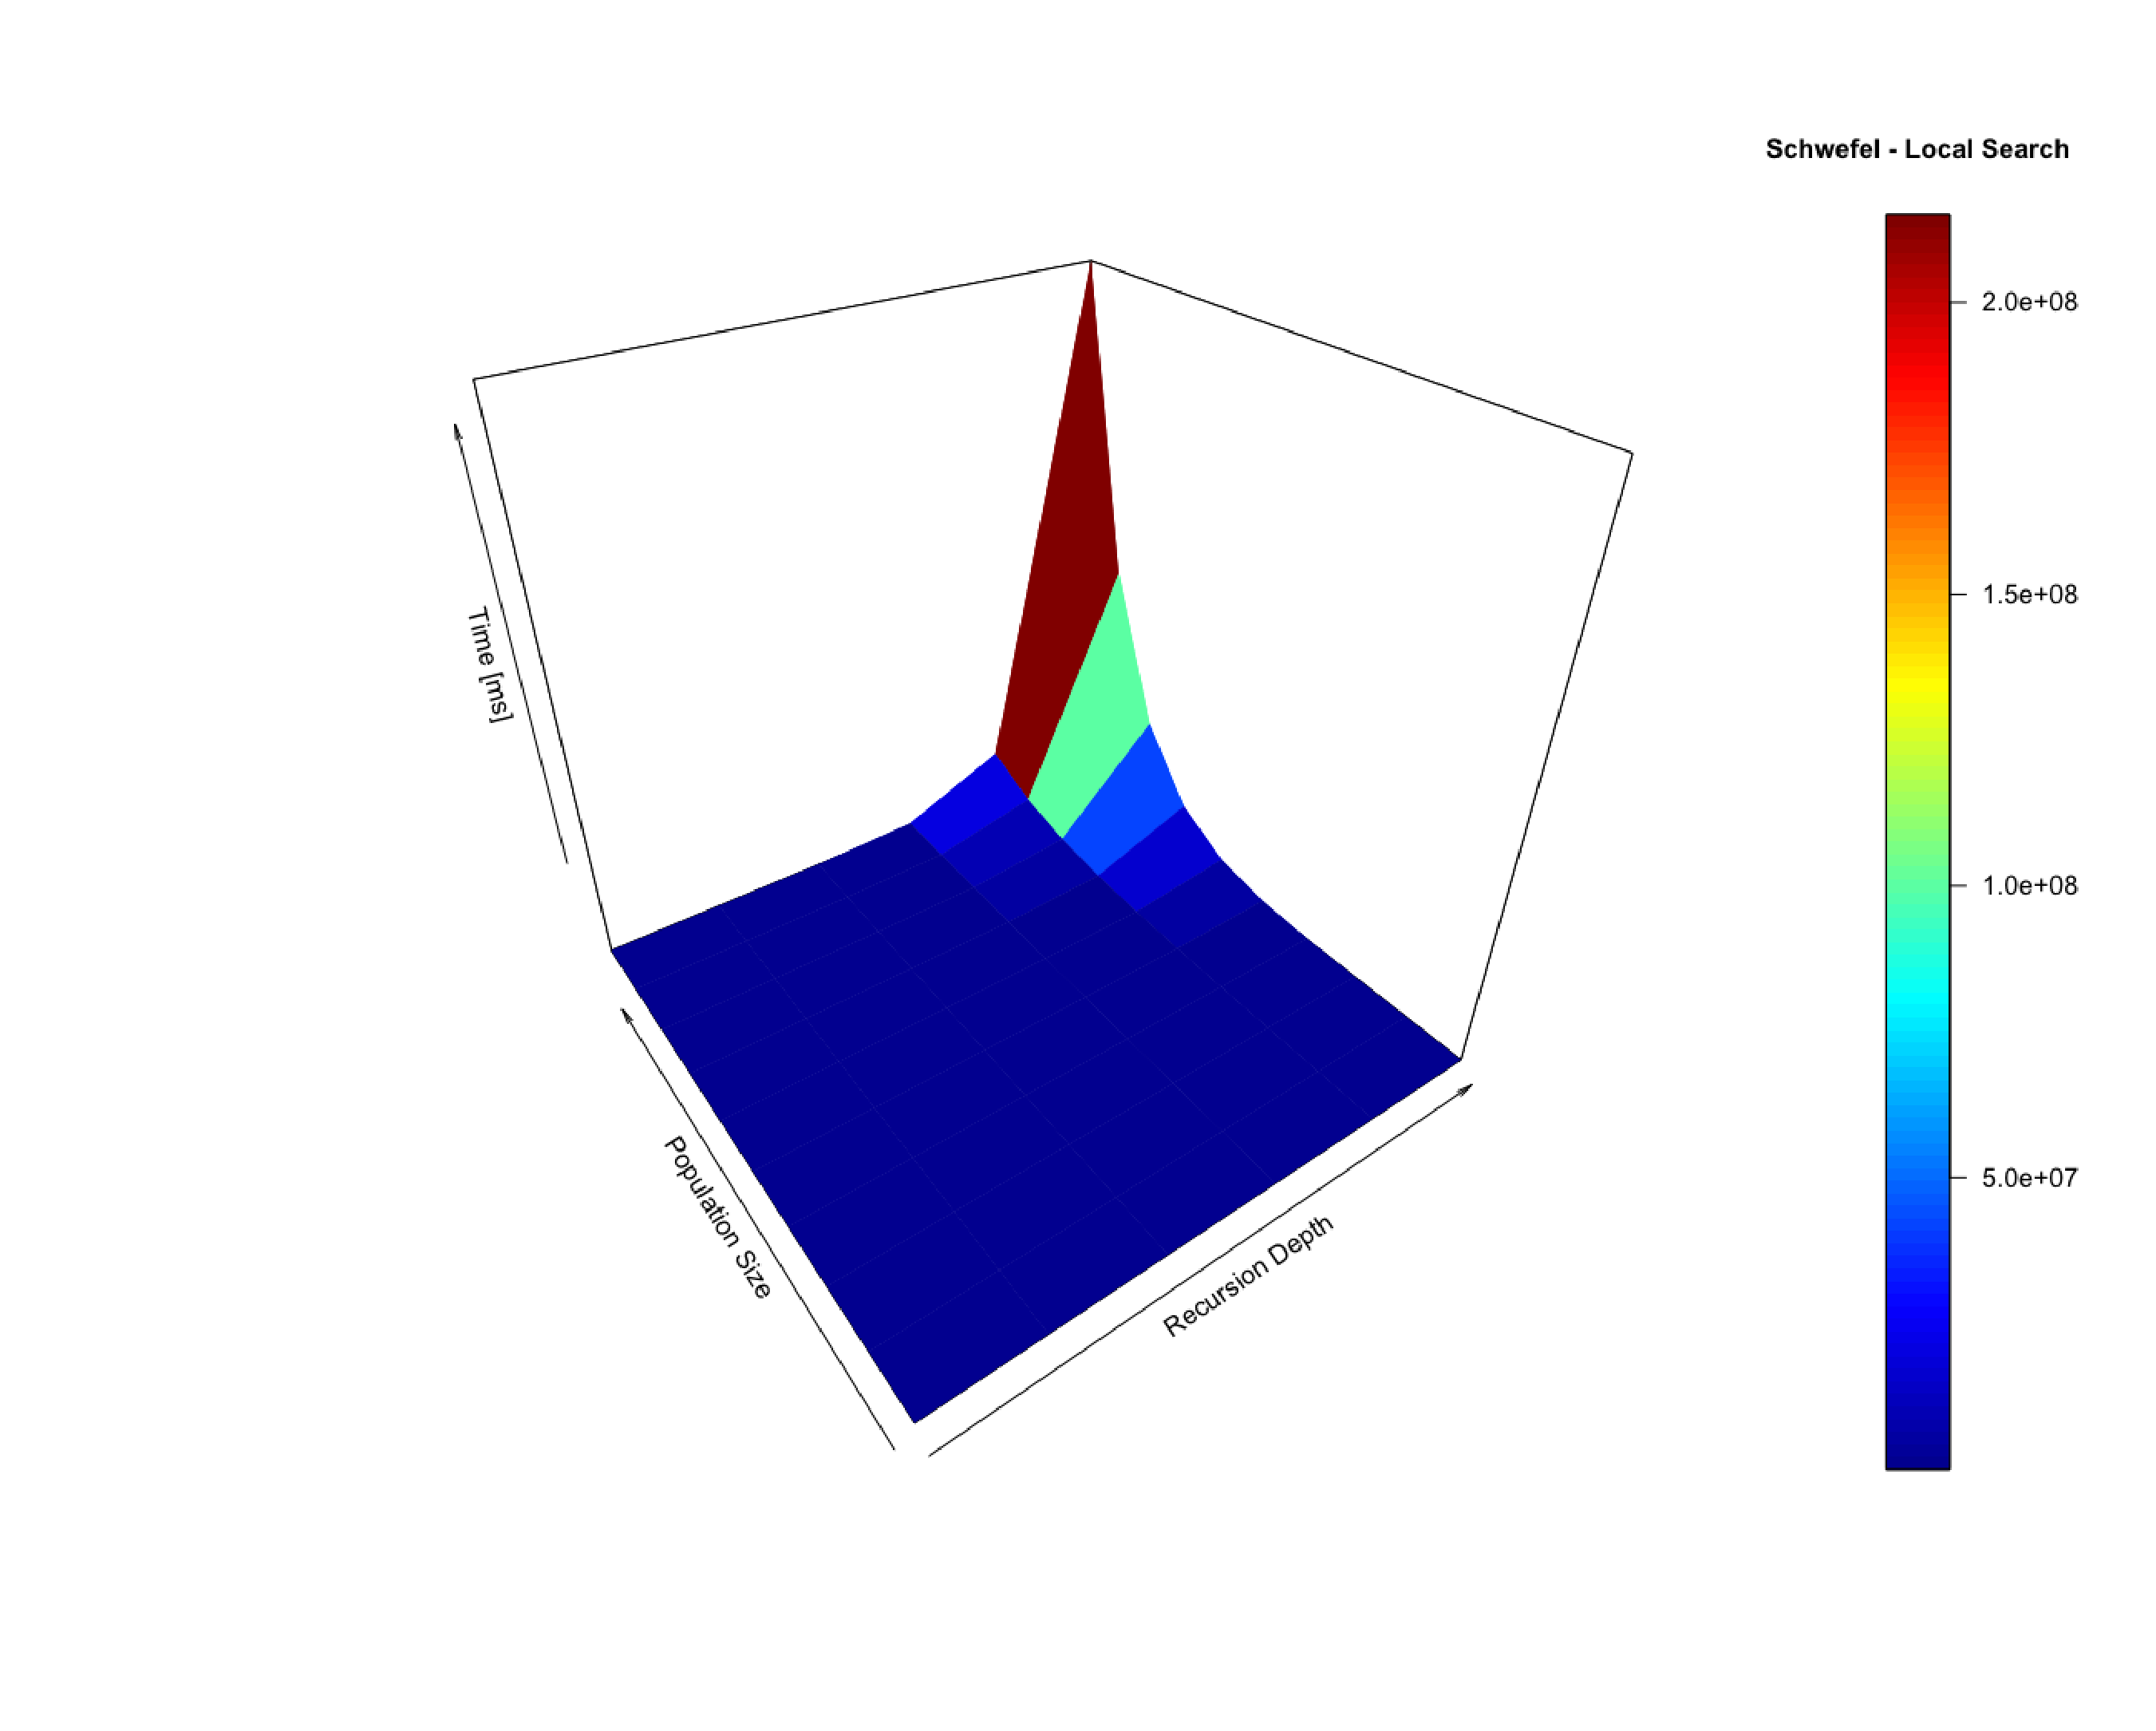
\includegraphics[width=1.0\hsize,height=0.65\hsize]{fig08.eps}
\caption{Schwefel - Local Search - Time[ms]}
\label{fig13}
\end{figure}

\begin{figure}[tbp]
\centering
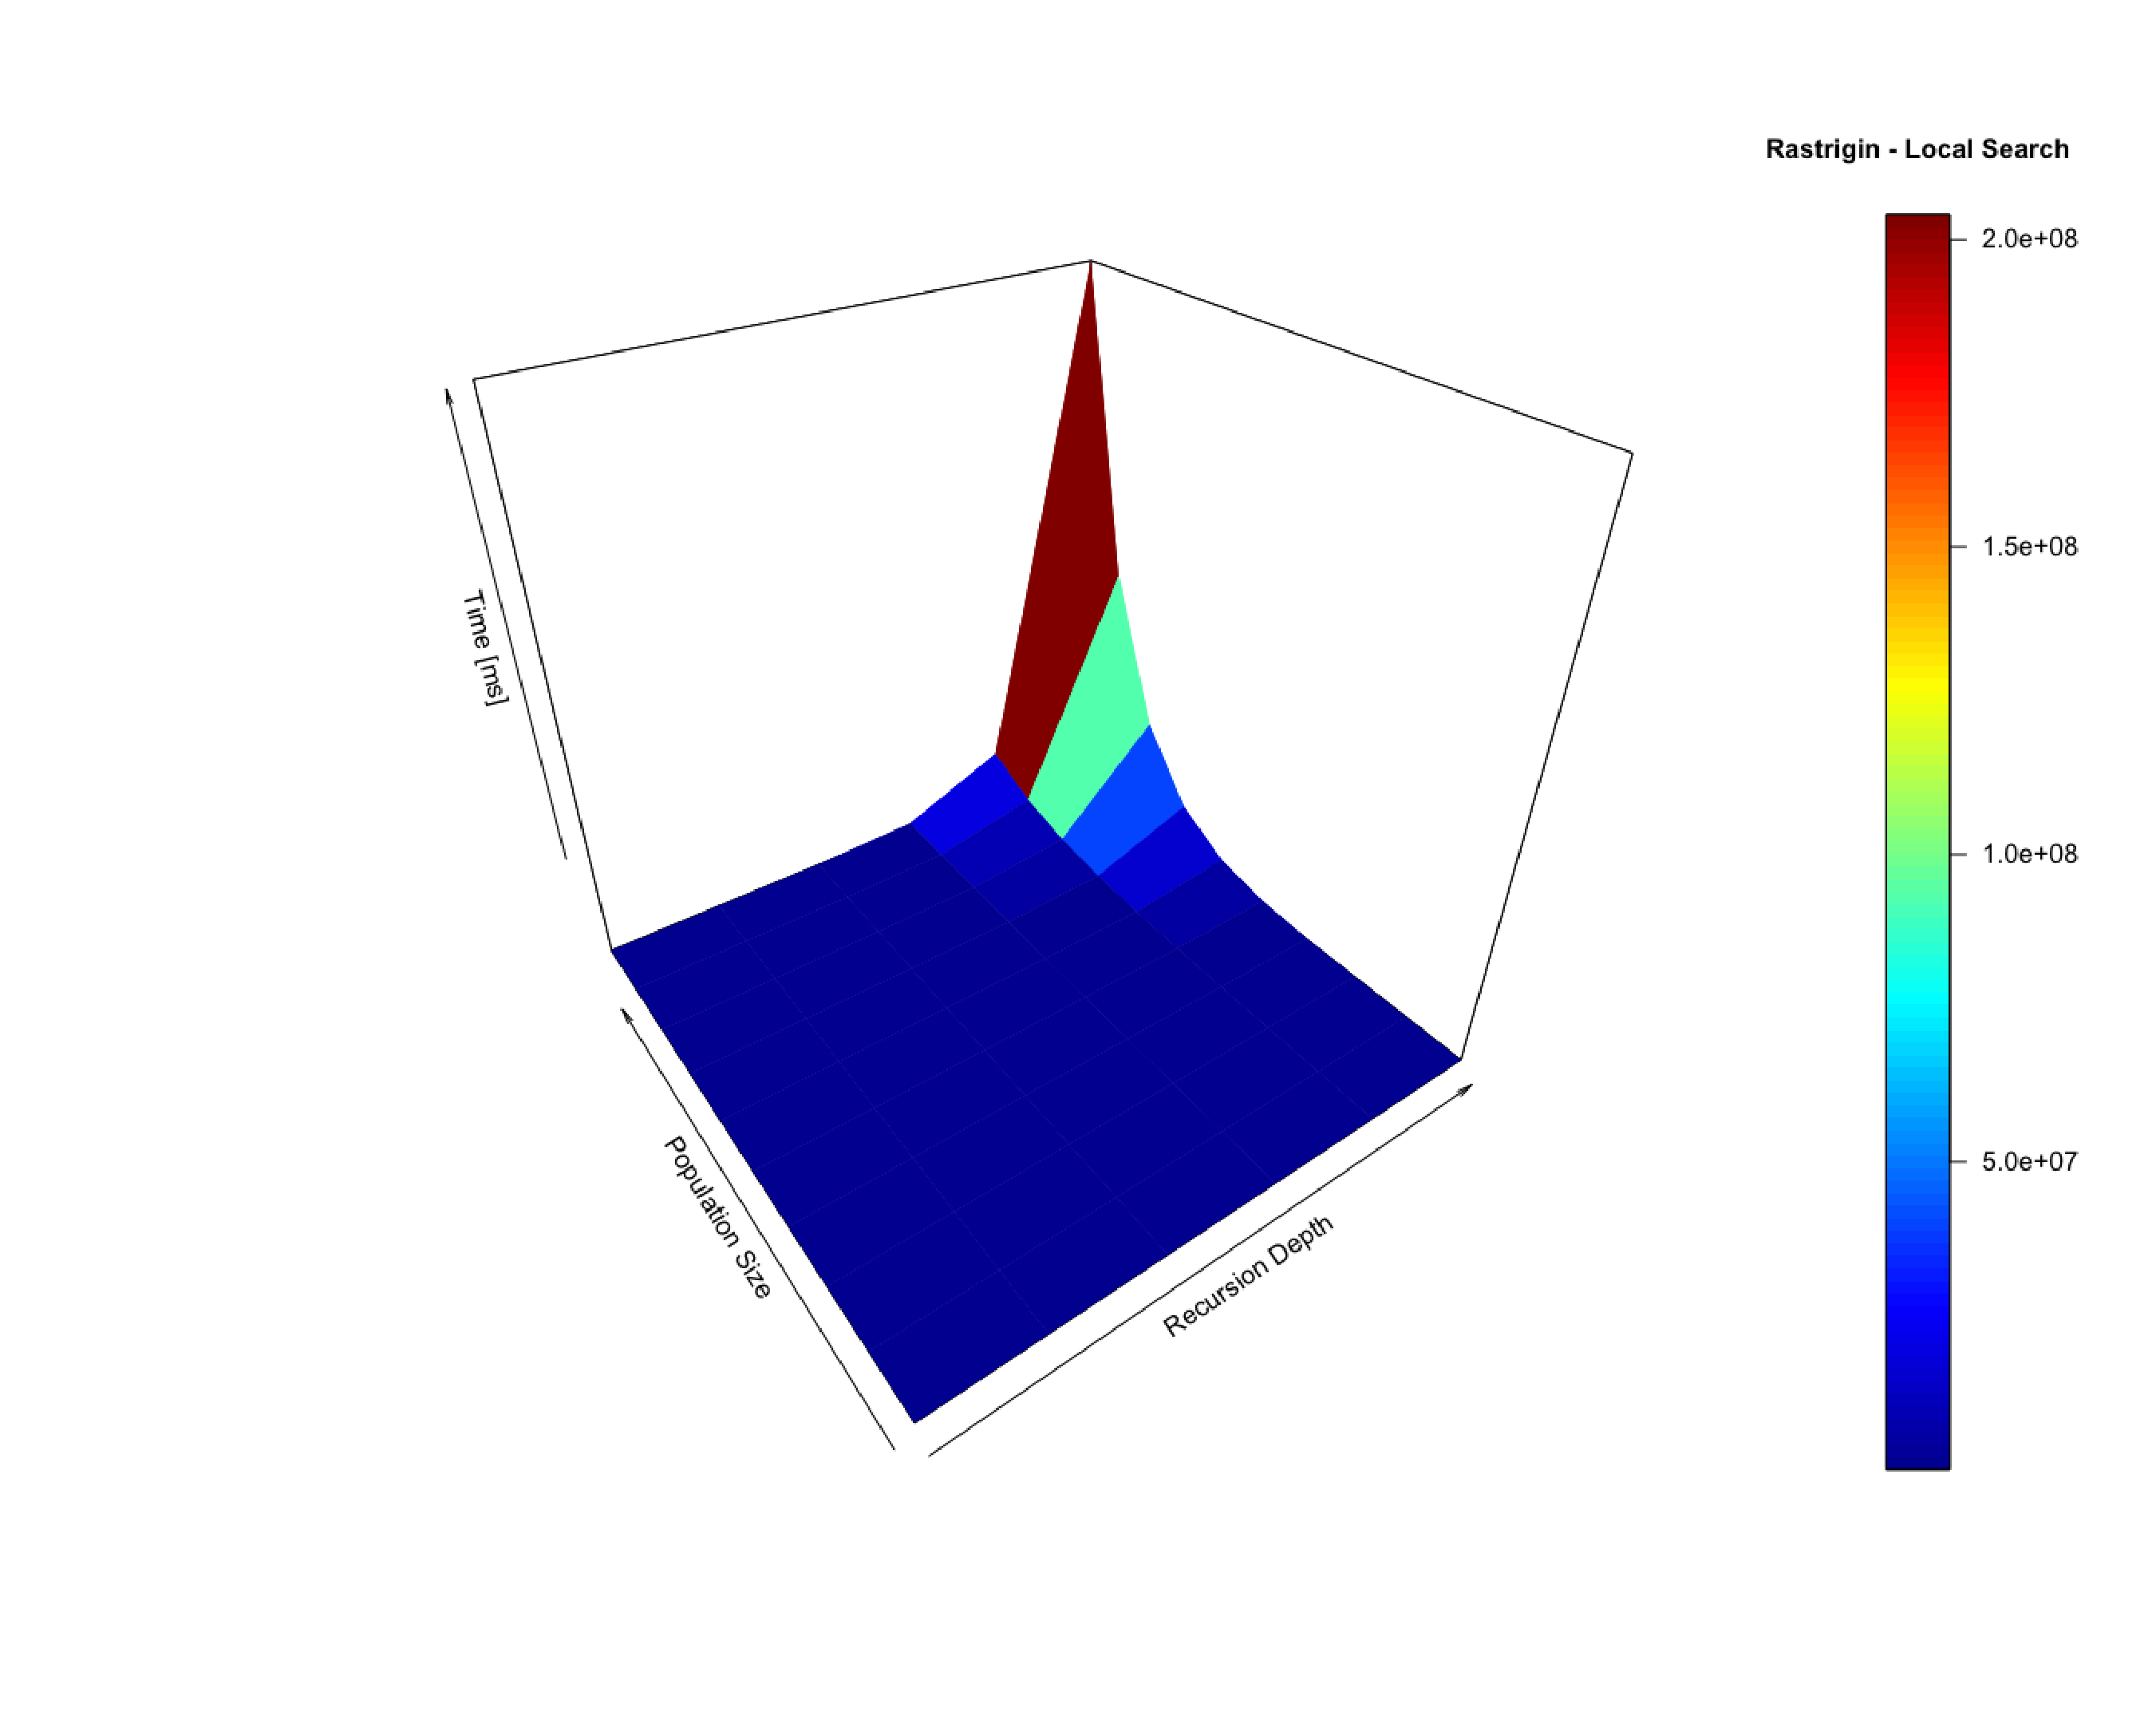
\includegraphics[width=1.0\hsize,height=0.65\hsize]{fig11.eps}
\caption{Rastrigin - Local Search - Time[ms]}
\label{fig14}
\end{figure}

\begin{figure}[tbp]
\centering
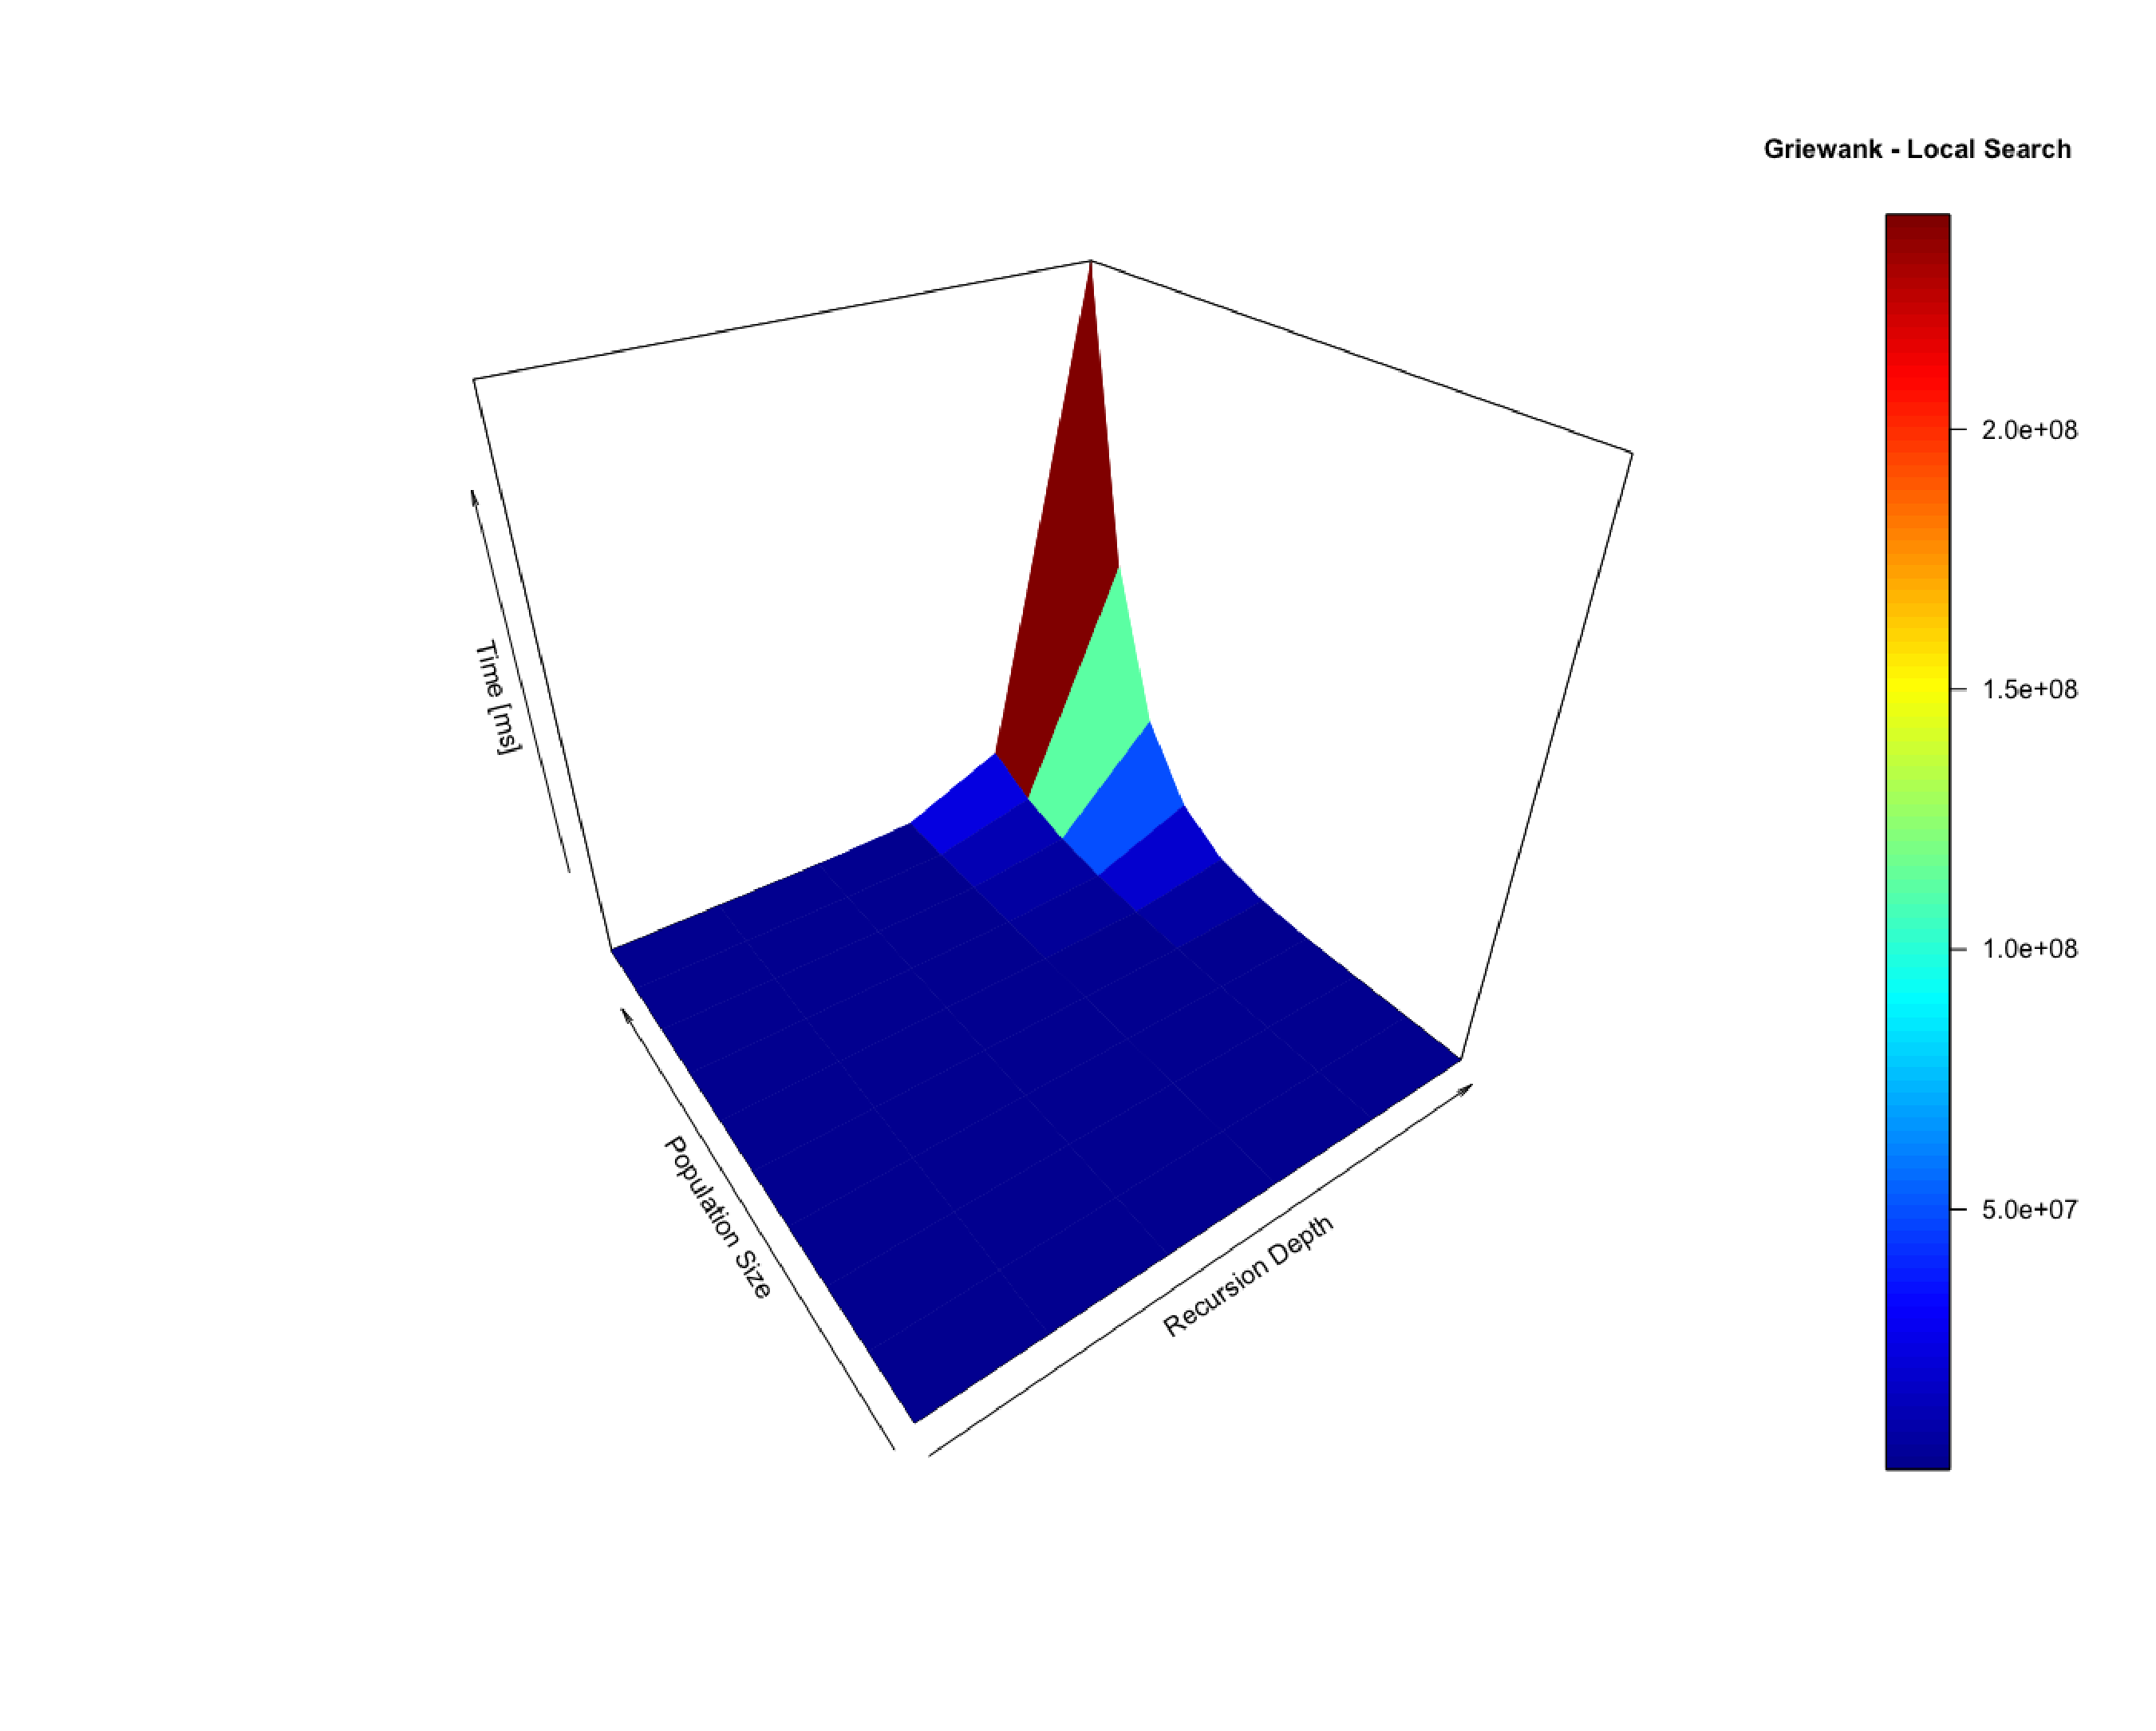
\includegraphics[width=1.0\hsize,height=0.65\hsize]{fig14.eps}
\caption{Griewank - Local Search - Time[ms]}
\label{fig15}
\end{figure}

\begin{figure}[tbp]
\centering
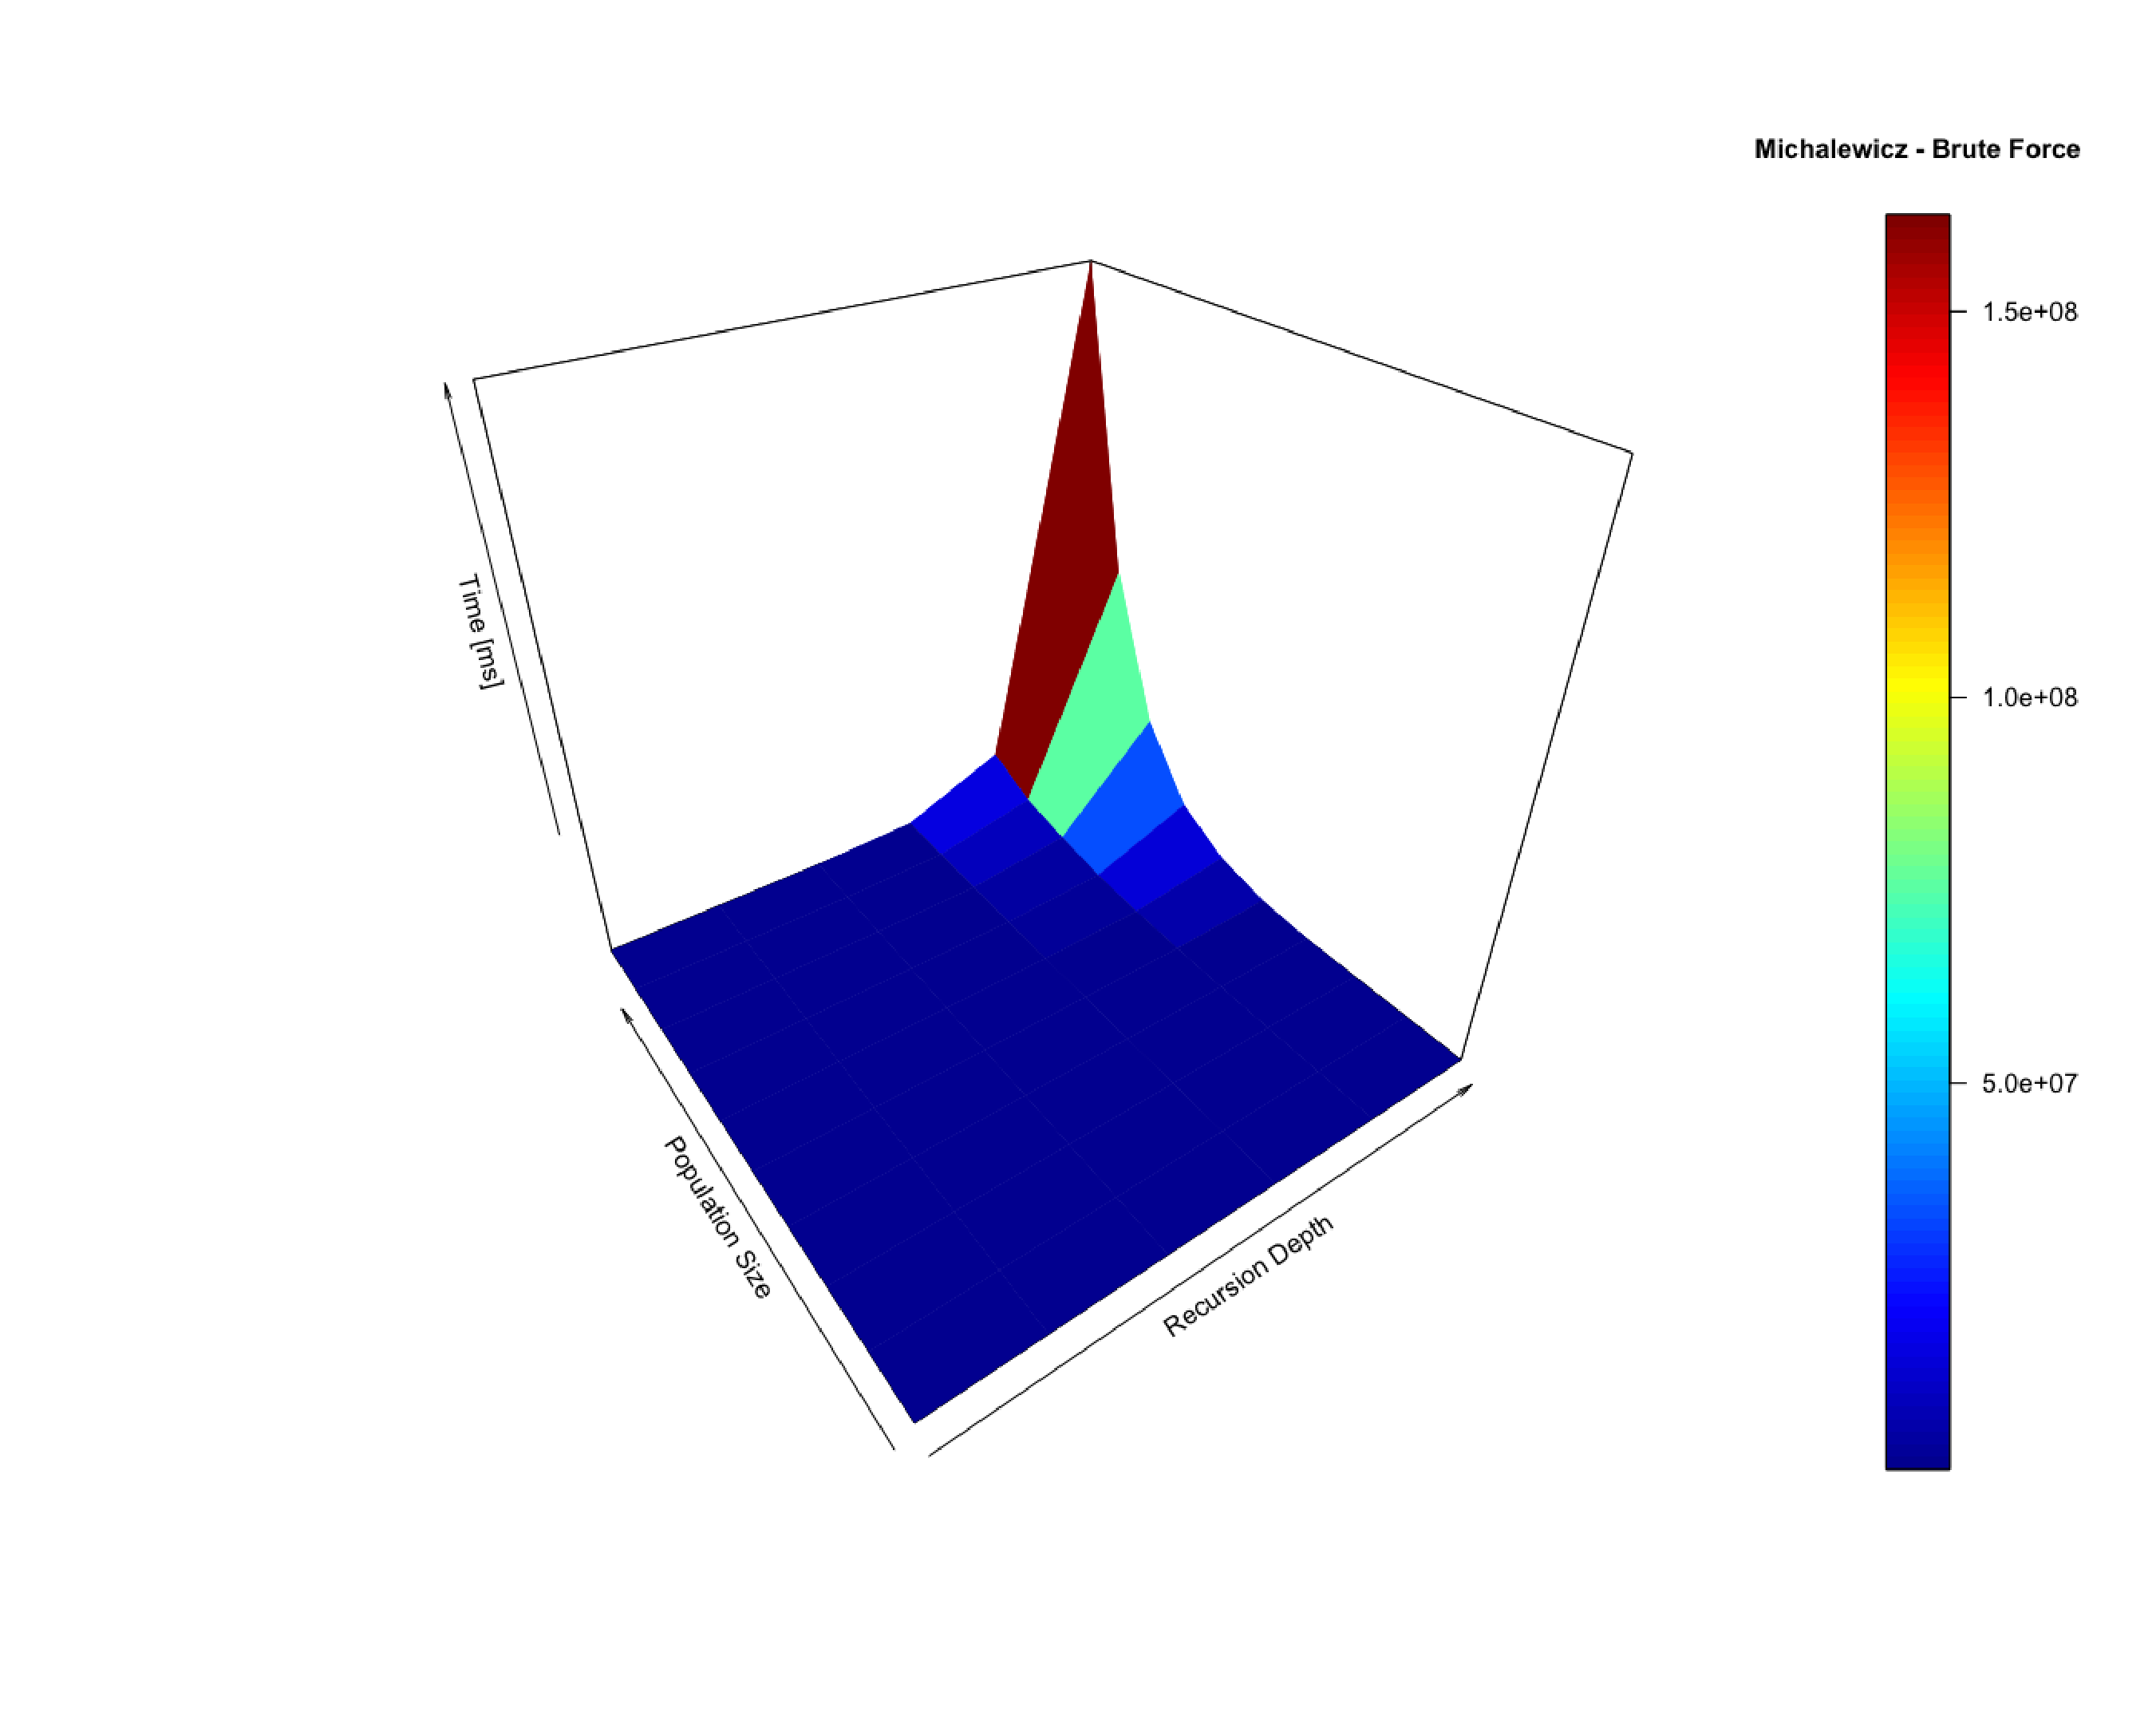
\includegraphics[width=1.0\hsize,height=0.65\hsize]{fig17.eps}
\caption{Michalewicz - Brute Force - Time[ms]}
\label{fig16}
\end{figure}

\begin{figure}[tbp]
\centering
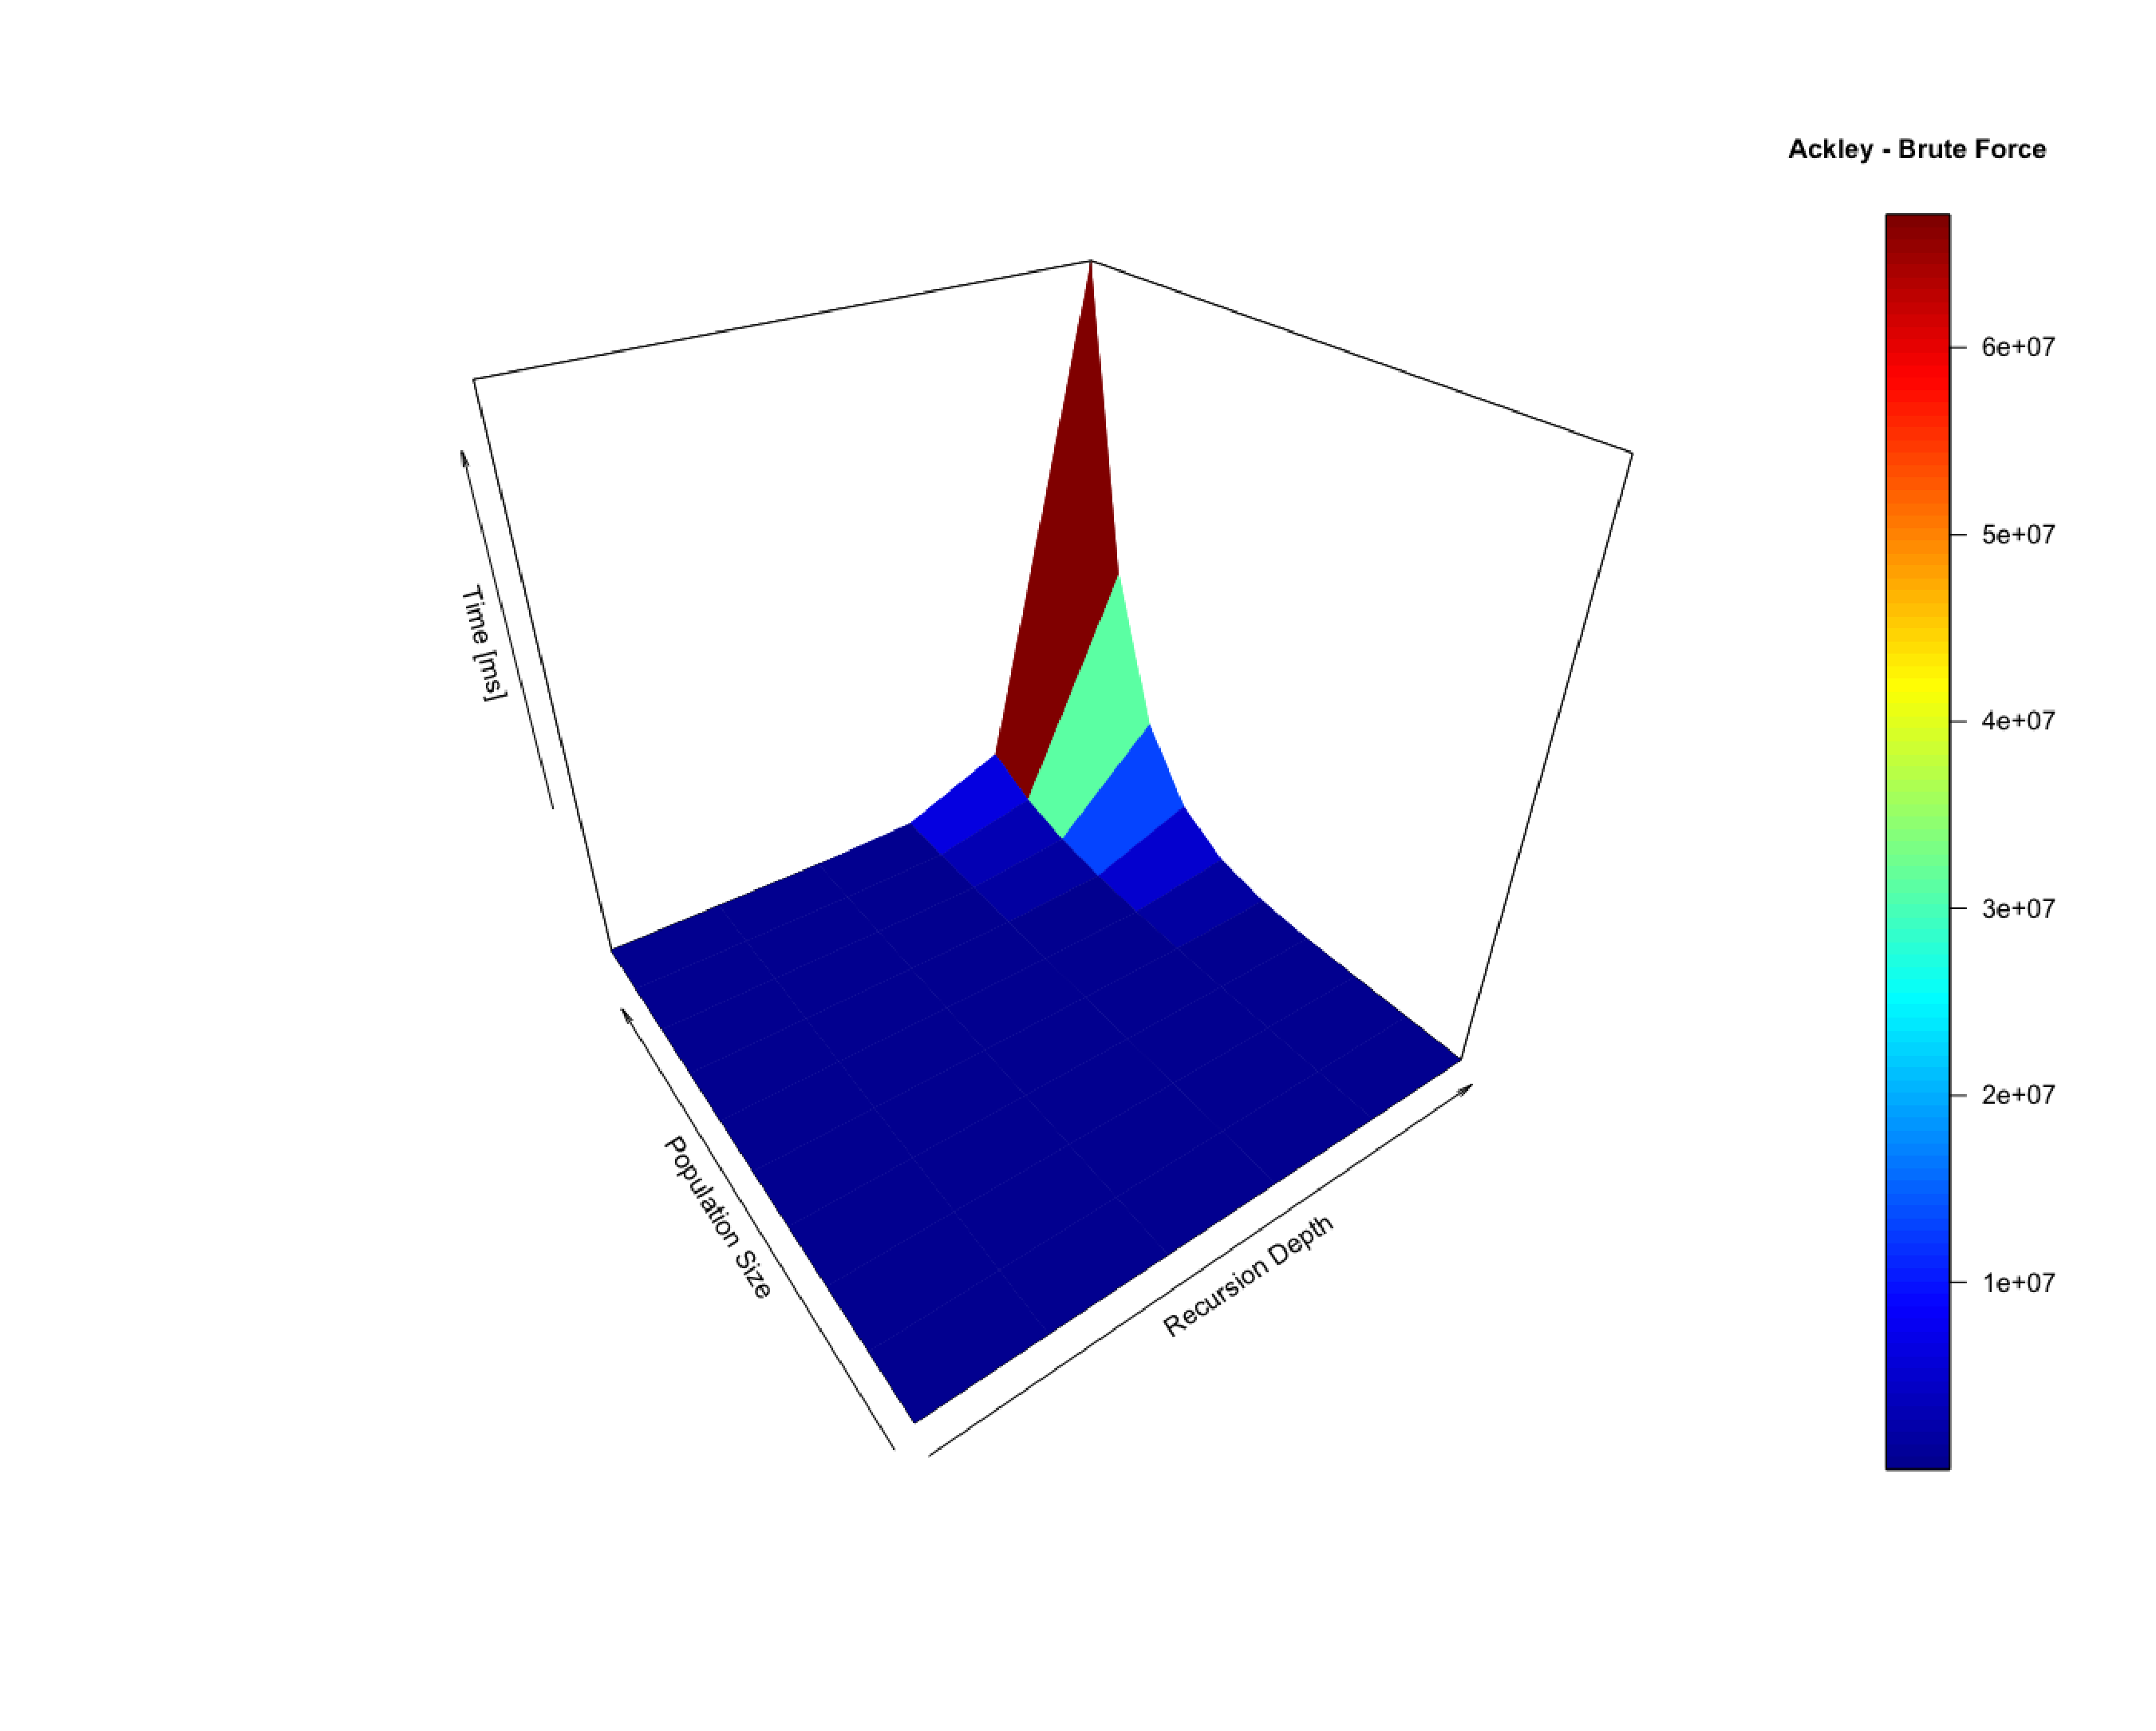
\includegraphics[width=1.0\hsize,height=0.65\hsize]{fig20.eps}
\caption{Ackley - Brute Force - Time[ms]}
\label{fig17}
\end{figure}

\begin{figure}[tbp]
\centering
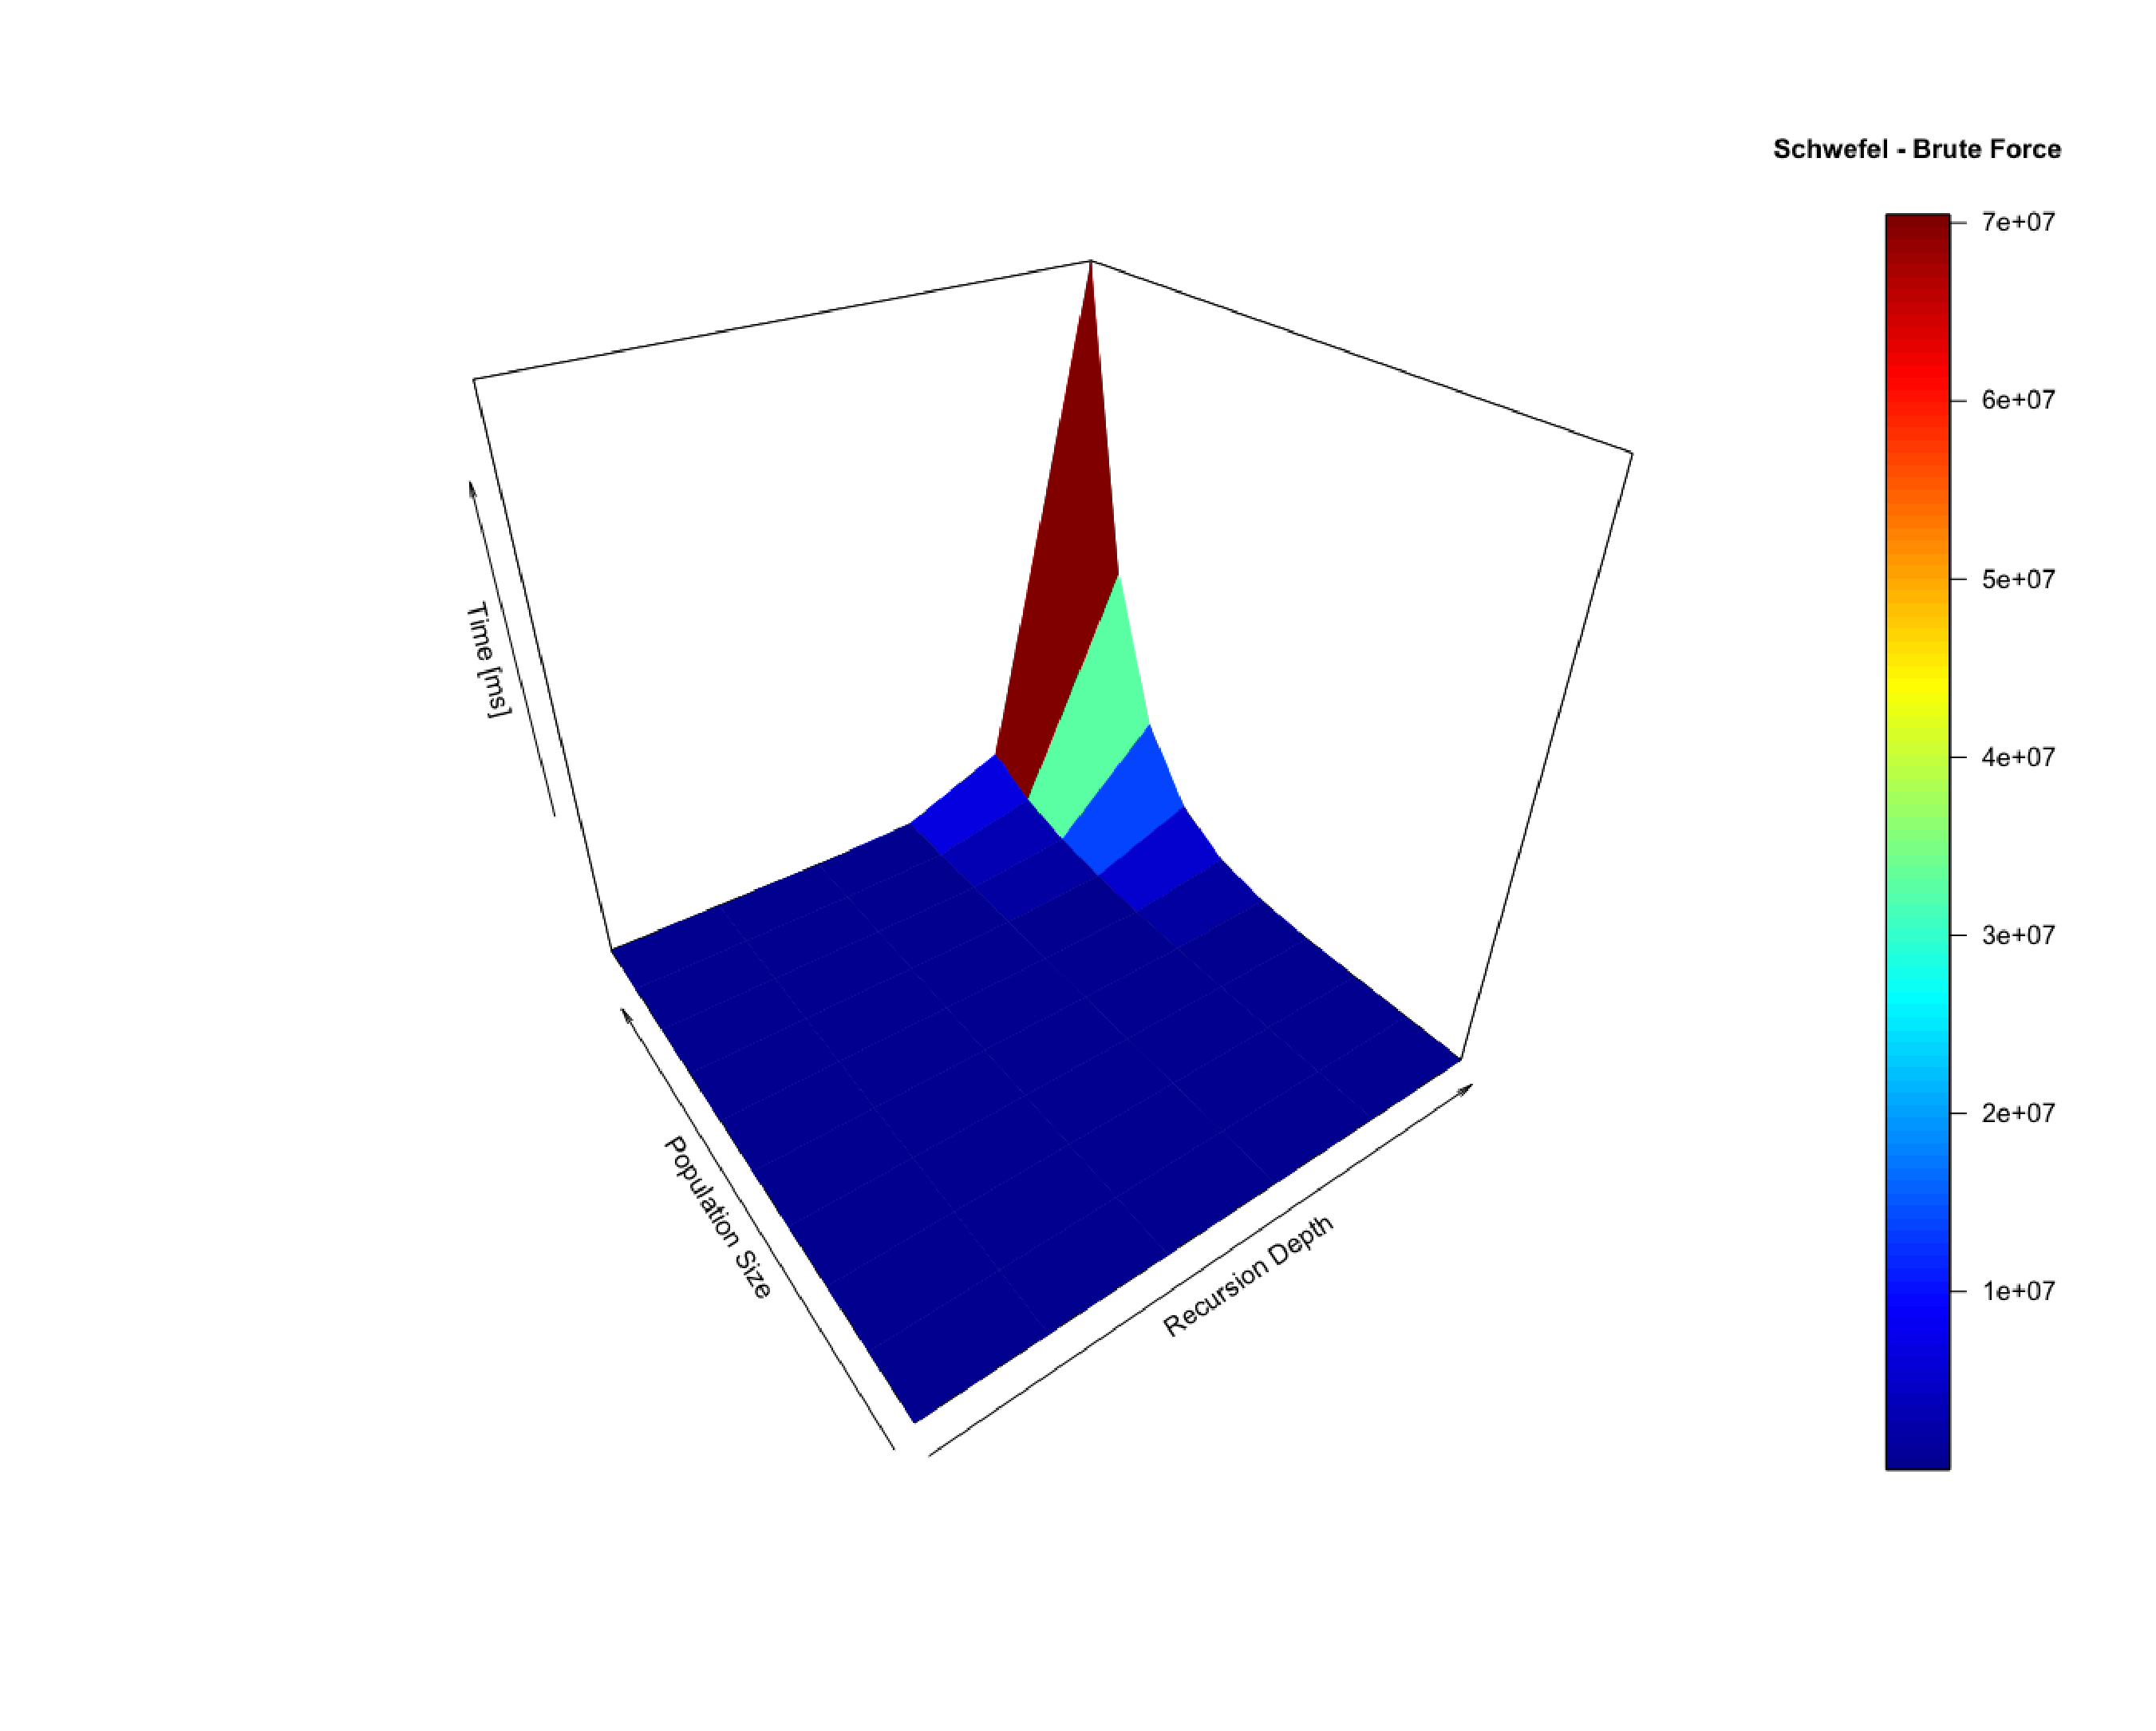
\includegraphics[width=1.0\hsize,height=0.65\hsize]{fig23.eps}
\caption{Schwefel - Brute Force - Time[ms]}
\label{fig18}
\end{figure}

\begin{figure}[tbp]
\centering
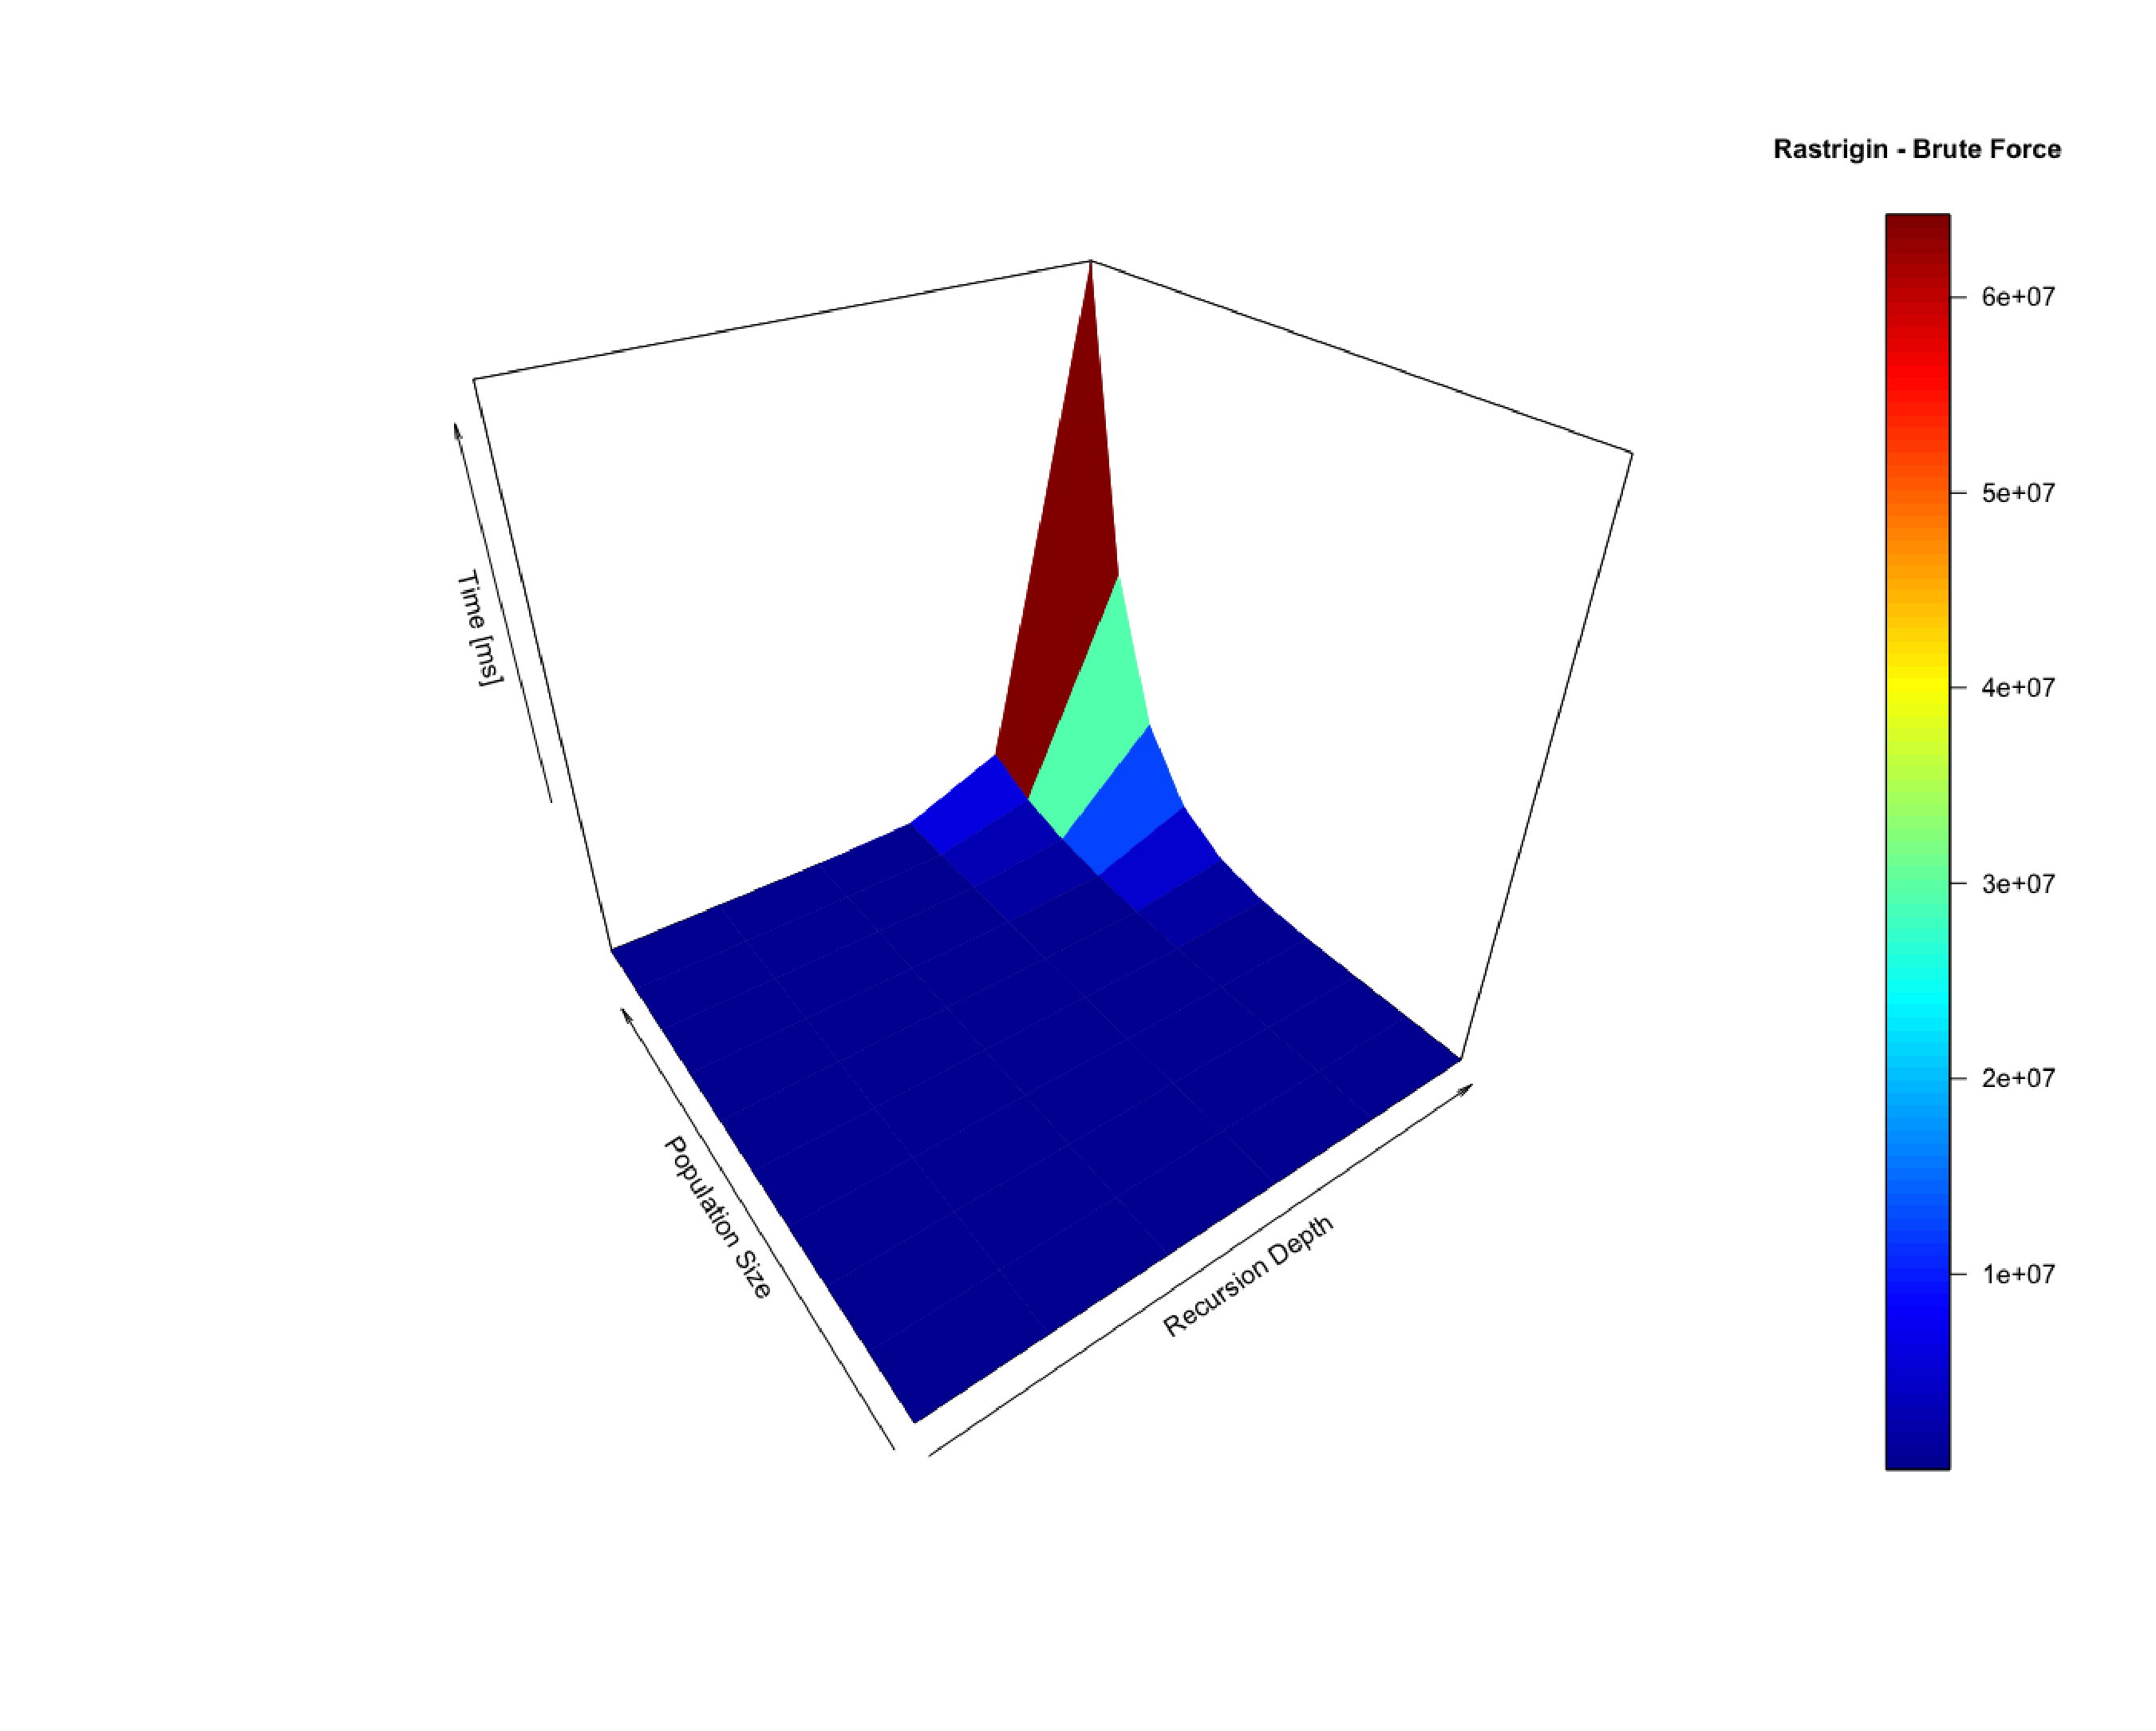
\includegraphics[width=1.0\hsize,height=0.65\hsize]{fig26.eps}
\caption{Rastrigin - Brute Force - Time[ms]}
\label{fig19}
\end{figure}

\begin{figure}[tbp]
\centering
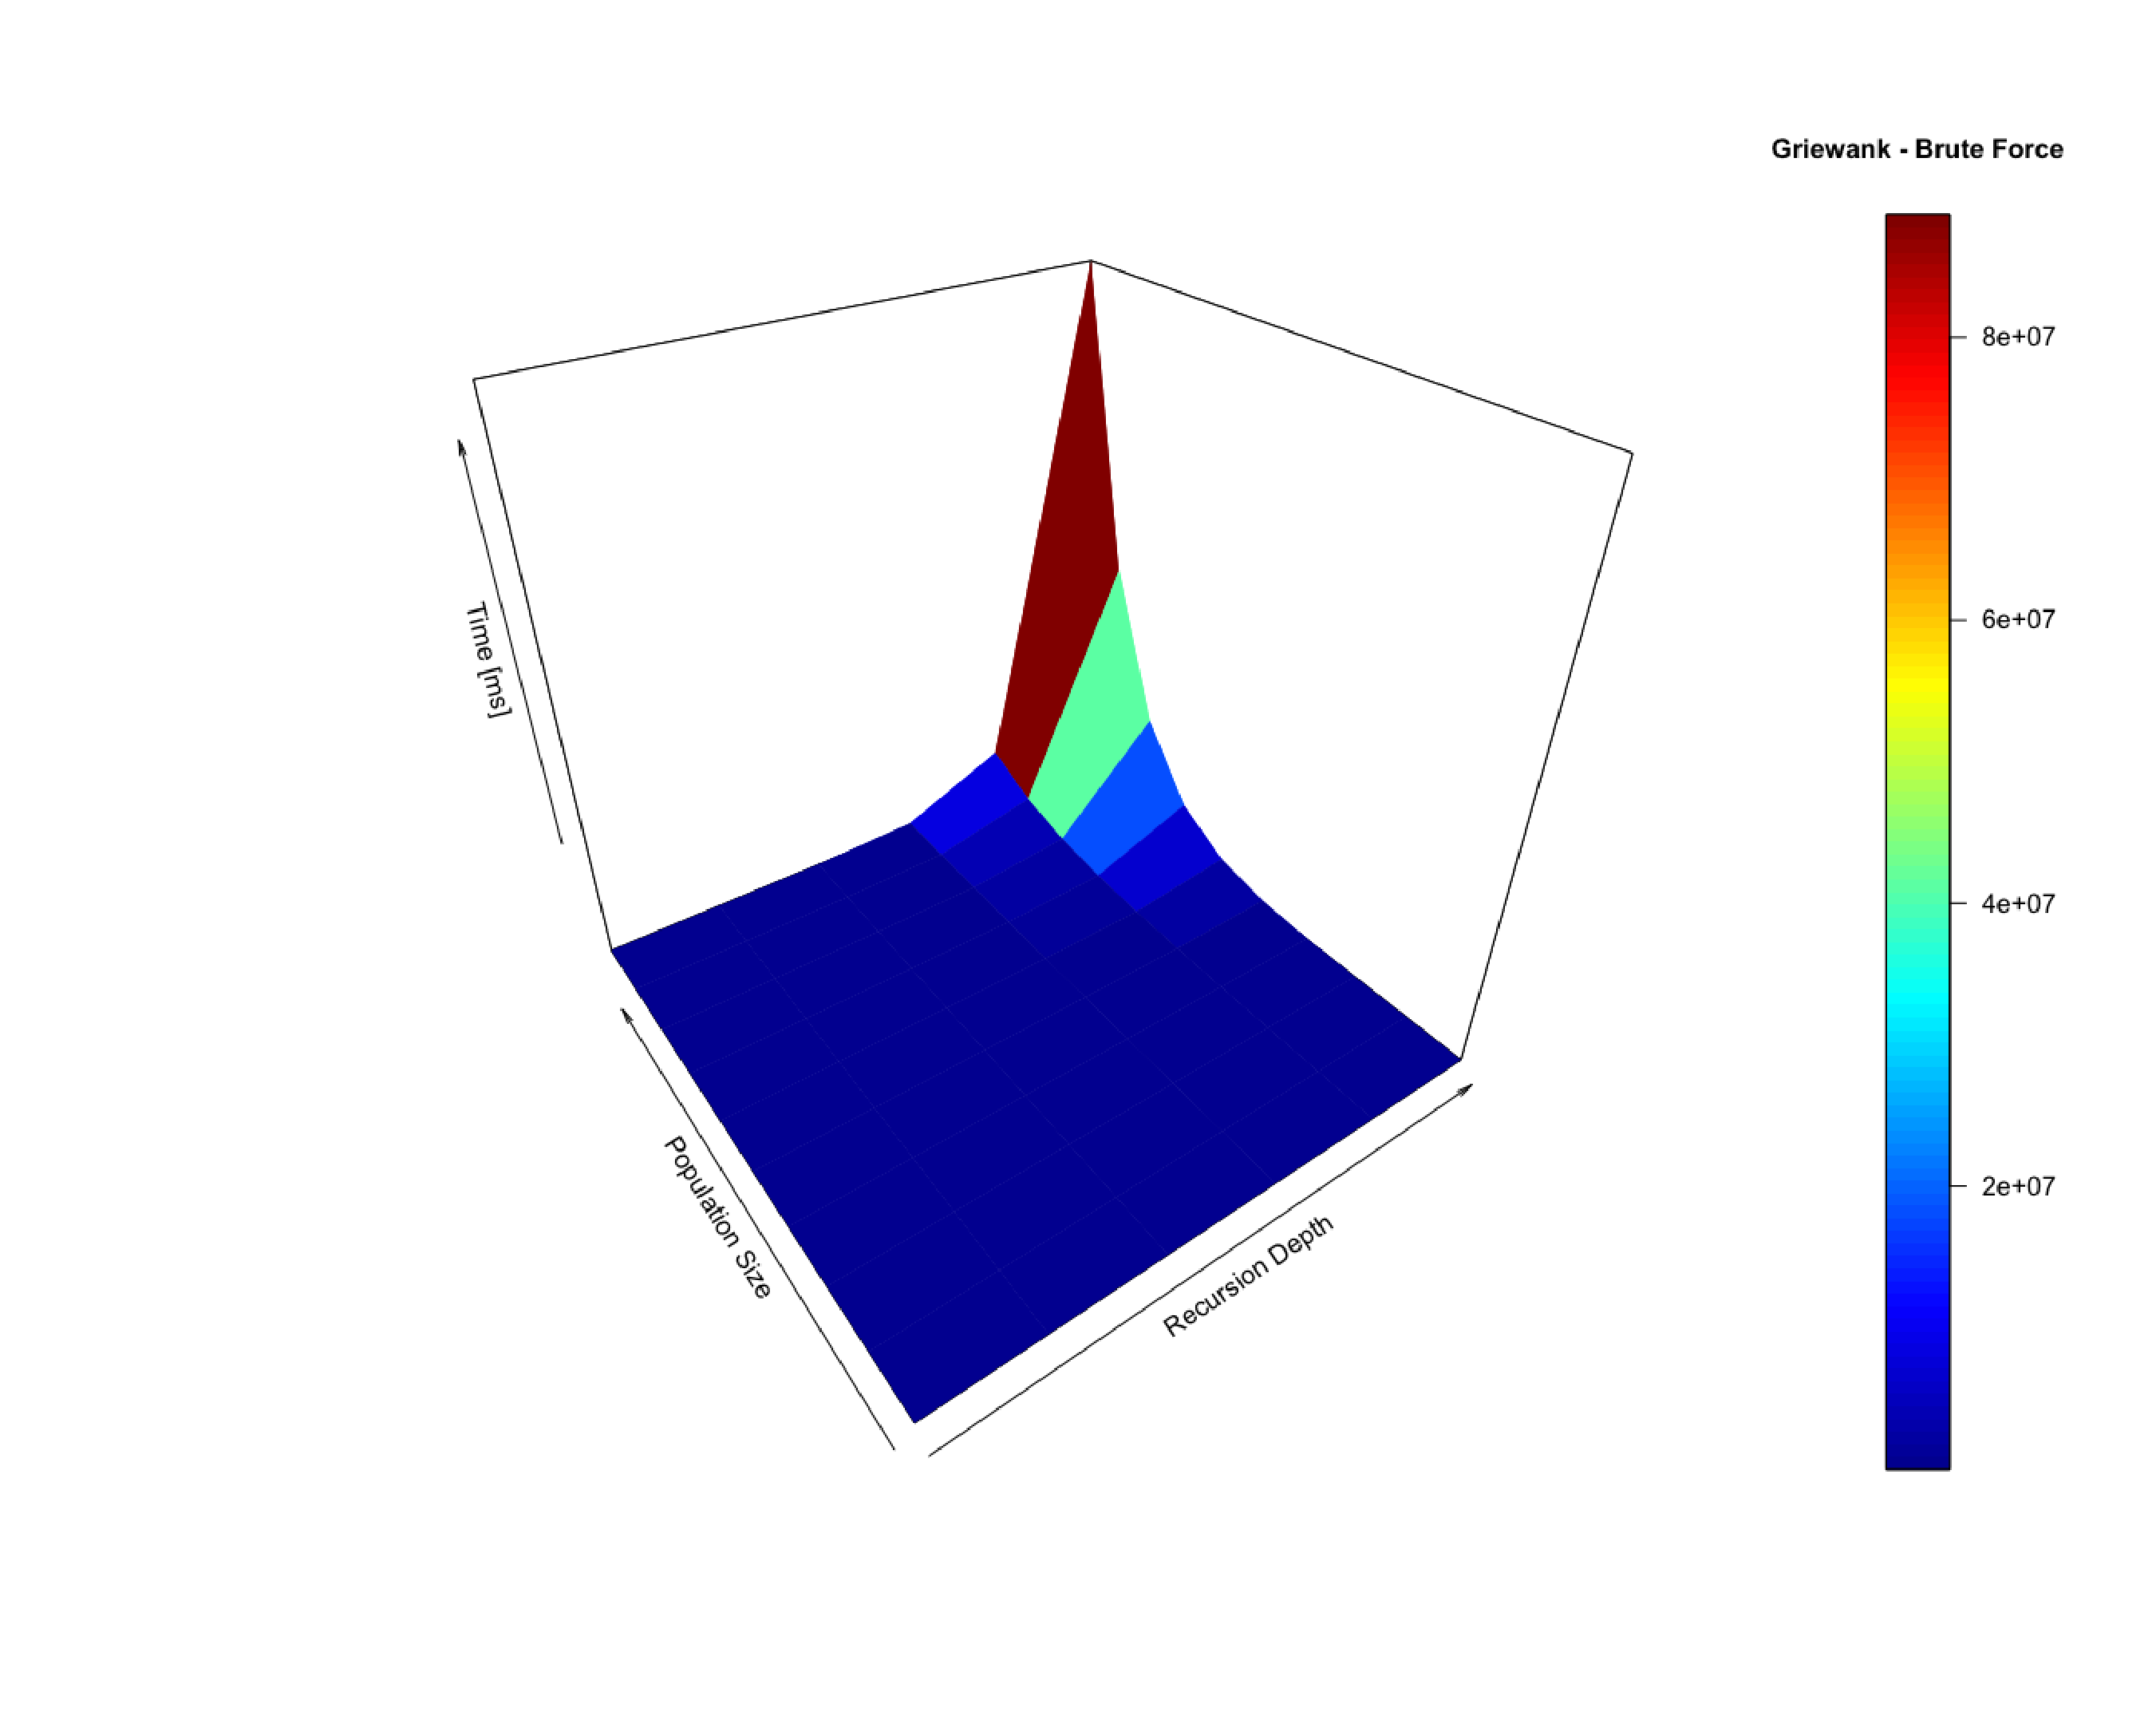
\includegraphics[width=1.0\hsize,height=0.65\hsize]{fig29.eps}
\caption{Griewank - Brute Force - Time[ms]}
\label{fig20}
\end{figure}

\begin{figure}[tbp]
\centering
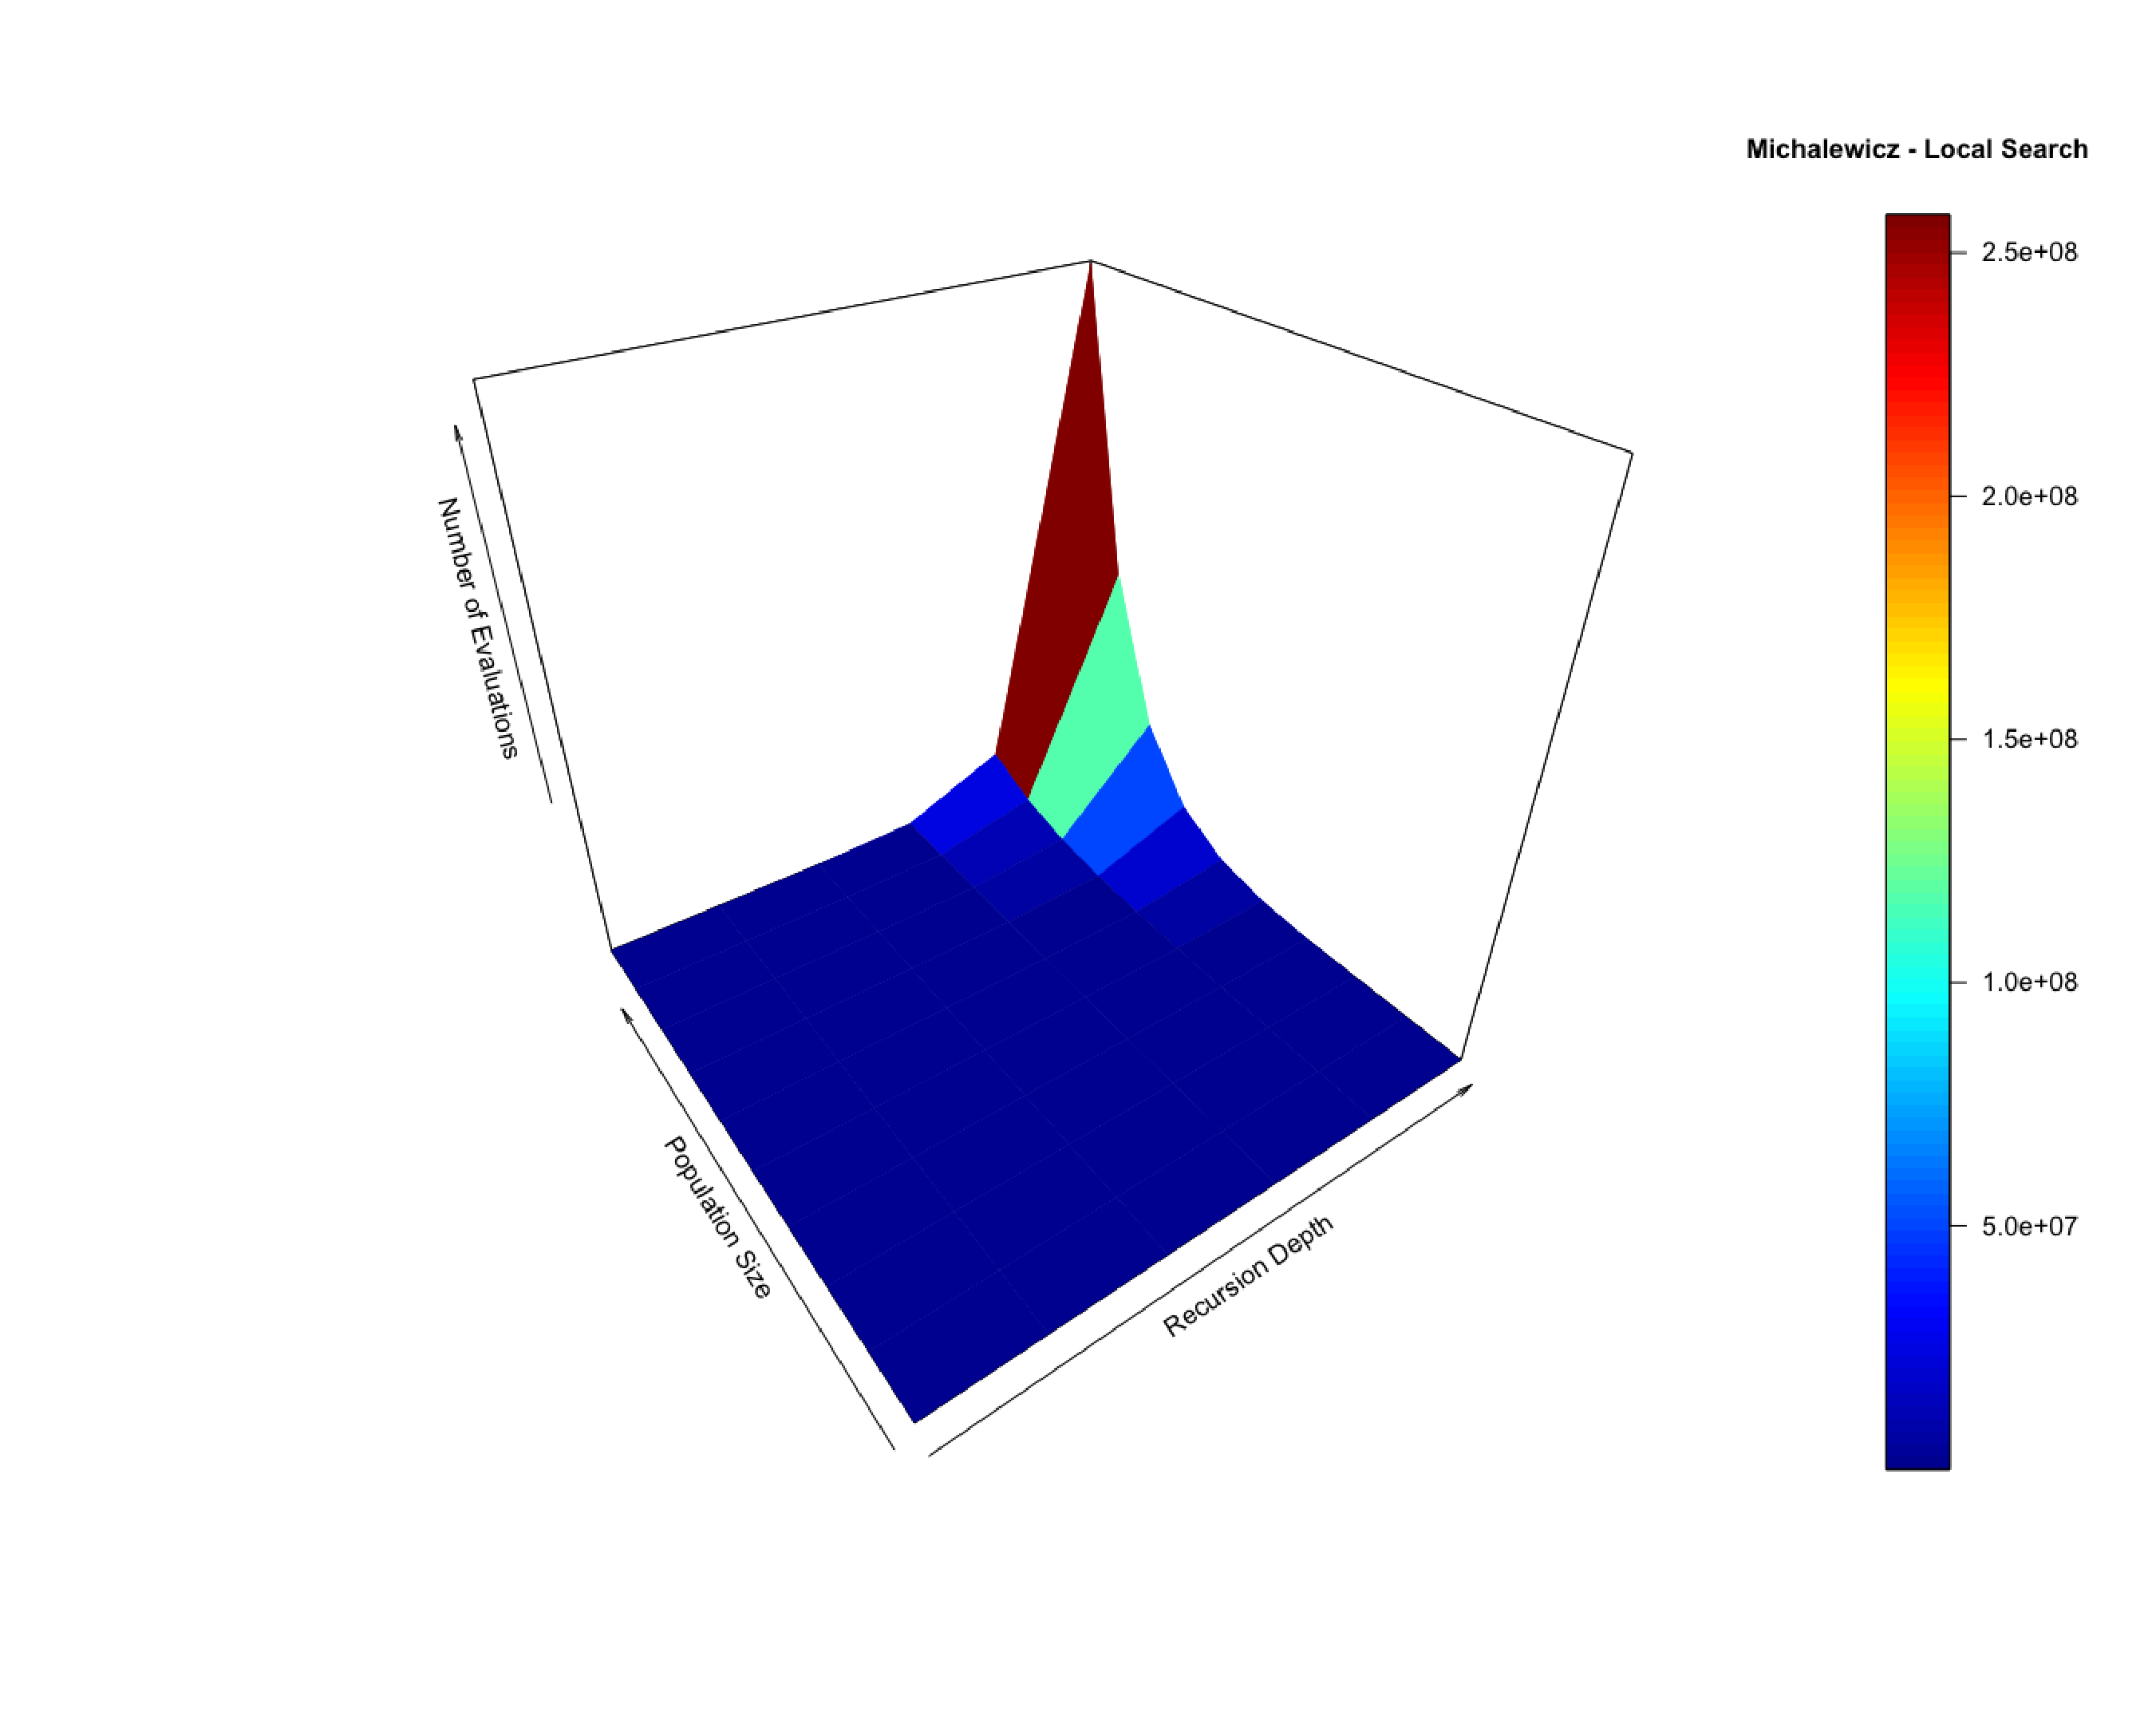
\includegraphics[width=1.0\hsize,height=0.65\hsize]{fig04.eps}
\caption{Michalewicz - Local Search - Fitness Evaluations}
\label{fig21}
\end{figure}

\begin{figure}[tbp]
\centering
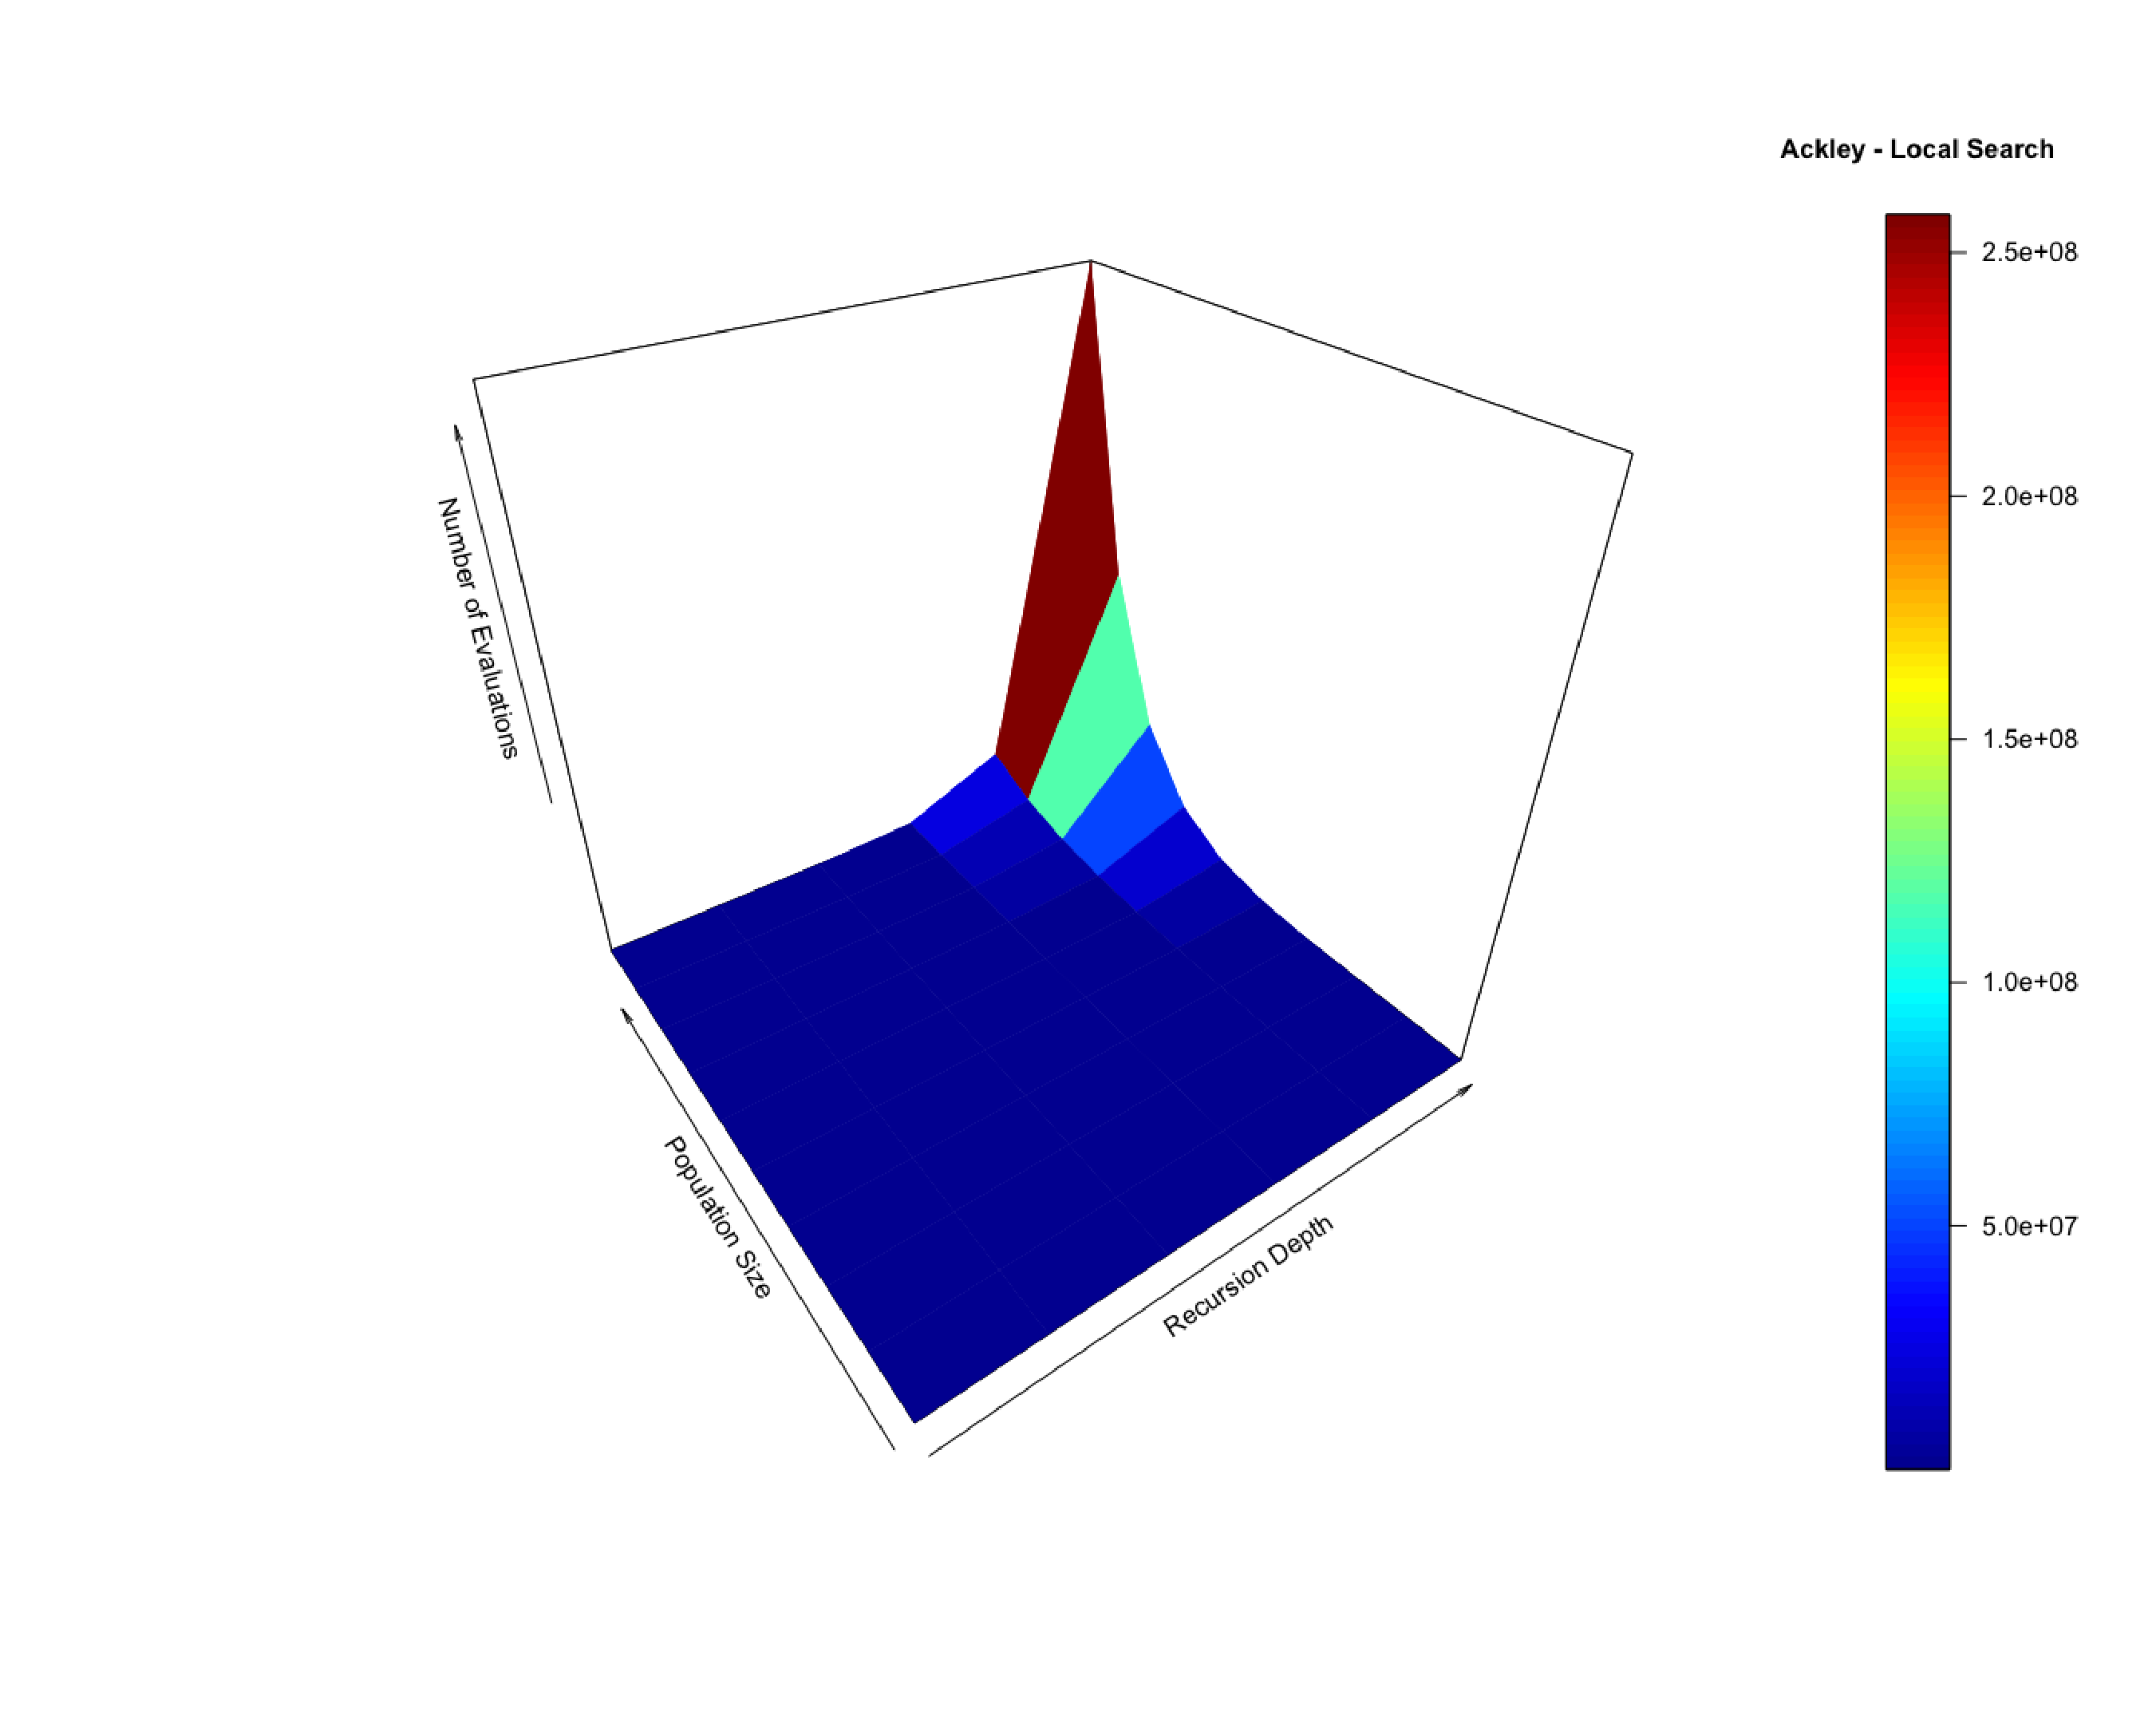
\includegraphics[width=1.0\hsize,height=0.65\hsize]{fig07.eps}
\caption{Ackley - Local Search - Fitness Evaluations}
\label{fig22}
\end{figure}

\begin{figure}[tbp]
\centering
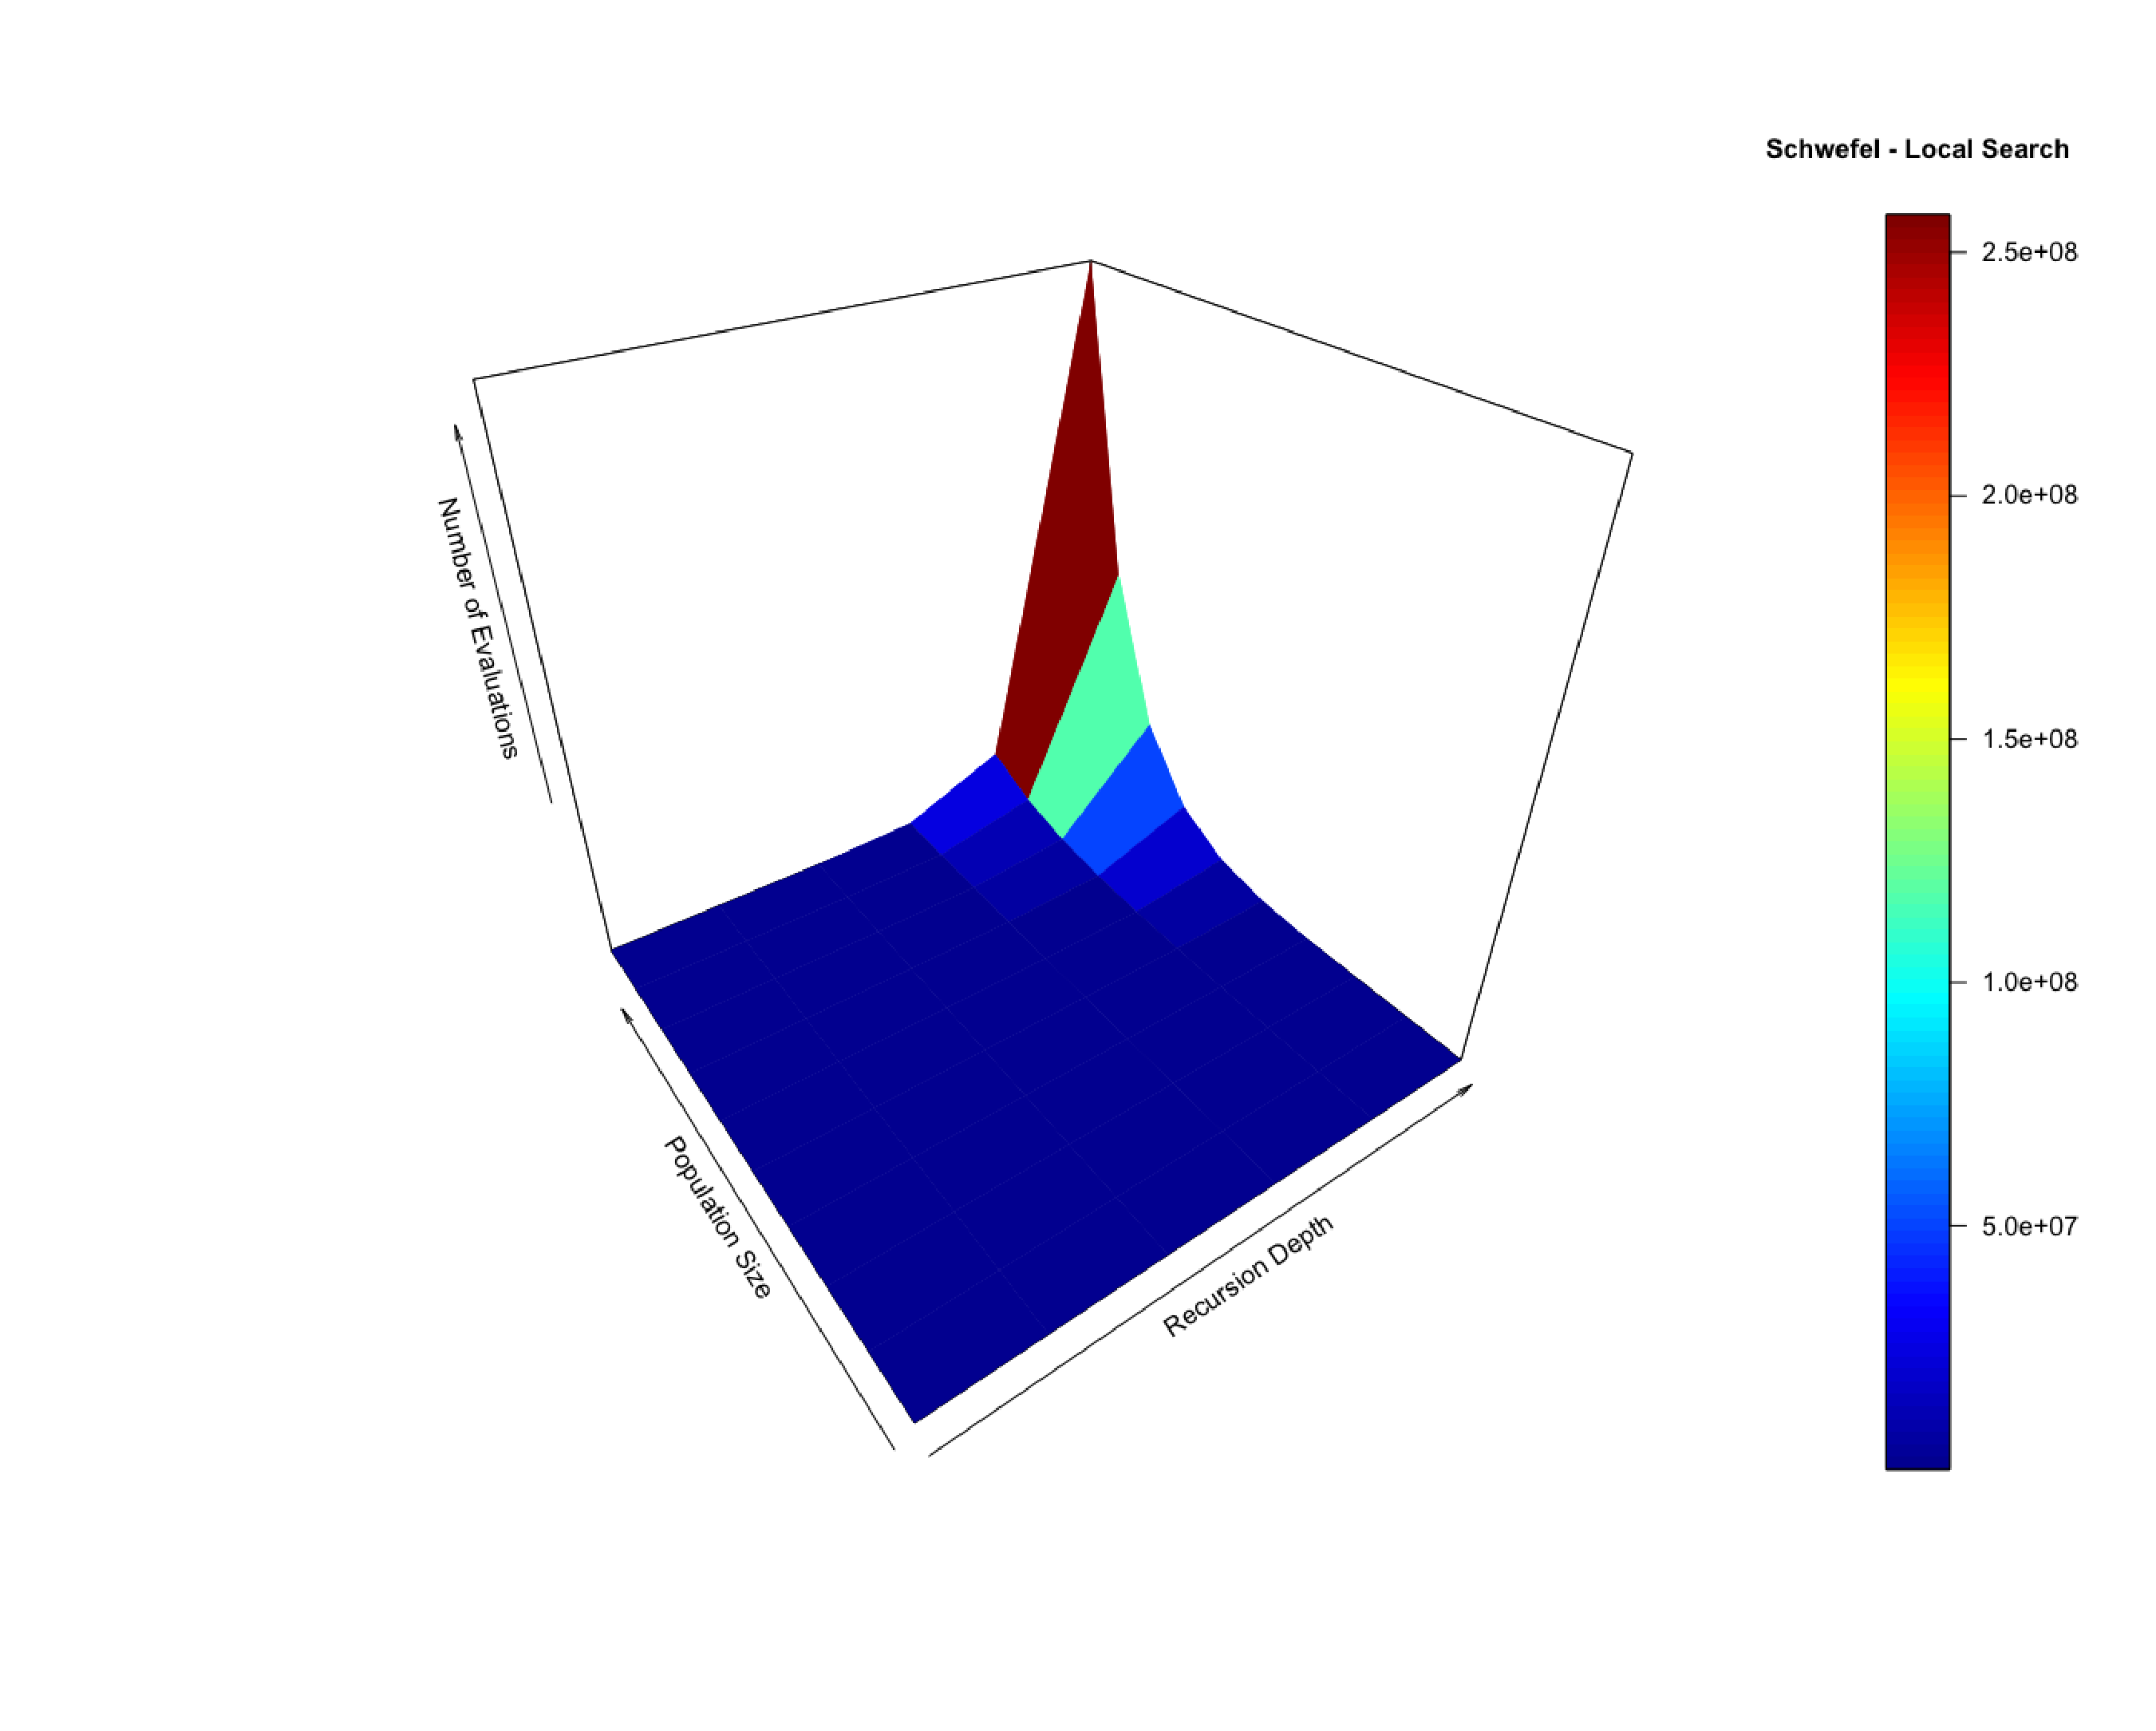
\includegraphics[width=1.0\hsize,height=0.65\hsize]{fig10.eps}
\caption{Schwefel - Local Search - Fitness Evaluations}
\label{fig23}
\end{figure}

\begin{figure}[tbp]
\centering
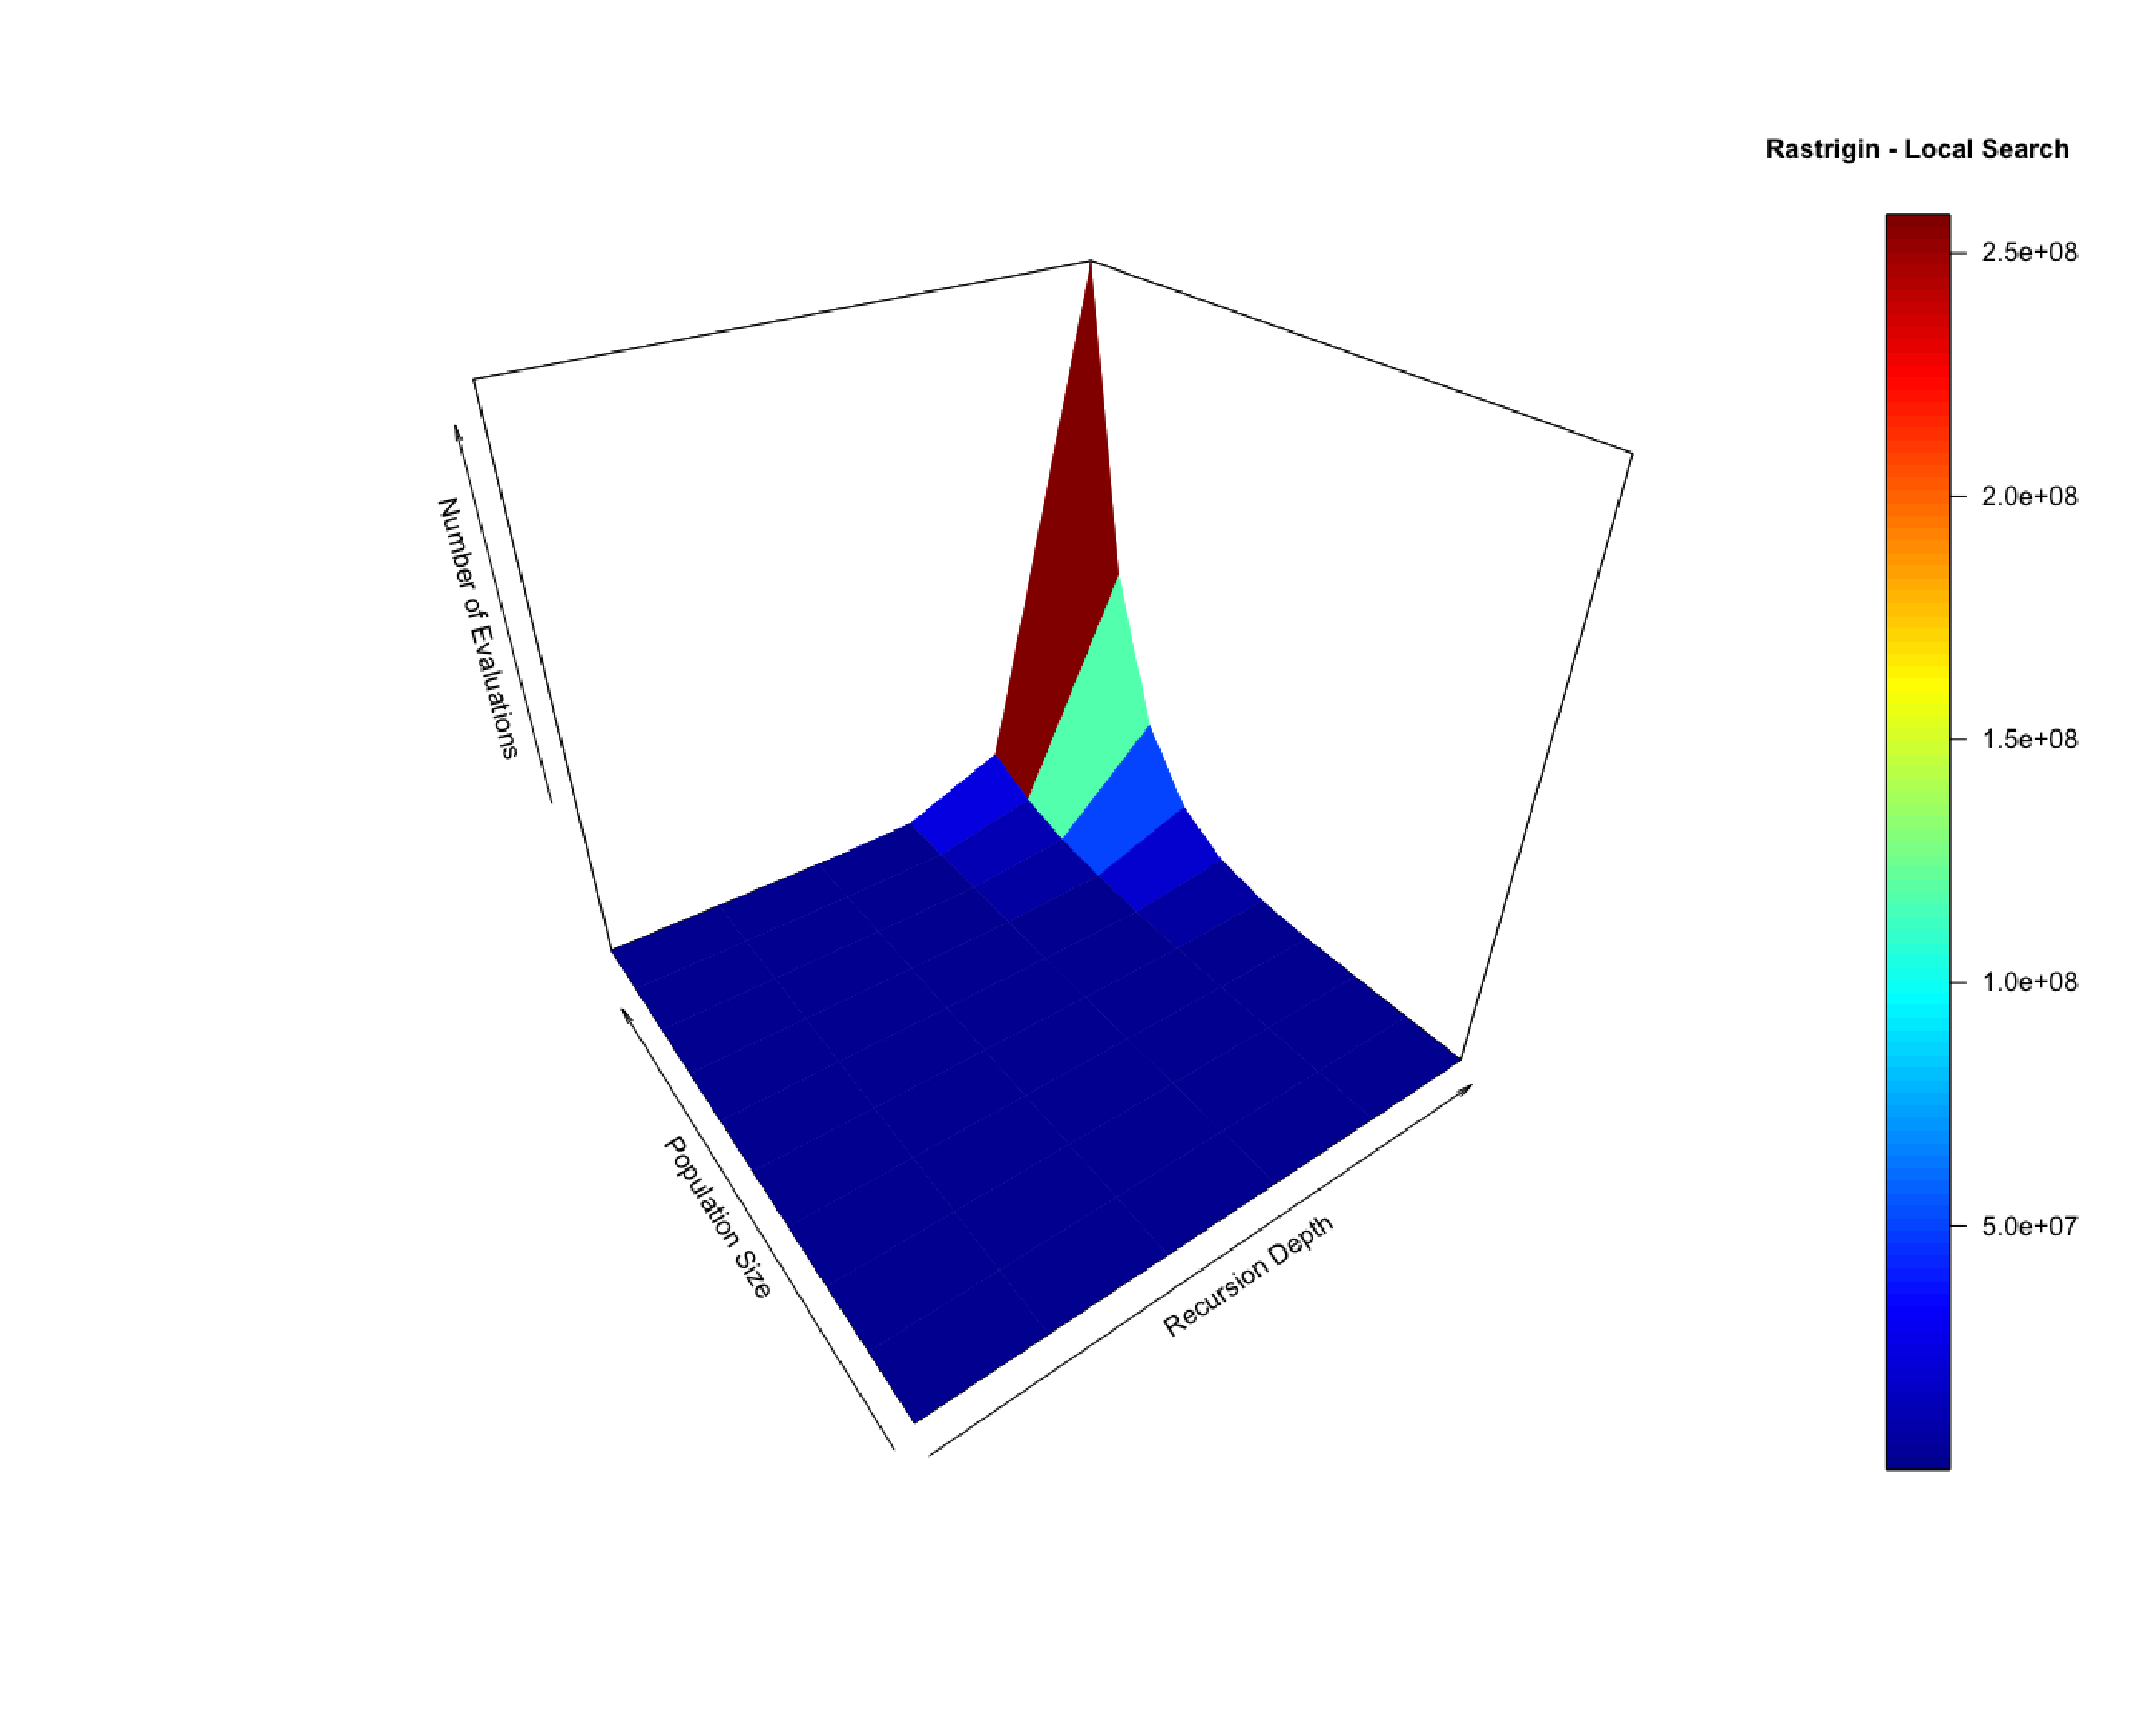
\includegraphics[width=1.0\hsize,height=0.65\hsize]{fig13.eps}
\caption{Rastrigin - Local Search - Fitness Evaluations}
\label{fig24}
\end{figure}

\begin{figure}[tbp]
\centering
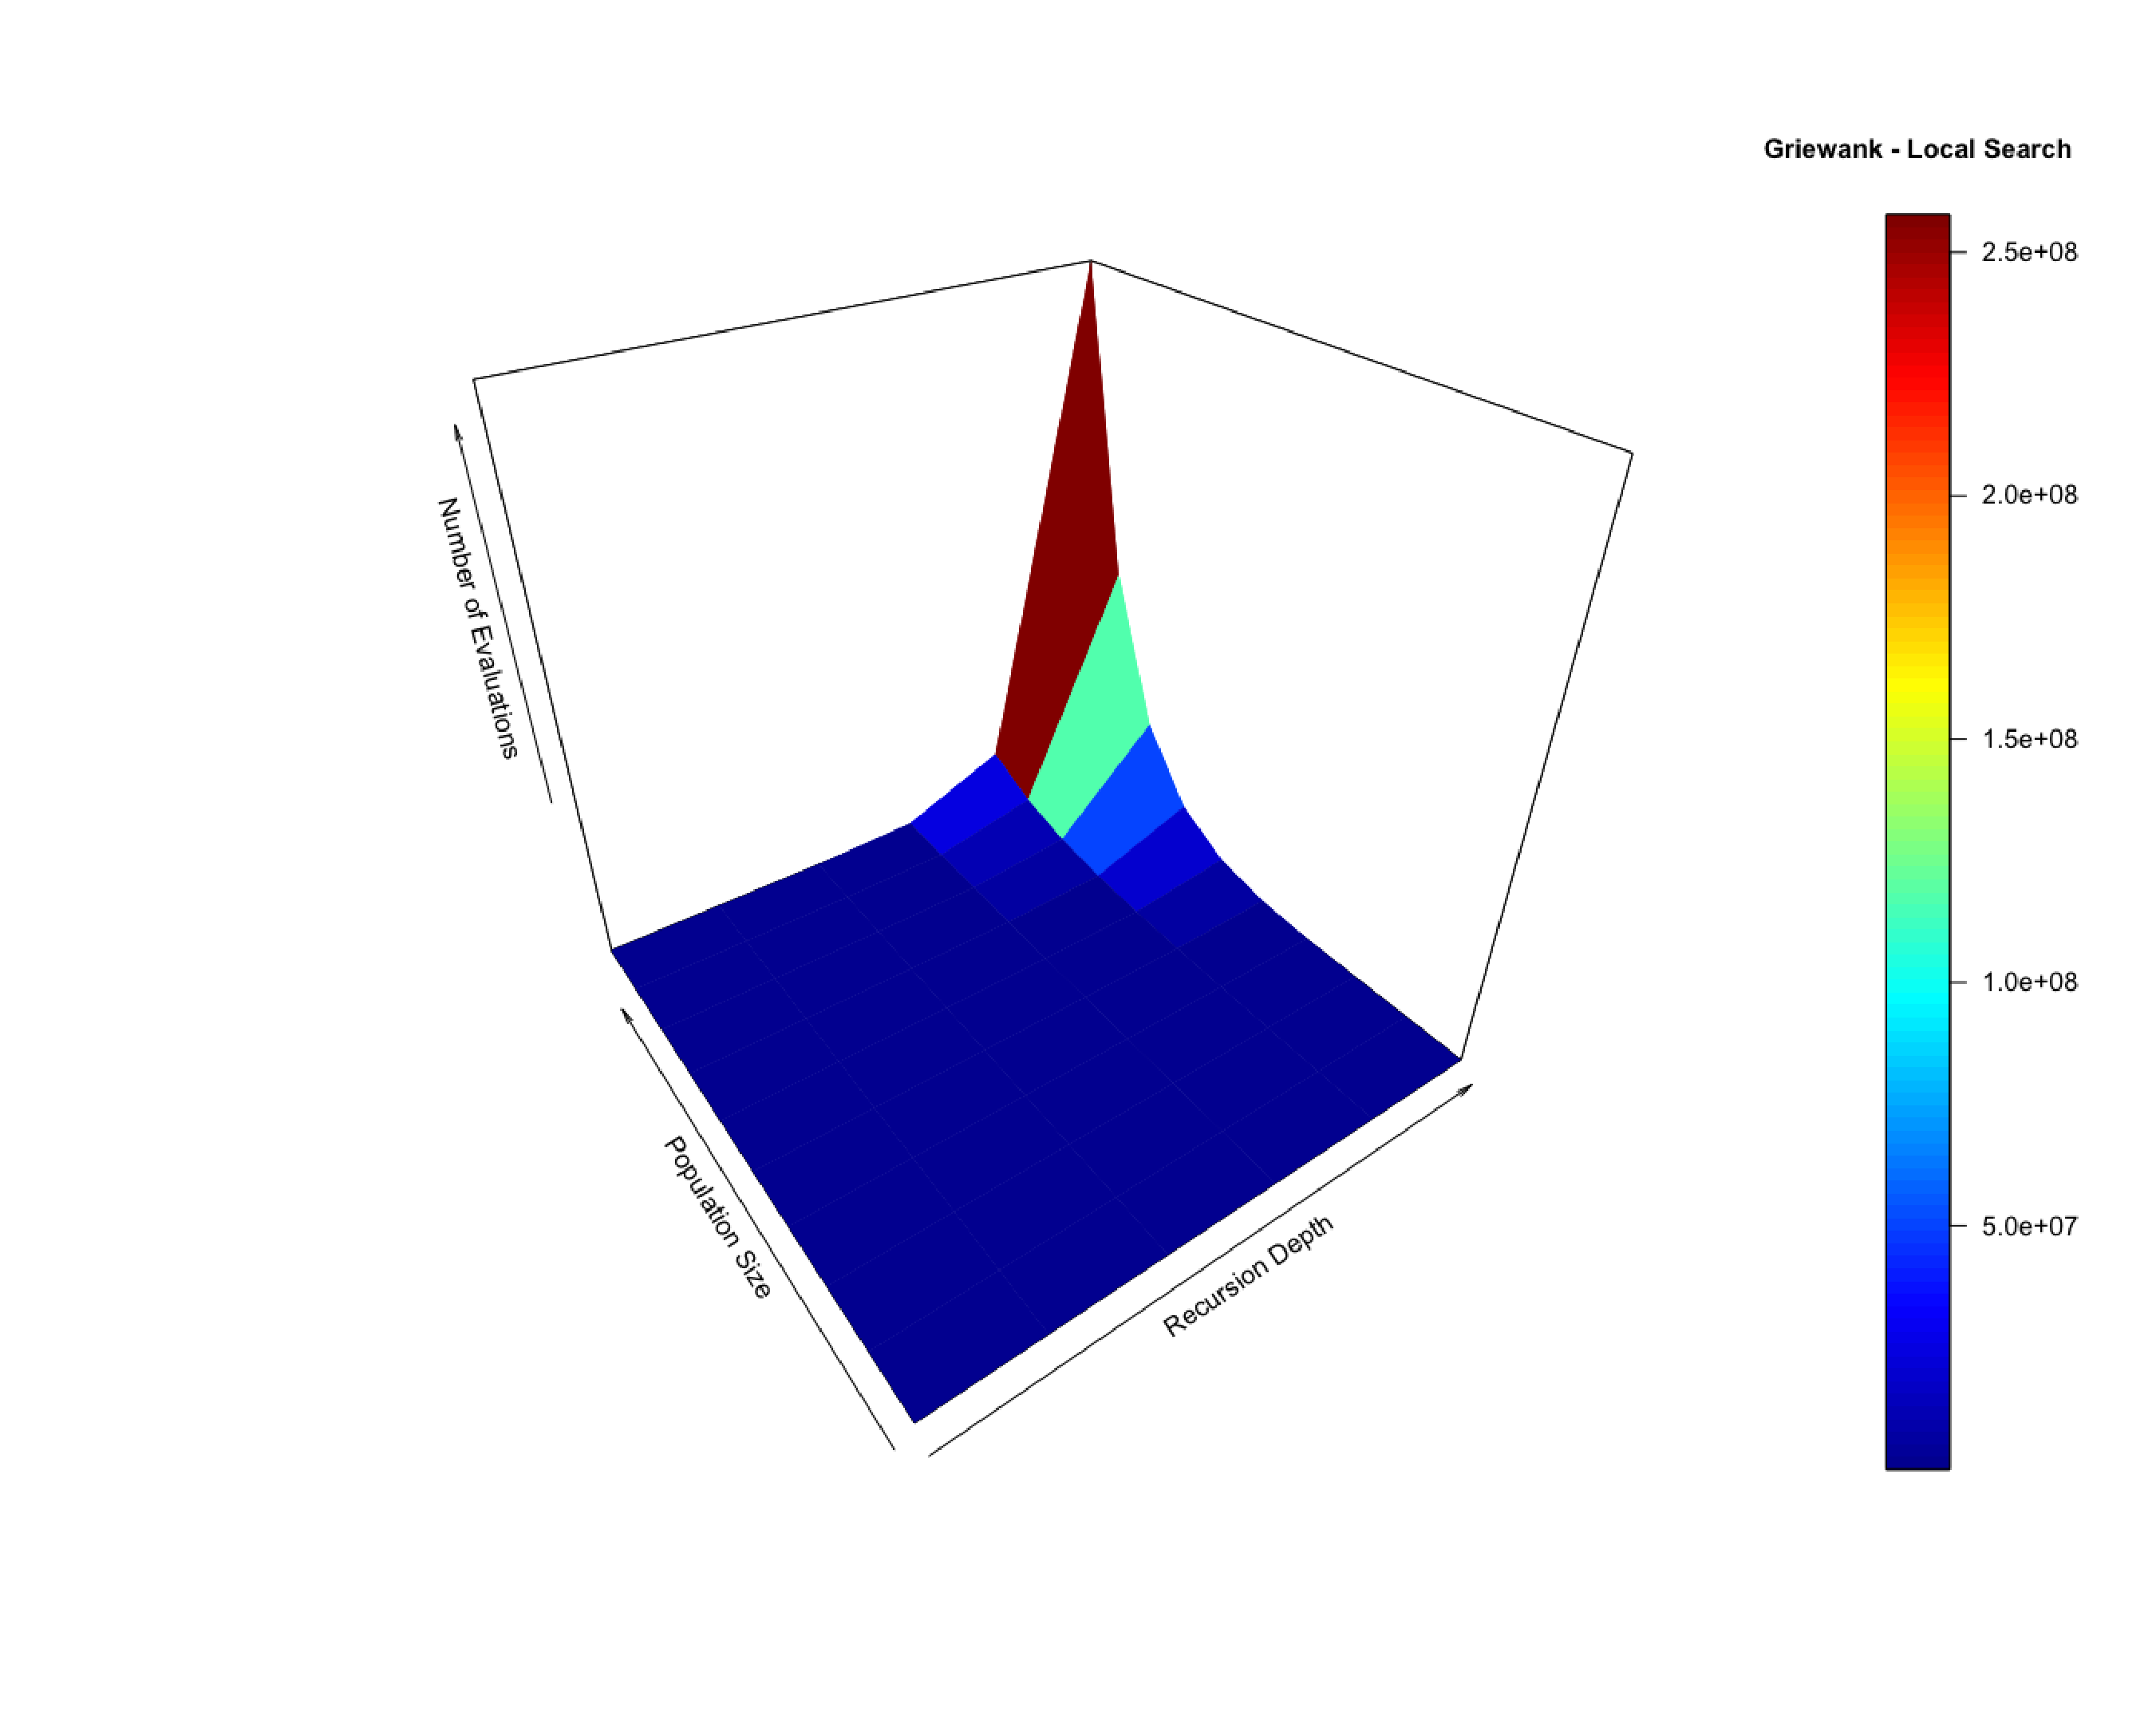
\includegraphics[width=1.0\hsize,height=0.65\hsize]{fig16.eps}
\caption{Griewank - Local Search - Fitness Evaluations}
\label{fig25}
\end{figure}

\begin{figure}[tbp]
\centering
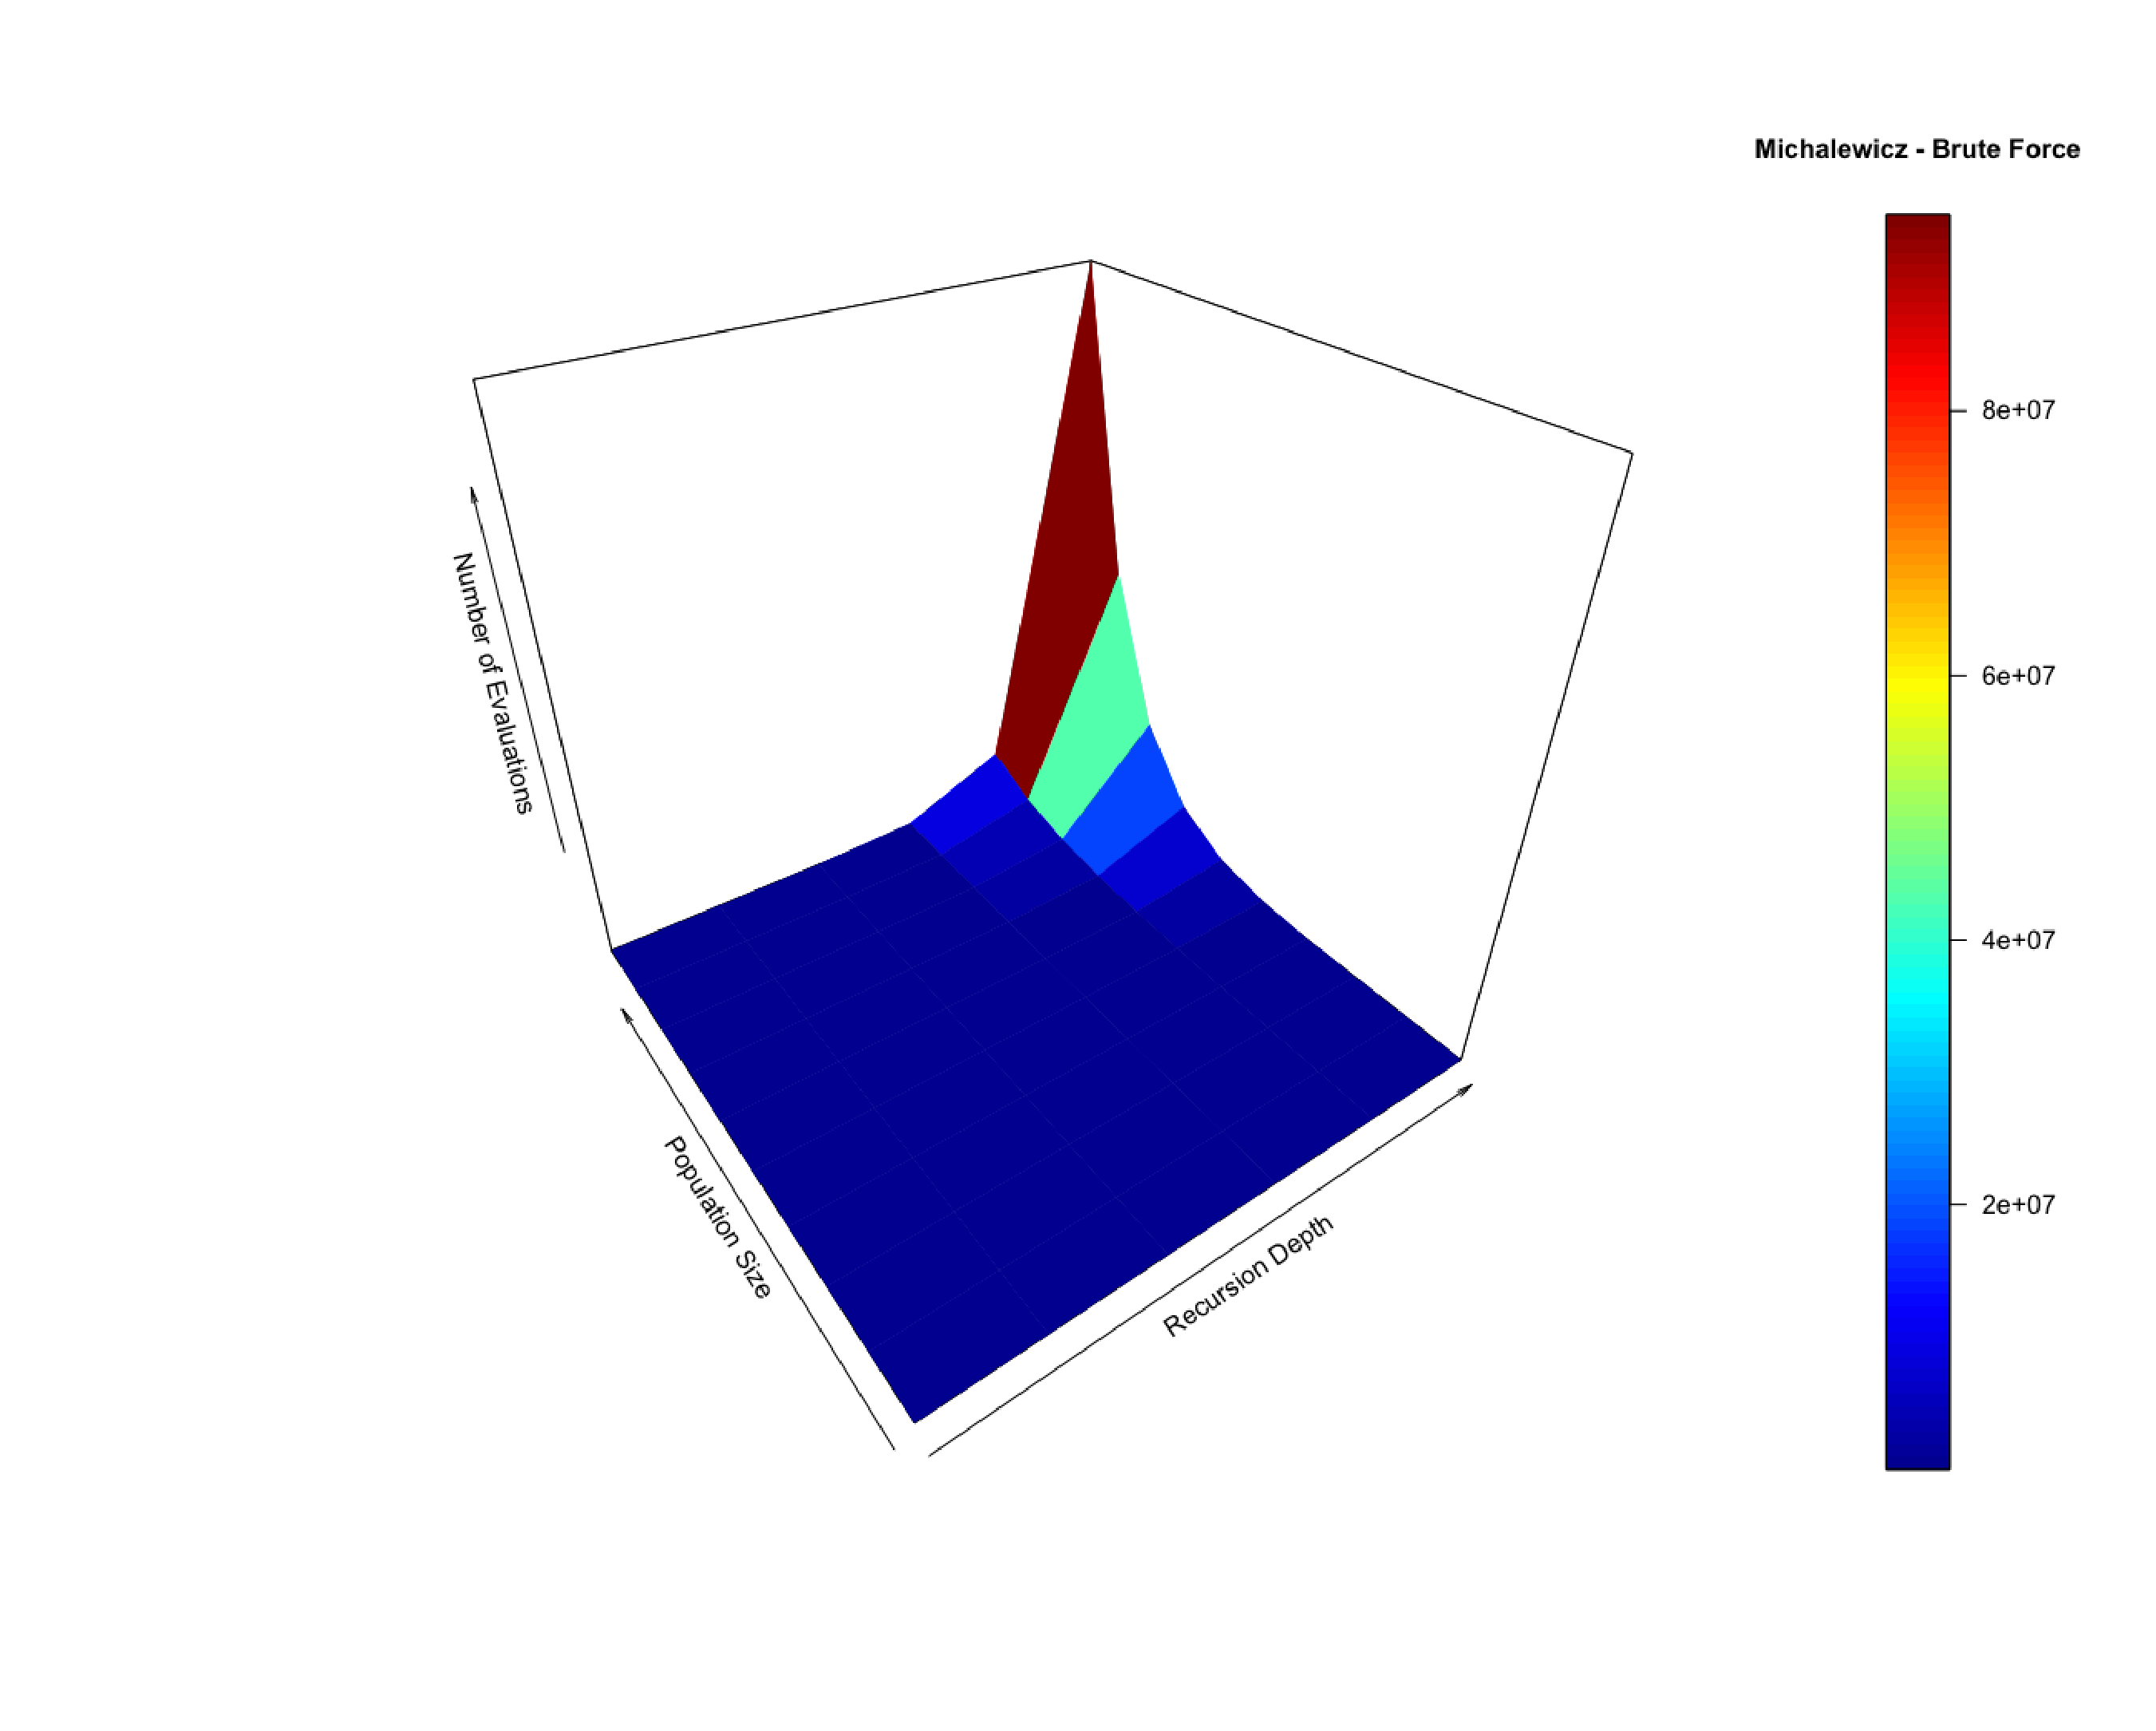
\includegraphics[width=1.0\hsize,height=0.65\hsize]{fig19.eps}
\caption{Michalewicz - Brute Force - Fitness Evaluations}
\label{fig26}
\end{figure}

\begin{figure}[tbp]
\centering
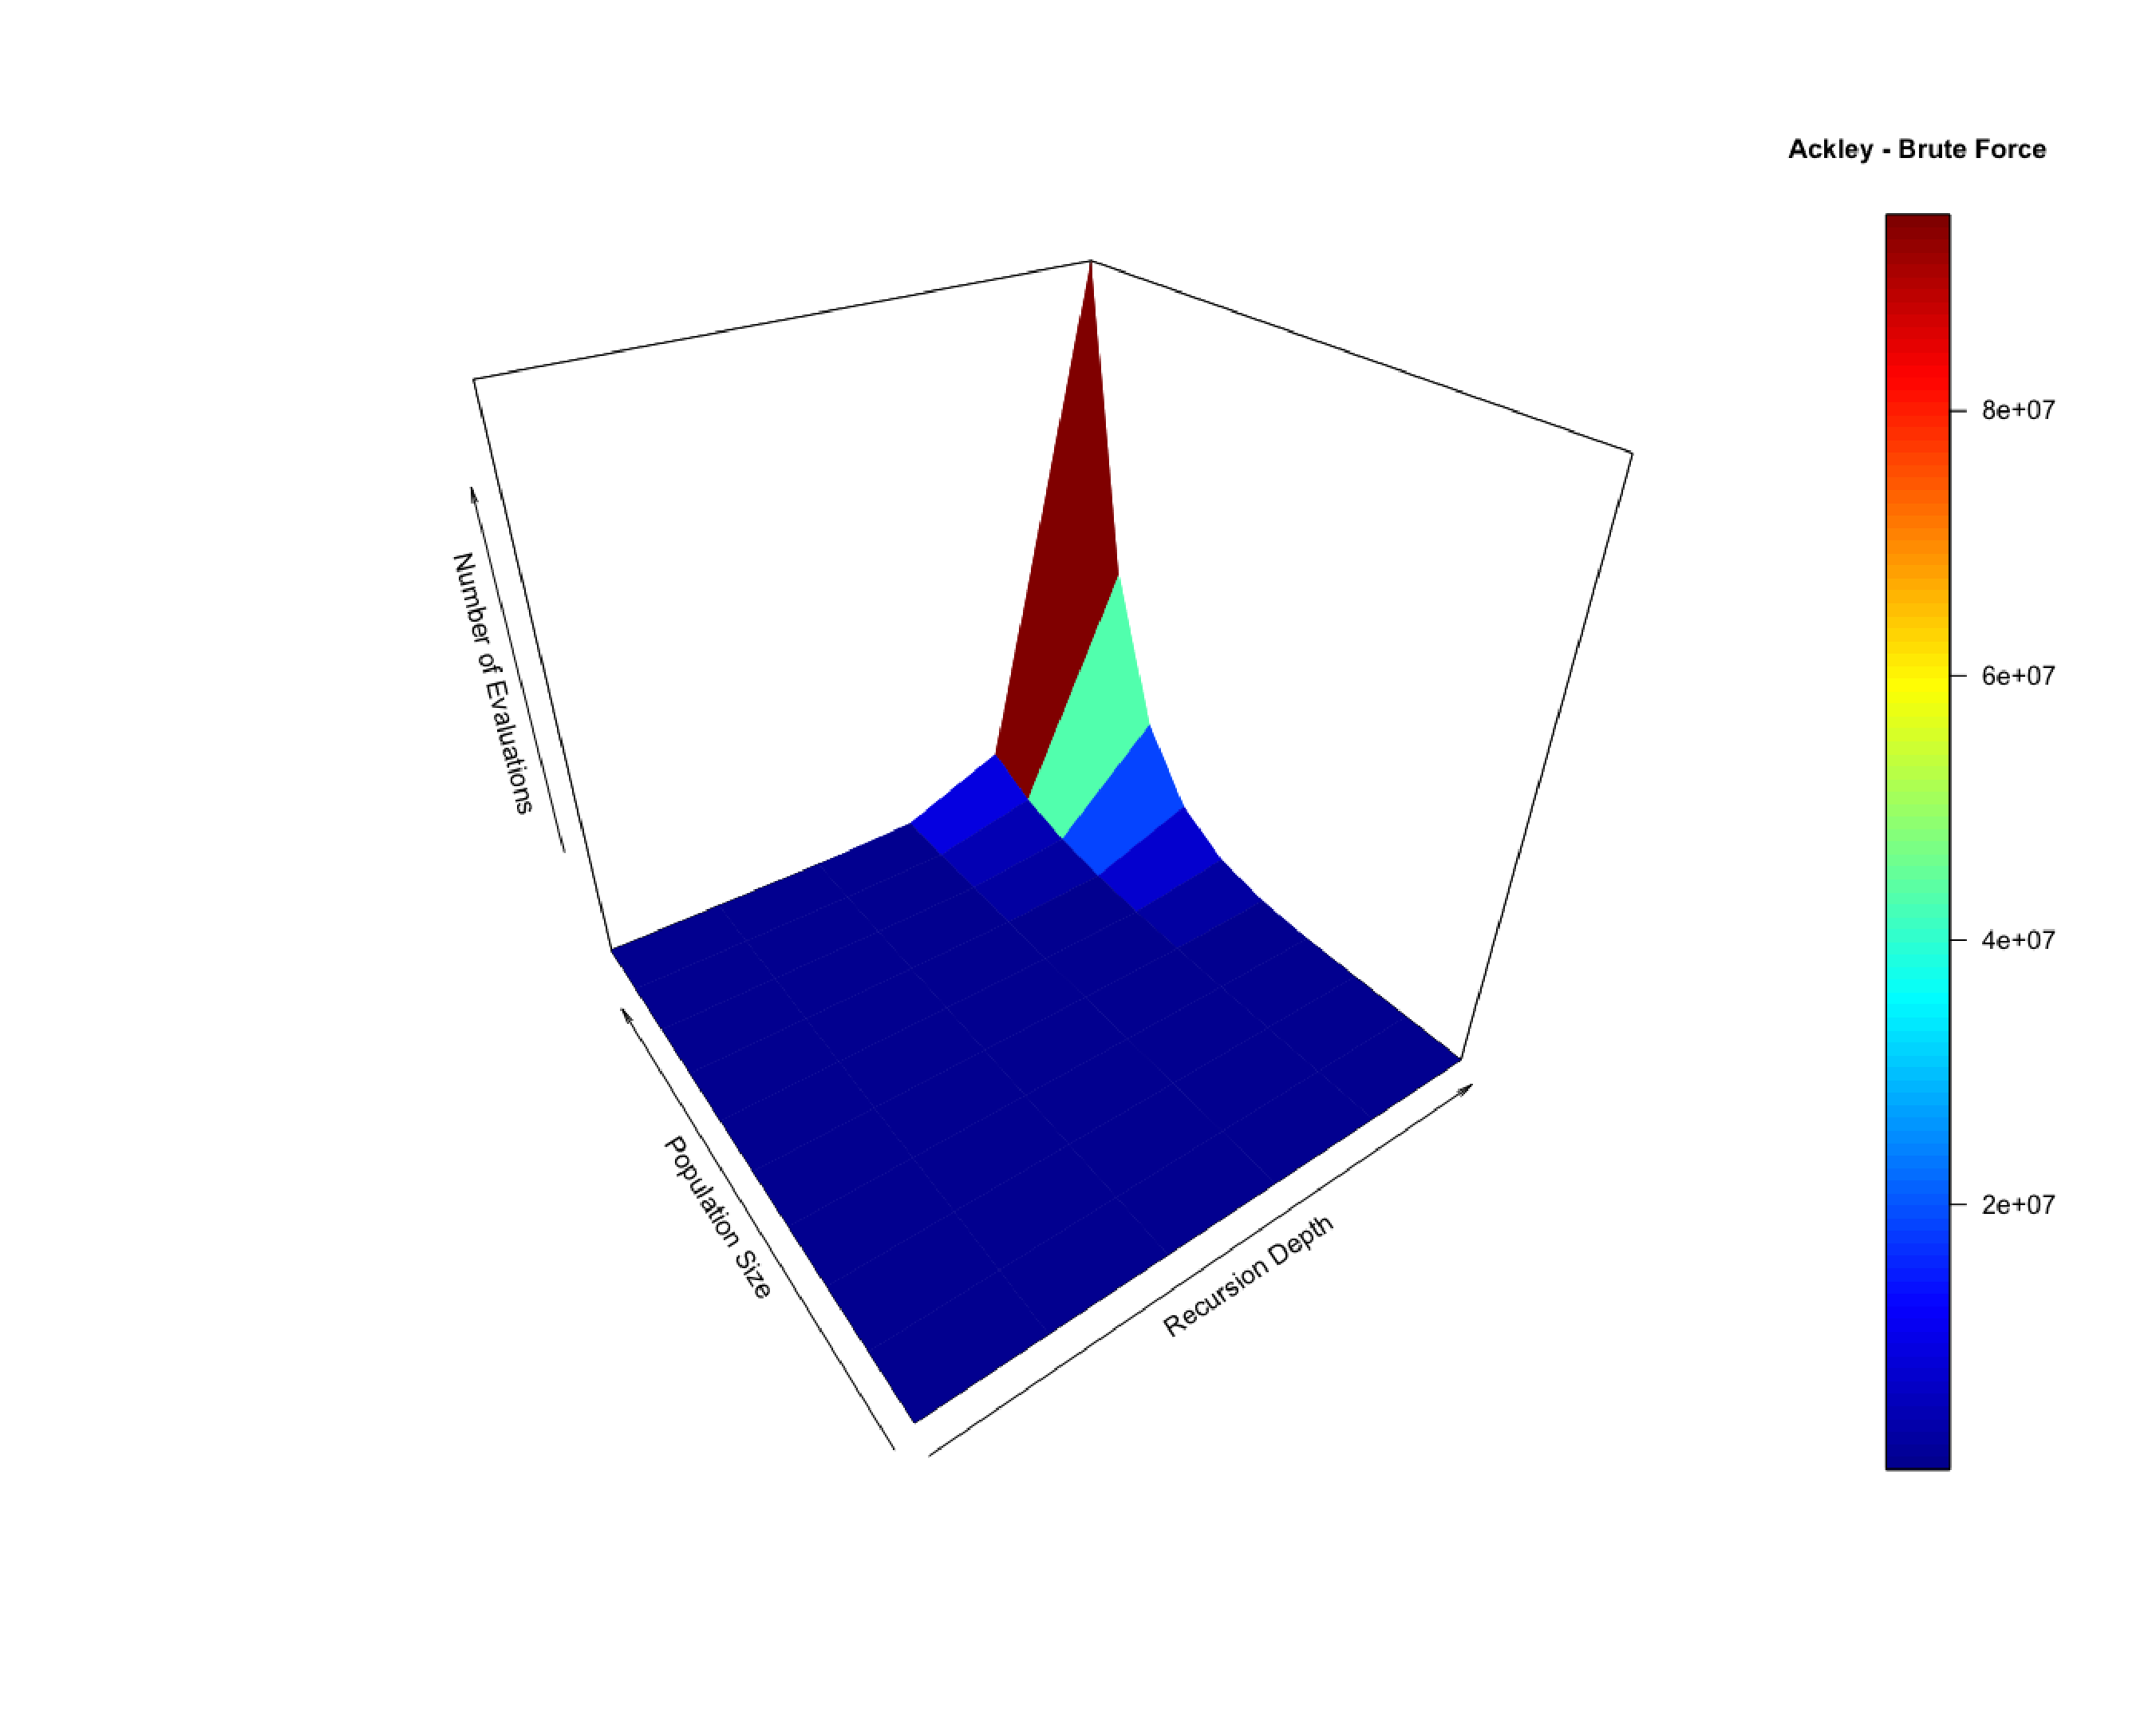
\includegraphics[width=1.0\hsize,height=0.65\hsize]{fig22.eps}
\caption{Ackley - Brute Force - Fitness Evaluations}
\label{fig27}
\end{figure}

\begin{figure}[tbp]
\centering
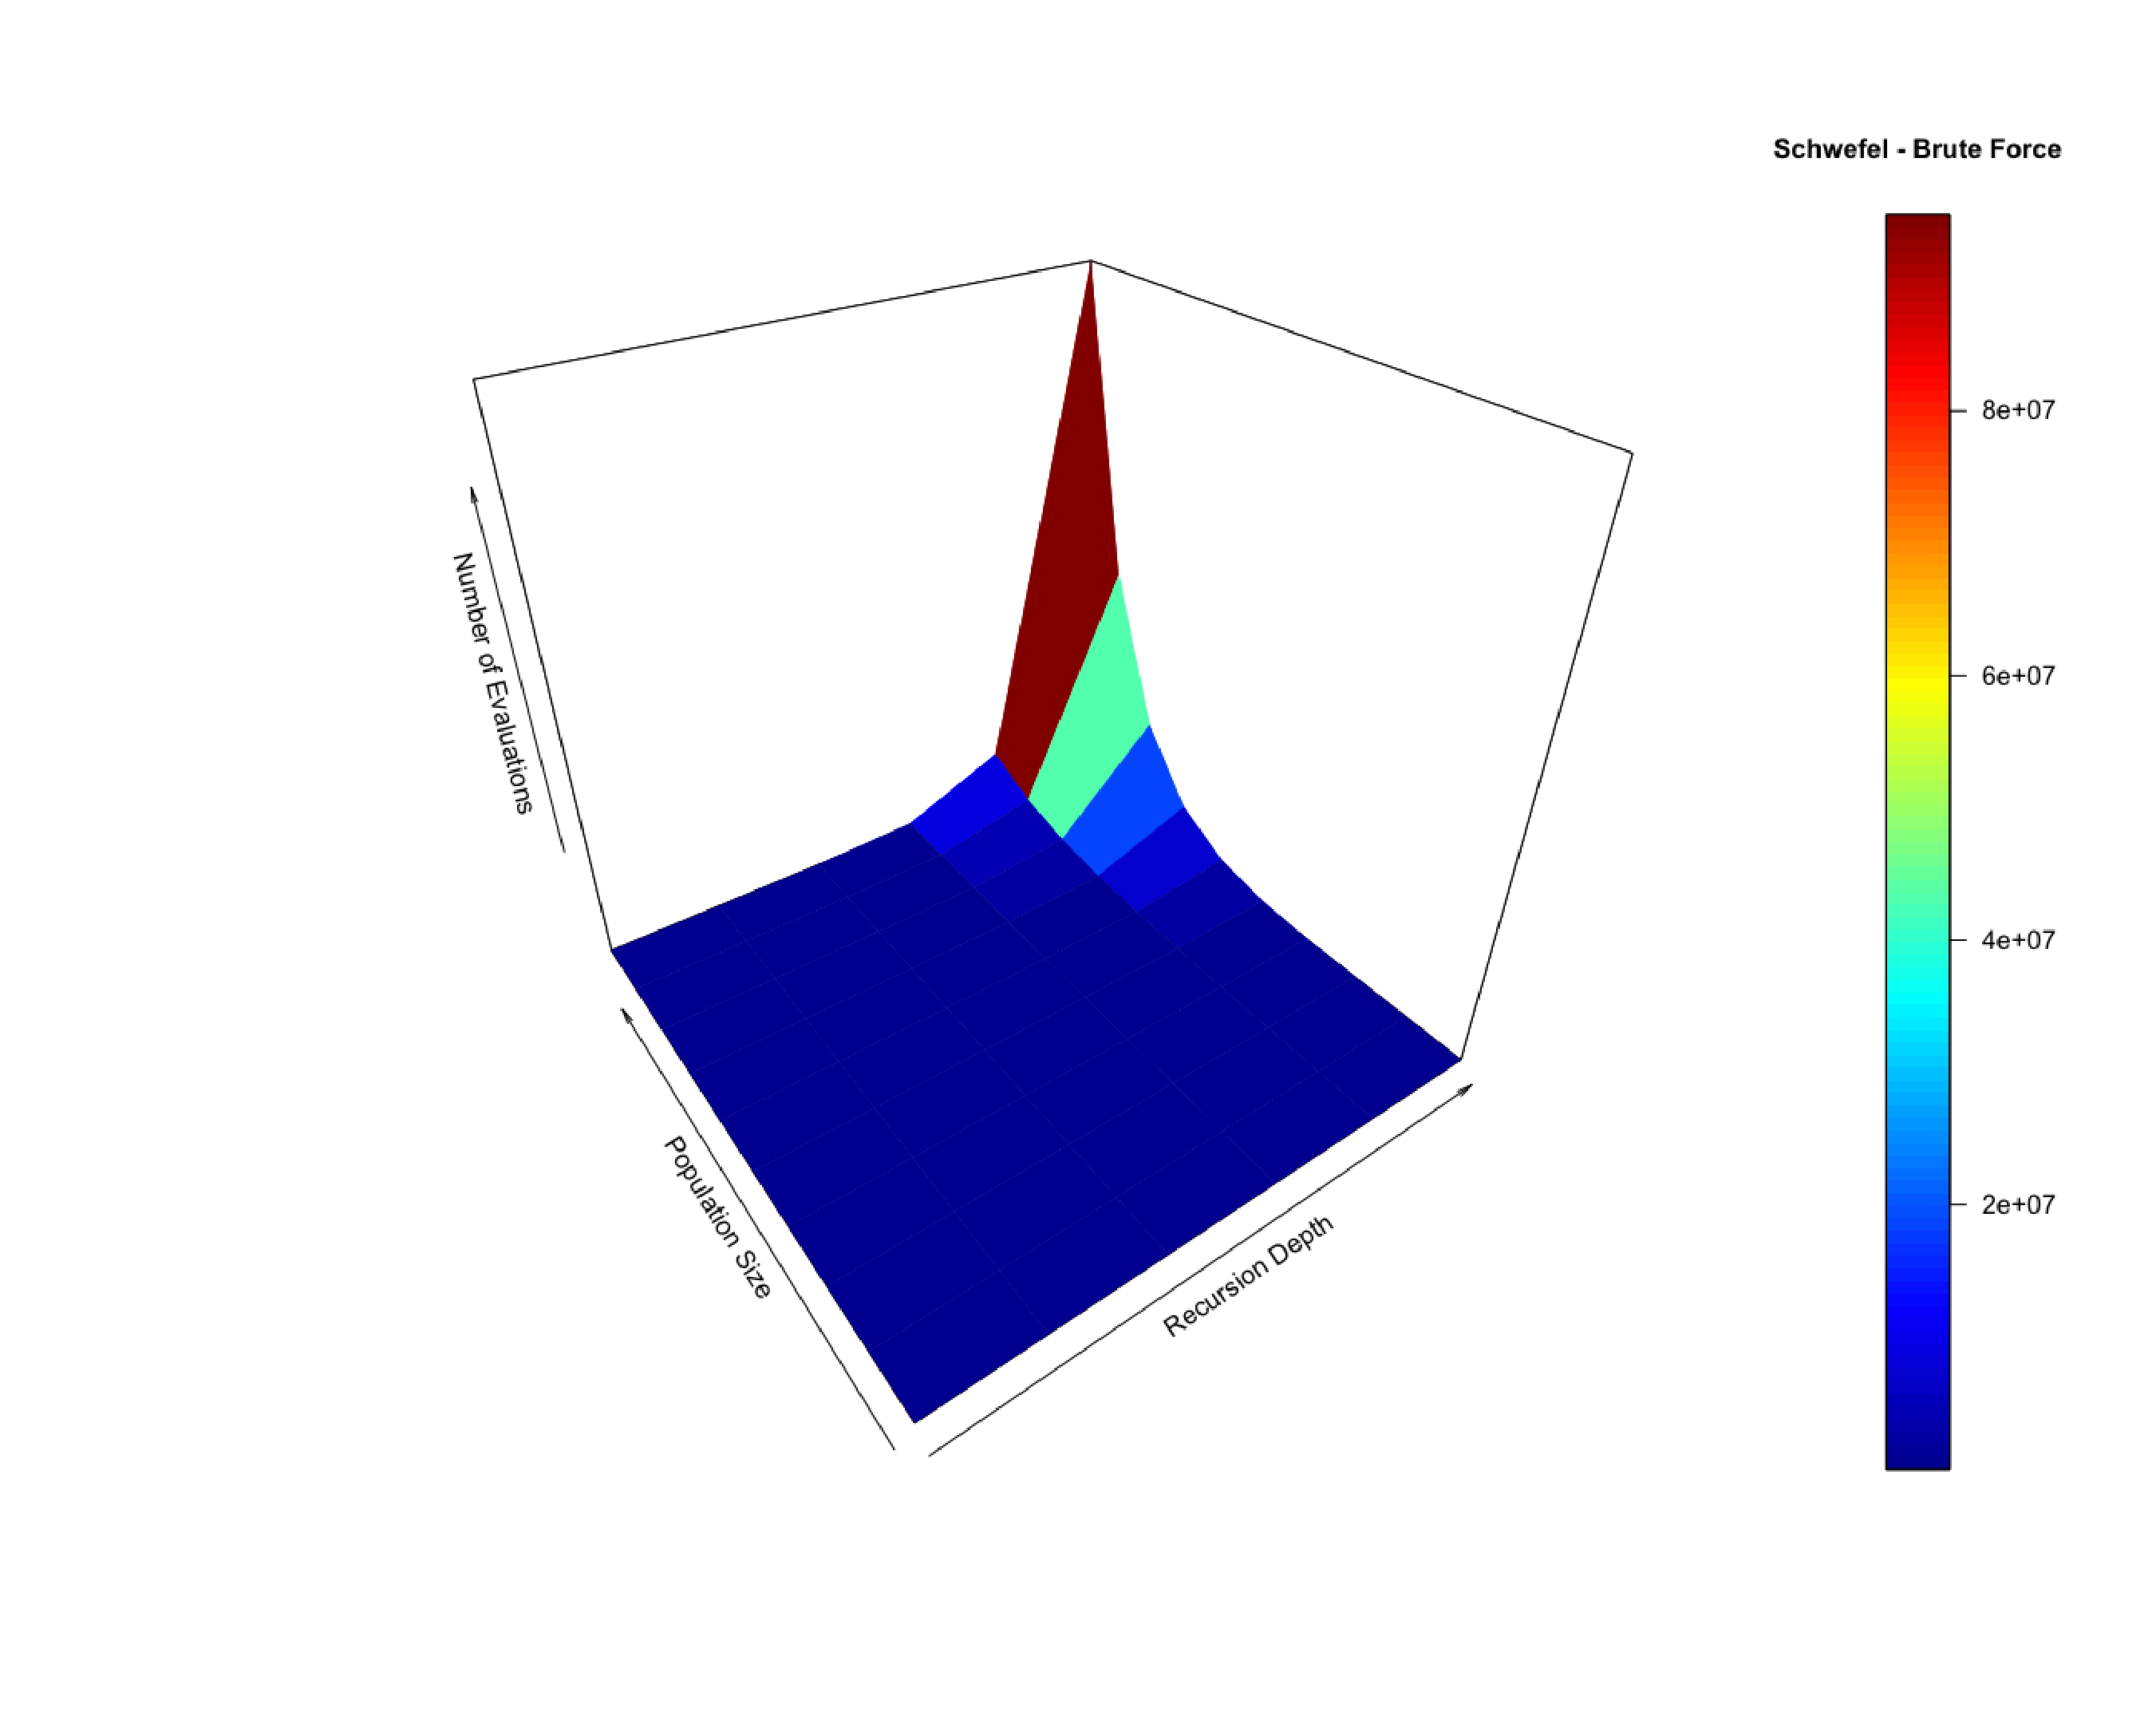
\includegraphics[width=1.0\hsize,height=0.65\hsize]{fig25.eps}
\caption{Schwefel - Brute Force - Fitness Evaluations}
\label{fig28}
\end{figure}

\begin{figure}[tbp]
\centering
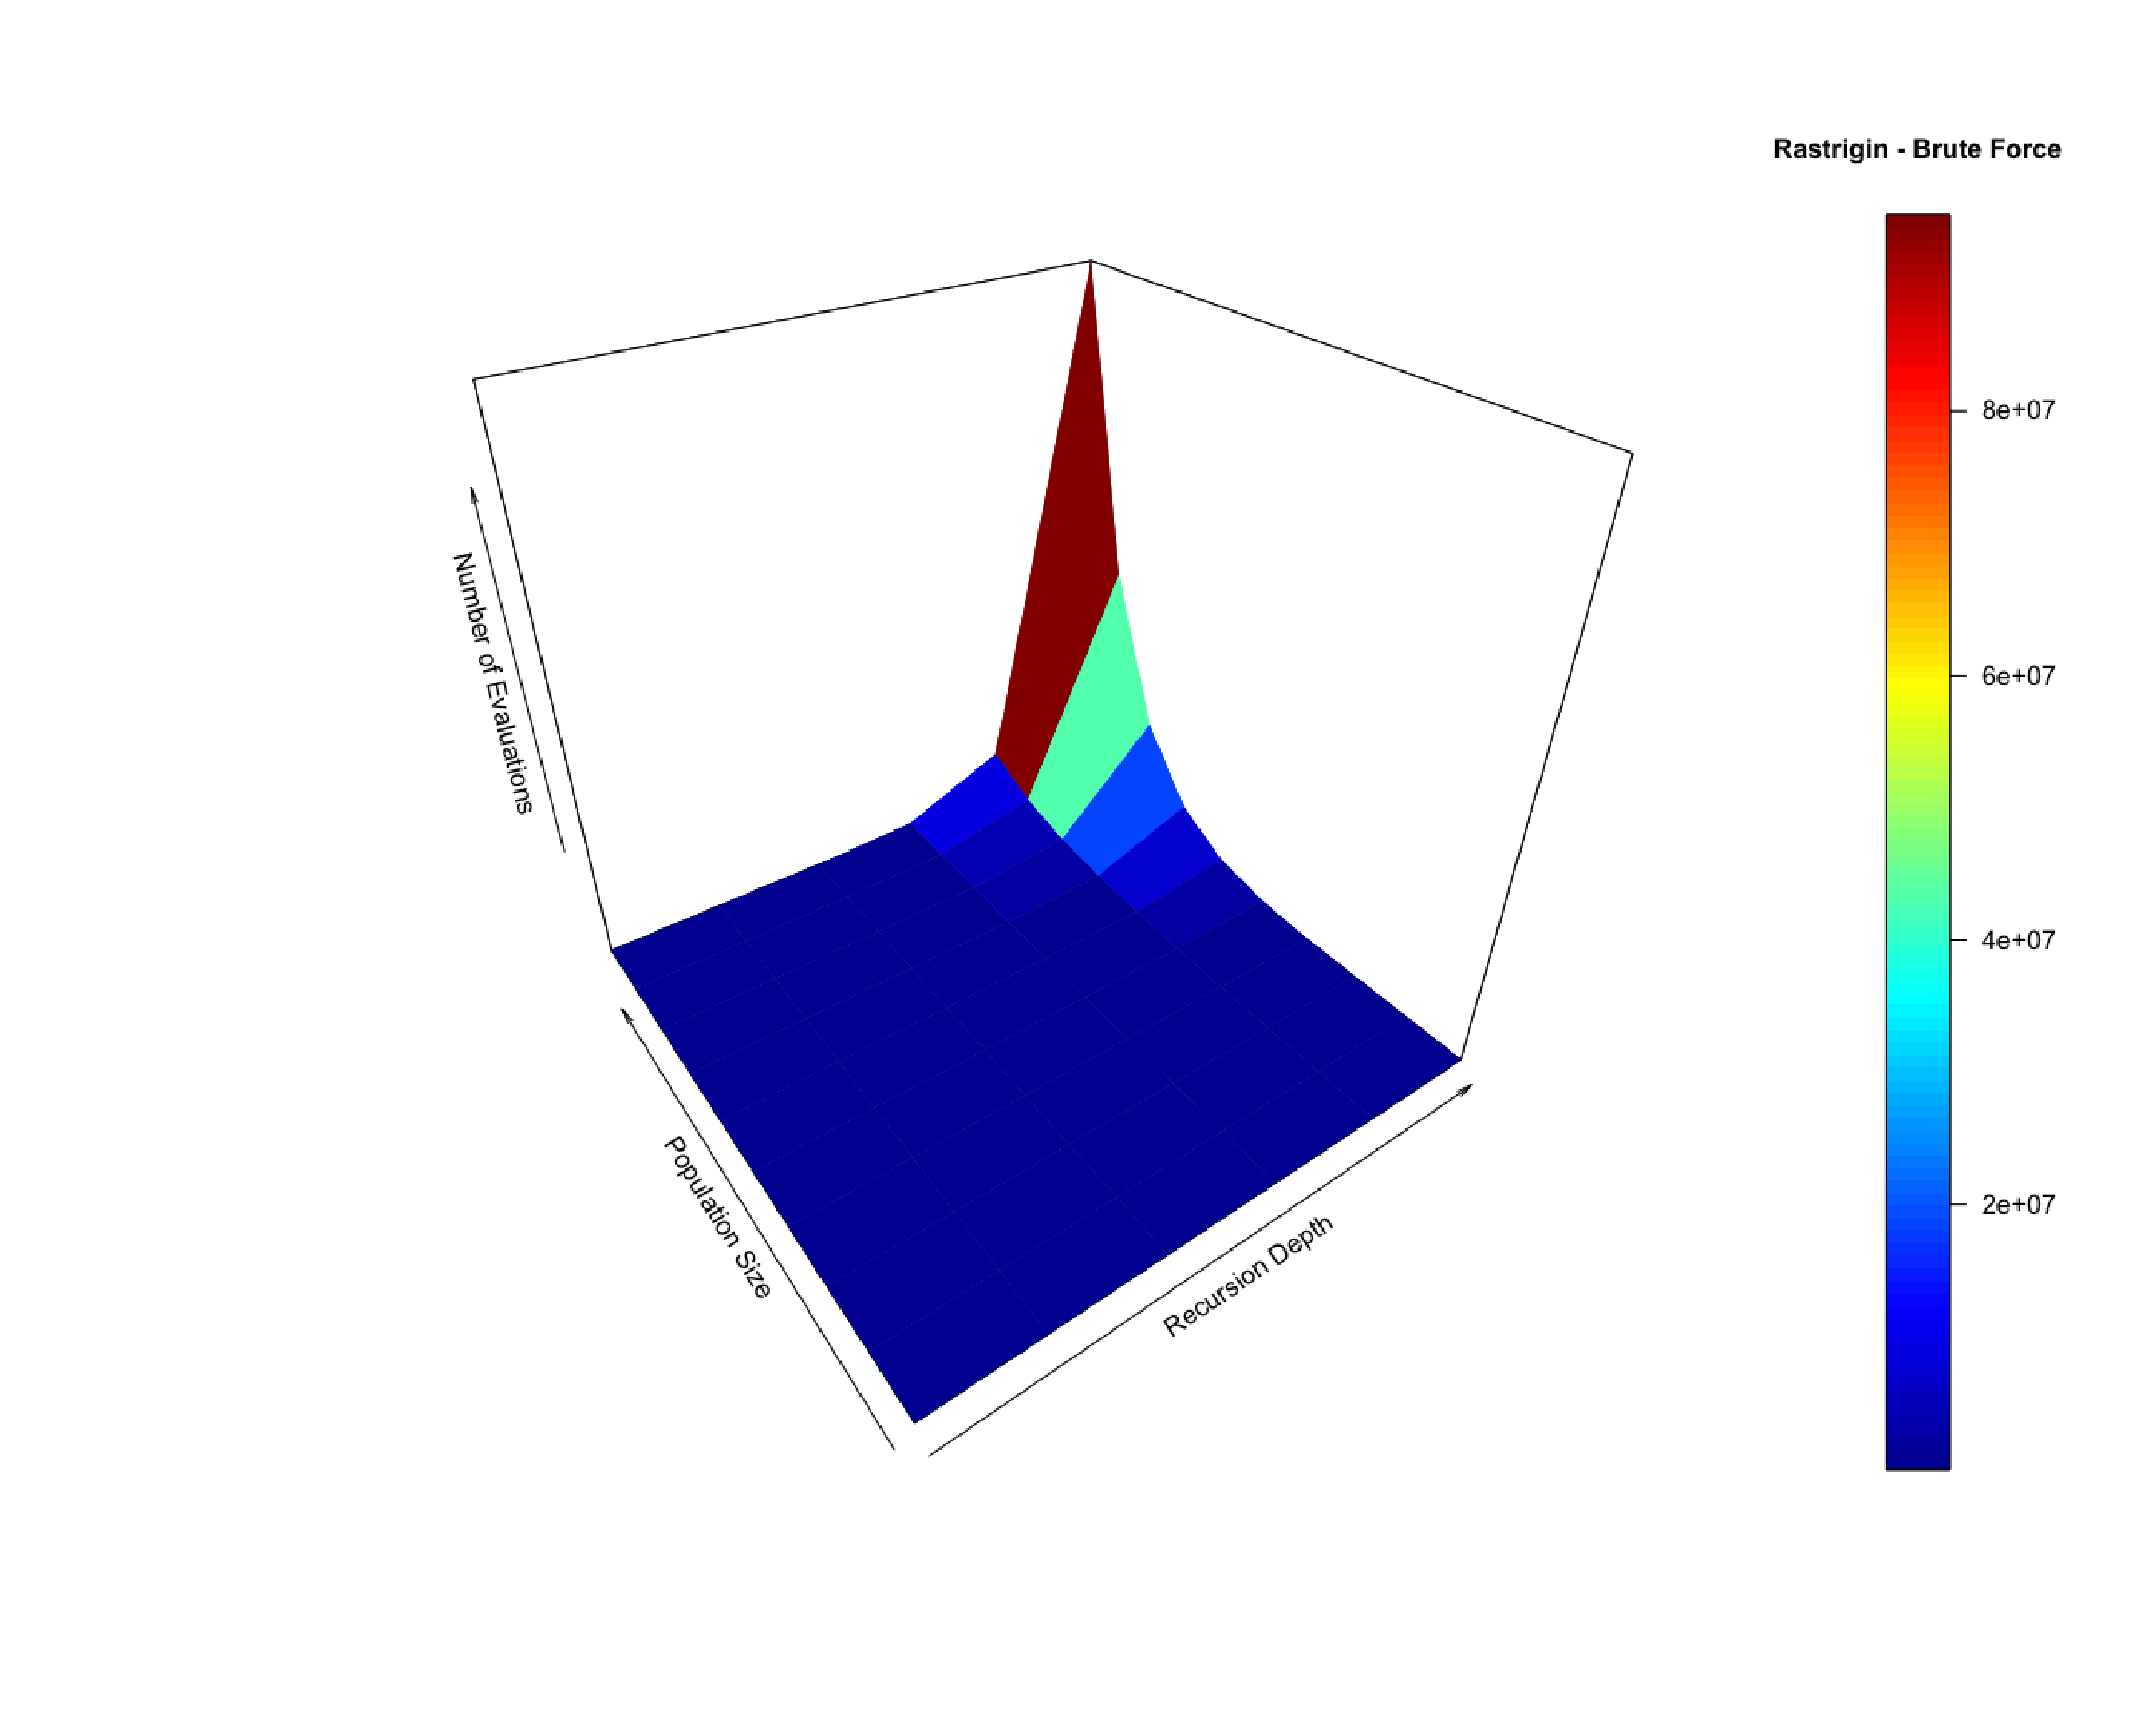
\includegraphics[width=1.0\hsize,height=0.65\hsize]{fig28.eps}
\caption{Rastrigin - Brute Force - Fitness Evaluations}
\label{fig29}
\end{figure}

\begin{figure}[tbp]
\centering
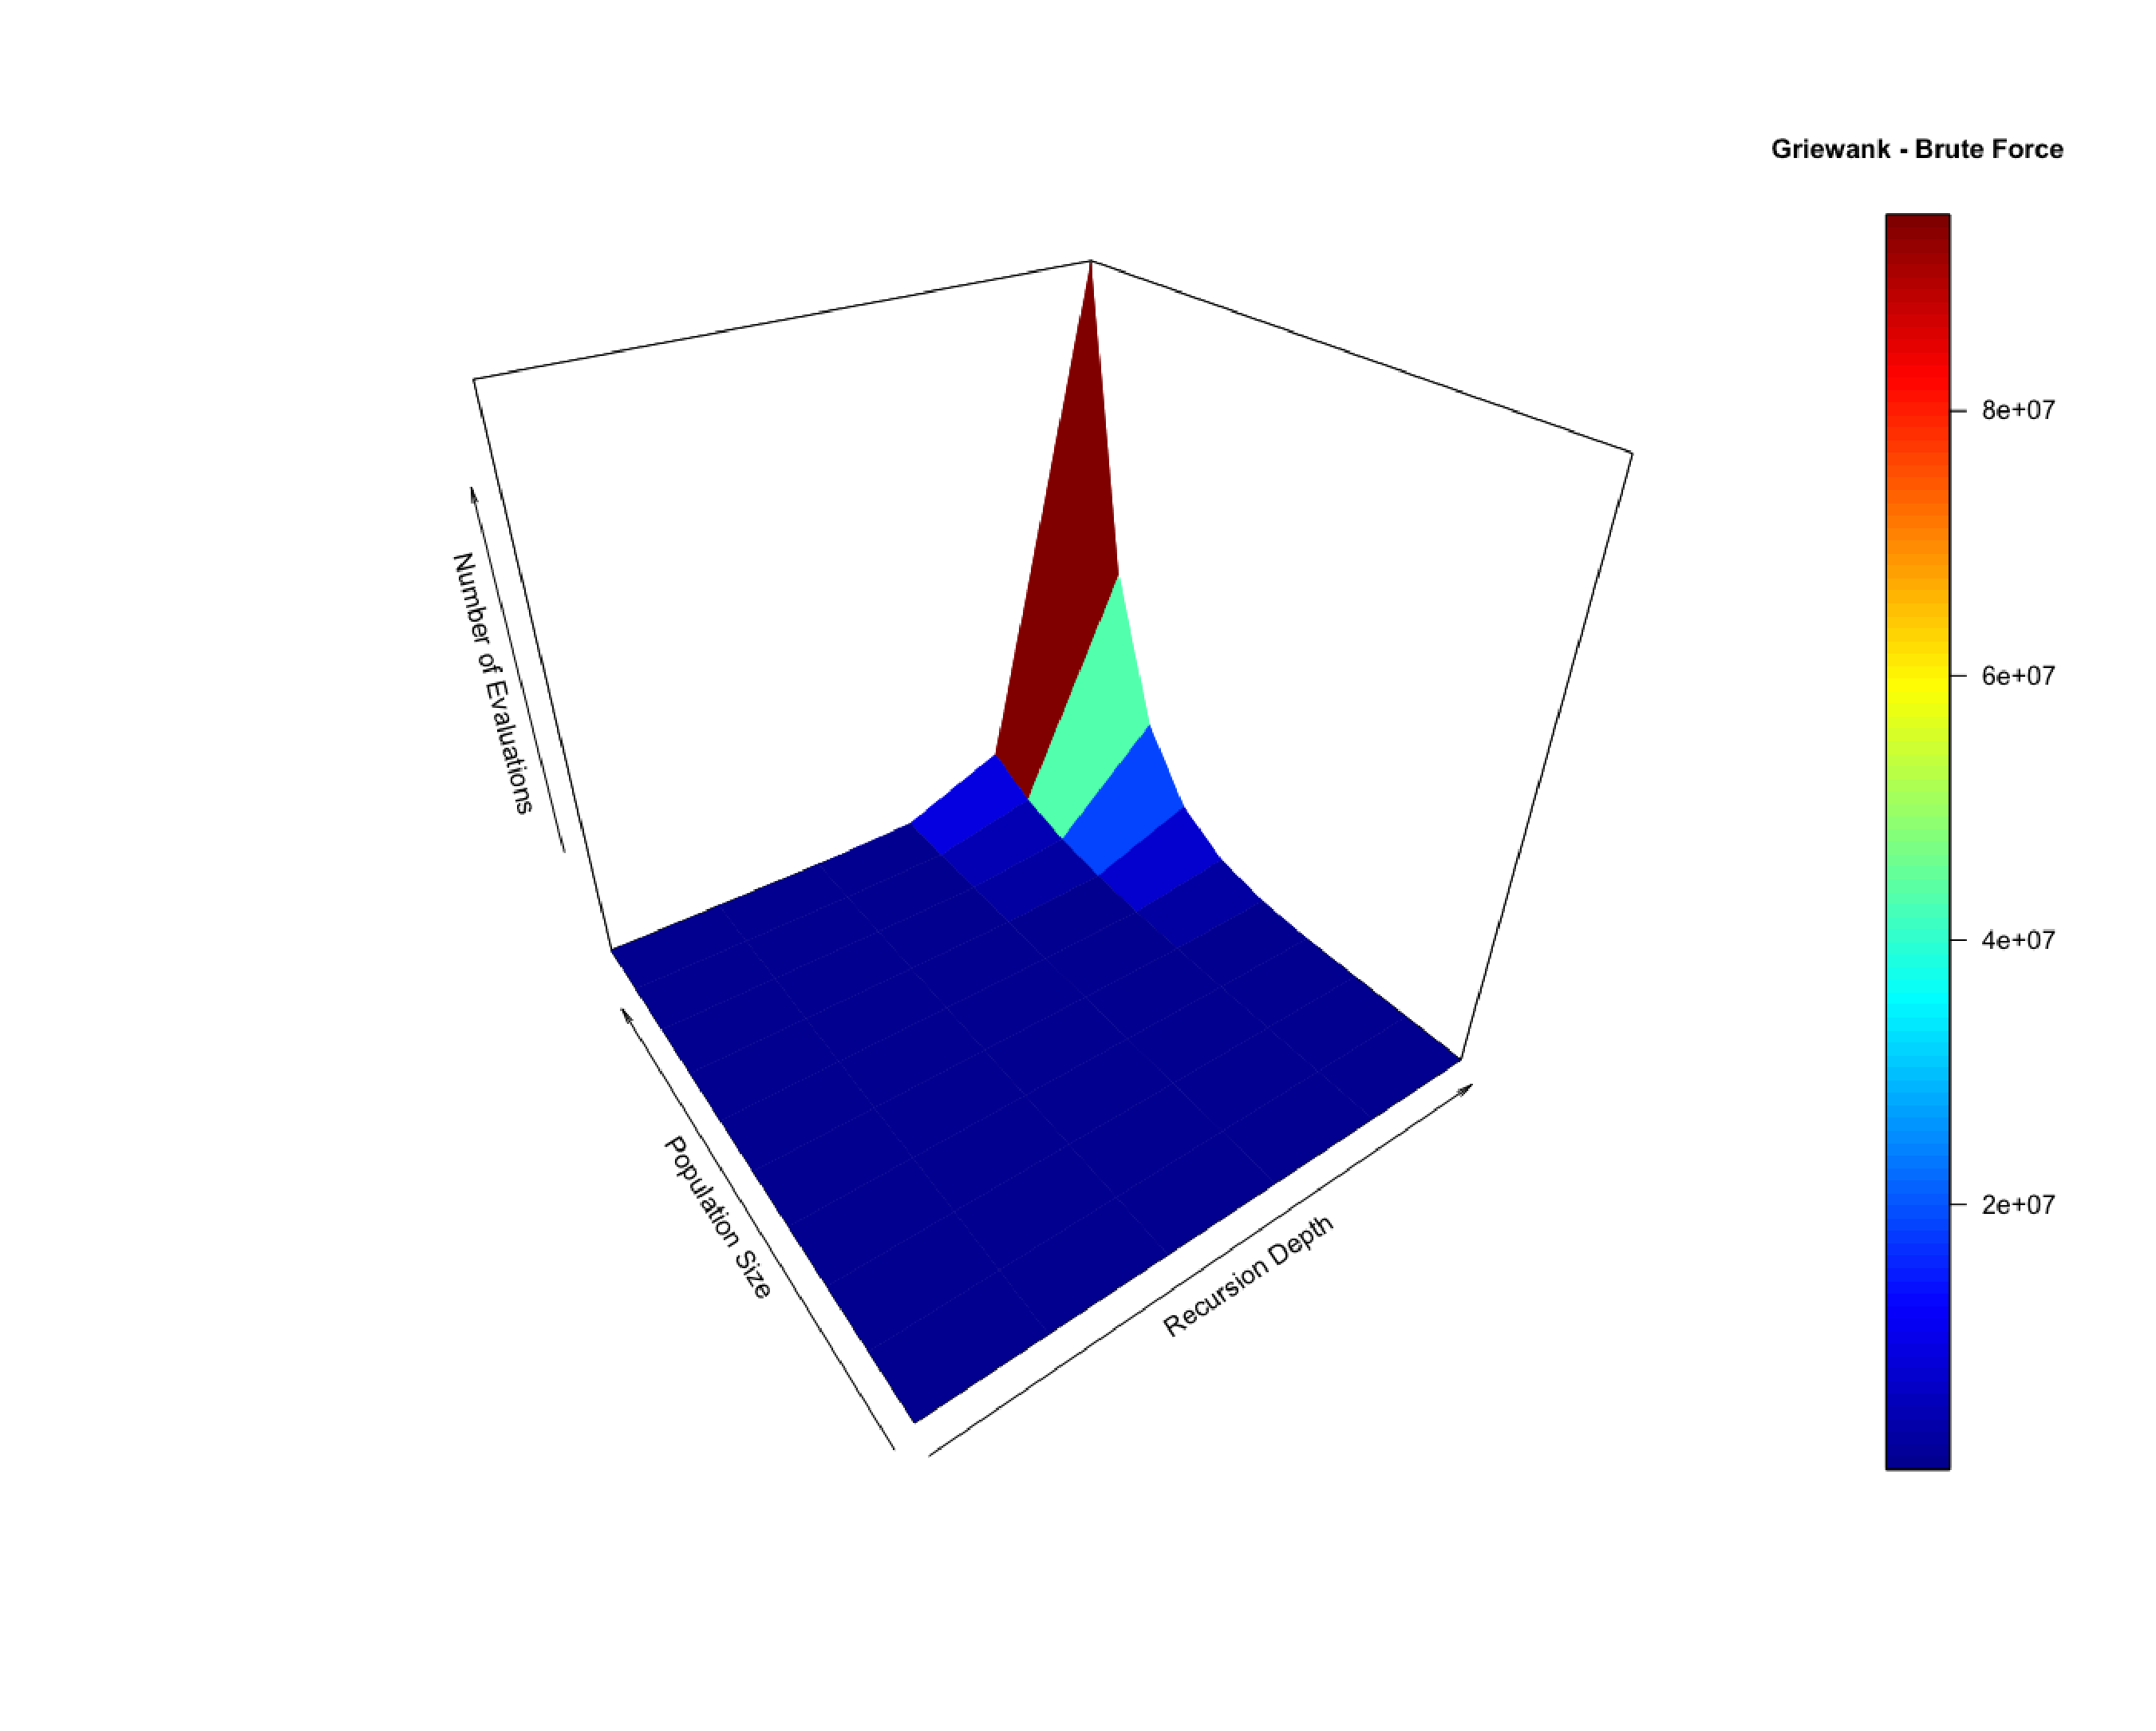
\includegraphics[width=1.0\hsize,height=0.65\hsize]{fig31.eps}
\caption{Griewank - Brute Force - Fitness Evaluations}
\label{fig30}
\end{figure}

\section{Conclusion}

This research extends the brute-force part of the recursive descent procedure in genetic algorithms selection operator with local search. The experimental results show very good efficiency but it comes with the price of higher computational time. Because of the higher computational time, the proposed selection can be used for tasks that have no strict time limitations. As further research, it will be interesting the same selection operator to be implemented in algorithms like differential evolution \cite{reddy-01} with different sizes of the sub-populations \cite{koumousis-01} on different recursive levels like small sizes on low levels and bigger sizes on higher levels. 

\section*{Acknowledgment}

This research is funded by Velbazhd Software LLC and it is partially supported by the Bulgarian Ministry of Education and Science (contract D01–205/23.11.2018) under the National Scientific Program ``Information and Communication Technologies for a Single Digital Market in Science, Education and Security (ICTinSES)'', approved by DCM \# 577/17.08.2018.

\begin{thebibliography}{99}

\bibitem{matsui-01} K. Matsui, ``New selection method to improve the population diversity in genetic algorithms,'' {\it in IEEE International Conference on Systems, Man, and Cybernetics,} Japan, 1999.

\bibitem{alander-01} J. Alander, ``On Optimal Population Size of Genetic Algorithms,'' {\it in Computer Systems and Software Engineering,} Netherlands, 1992.

\bibitem{fellows-01} M. Fellows, F. Fomin, D. Lokshtanov, F. Rosamond, S. Saurabh and Y. Villanger, ``Local Search Is Brute-Force Avoidable,'' {\it in Journal of Computer and System Sciences,} vol.~78, no.~3, 2012.

\bibitem{gelfand-01} S. Gelfand, and S. Mitter, ``Recursive Stochastic Algorithms for Global Optimization in $R^d$,'' {\it in SIAM Journal on Control and Optimization,} 1991.

\bibitem{wang-01} Q.Wang, ``The Genetic Algorithm and Its Application to Calibrating Conceptual Rainfall‐Runoff Models,'' {\it in Water Resoruces Research,} vol.~27, no.~9, 1991.

\bibitem{back-01} T. Back, ``Self-Adaptation in Genetic Algorithms,'' {\it in The First European Conference on Artificial Life,} 1992.

\bibitem{miller-01} B. Miller and D. Goldberg, ``Genetic Algorithms, Tournament Selection, and the Effects of Noise,'' {\it in Complex Systems,} vol.~9, 1995.

\bibitem{grefenstette-01} J. Grefenstette, ``Rank-based Selection,'' {\it in Evolutionary Computation,} 2000.

\bibitem{goldberg-01} D. Goldberg, ``A Note on Boltzmann Tournament Selection for Genetic Algorithms and Population-Oriented Simulated Annealing,'' {\it in Complex Systems,} vol.~4, 1990.

\bibitem{tomov-01} P. Tomov, I. Zankinski and T. Balabanov, ``Genetic Algorithm Selection Operator Based on Recursion and Brute-Force,'' {\it in 14th Annual Meeting of the Bulgarian Section of SIAM,} Fastumprint, 2019, pp.~93.

\bibitem{reddy-01} S. Surender Reddy and P. R. Bijwe, ``Differential evolution-based efficient multi-objective optimal power flow,'' {\it in Neural Computing and Applications,} vol.~31, 2019, pp.~509--522.

\bibitem{koumousis-01} V.K. Koumousis and C.P. Katsaras, ``A saw-tooth genetic algorithm combining the effects of variable population size and reinitialization to enhance performance,'' {\it in IEEE Transactions on Evolutionary Computation,} vol.~10, no.~1, 2006, pp.~19--28.

\end{thebibliography}

\end{document}
